%# -*- coding: utf-8-unix -*-
% !TEX program = xelatex
% !TEX root = ../thesis.tex
% !TEX encoding = UTF-8 Unicode
%%==================================================
%% chapter01.tex for SJTU Master Thesis
%%第五章
%%==================================================
\chapter{基于深度强化学习的飞机对抗策略}
\section{引言}
在上一章主要以双人棋盘类博弈策略进行描述,在本章将讨论非棋盘类单智能体对抗和二对二智能体对抗的问题。对于对称类棋盘游戏来说,其规则简单,并且可落子范围随着双方不断落子逐渐缩小,动作双方最多走满全盘步数即可或胜负,应用场景比较单一,对于其他应用场景还有待扩展,除此之外,现有的强化学习模型大多数针对单智能体游戏类的决策任务,对于两个以上智能体既有竞争又有合作的情况更加复杂,当对多智能体进行建模时,每一个智能体不仅需要感知外界环境,同时也需要及时获得其他智能体的信息,对于多智能体其动作空间和环境状态空间增大带来训练的困难。根据智能体之间的关系可以分为合作,竞争和既有竞争又有合作,对于这种比较复杂的模型,奖励的分配也是面临的难题之一。本章将介绍多智能体强化学习相关的理论算法基础后,设计一对一智能体相互对抗的实验场景,根据实际情况建立合理的状态动作以及奖励函数,并把实验场景拓展到二对二上,接着展示实验结果并进行分析。
\section{多智能体强化学习理论基础}
在多智能体研究中,智能体之间的关系可以是合作的、竞争的,也可以是两者兼而有之,许多算法都是为智能体特定的关系设立的。
如\cite{Lazaridou2017Multi}主要针对多智能体合作问题提出的,基于假设所有智能体的行为都是在提高集体奖励的基础上进行的。另一种方式是通过共享参数达到合作的目的\cite{Gupta2017Cooperative},这需要所有的智能体模型都相同,奖励也相同。这些算法一般不适用于竞争环境或混合环境。本章将就单智能体间的相互对抗拓展到多智能体间的组队形式的对抗,同队之间智能体是相互协作的,异队间智能体是相互对抗的,所有智能体的优化目标都是降低敌方奖励,增加本方奖励。
下面介绍常用的多智能体强化学习算法。
\subsection{Minimax-Q学习}
Minimax-Q\cite{Littman1994Markov}是一种适用于双人零和博弈的算法。其主要思想是两个智能体之间的奖励函数是互为相反数的,一方利益的最小化同时是另一方利益的最大化,所以两个智能体之间可以共享一个相同的奖励函数,是基于Q-learning算法进行实现的,Minimax-Q学习的值函数是Q值矩阵的最小最大化:
\begin{equation}
{{\rm{V}}^1}{\rm{(s) = }}\mathop {\max }\limits_{{\pi ^1} \in PD({A^1})} \mathop {\min }\limits_{{a^2} \in {A^2}} \sum\limits_{{a^1} \in {A^1}} {{Q_t}^1(s,{a^1},{a^2})} {\pi ^1}
\end{equation}
其中,${\pi ^1}$为第一个智能体的策略,在状态$S$下,当已知第二个智能体采取动作$a_2$,第一个智能体采取动作$a_1$时,其$Q$值函数为:

\begin{equation}
\begin{aligned}
Q_{t + 1}^1(s,{a^1},{a^2}) =& (1 - {\alpha _t})Q_t^1(s,{a^1},{a^2}) + {\alpha _t}[R_t^1(s,{a^1},{a^2}) \\& + \gamma\mathop {\max }\limits_{{\pi ^1} \in PD({A^1})} \mathop {\min }\limits_{{a^2} \in {A^2}} \sum\limits_{{a^1} \in {A^1}} {{Q_t}^1(s,{a^1},{a^2})} {\pi ^1} ]
\end{aligned}
\end{equation}
Minimax-Q学习具有很好的收敛性,但是适用场景相对单一只适用于两人零和博弈,不能应用于多智能体的协作和对抗。
\subsection{Nash-Q学习}
Nash-Q学习改进了Minimax-Q学习中对于零和博弈的局限,主要针对非零和的情况,其认为智能体最后的最优Q函数可以用Nash平衡解定义。假设所有智能体在某一状态$s$下的Nash平衡解为${\pi ^1}(s),...,{\pi ^n}(s)$,则第$i$个智能体的值函数定义为:
\begin{equation}
	{V^i}(s) = NashQ_t^i(s) = {\pi ^1}(s)...{\pi ^n}(s)Q_t^i(s)
\end{equation}
所以Nash-Q学习中Q值的更新规则为:
\begin{equation}
Q_{t + 1}^1(s,{a^1},...,{a^n}) = (1 - {\alpha _t})Q_t^1({\rm{s}},{a^1},...,{a^n}) + {\alpha _t}[r_t^1 + \gamma NashQ_t^i(s')]
\end{equation}
当其他智能体进行动作更新时,当前智能体需要不断维护自己的Q值函数。这样计算的复杂度大大增加,同时如何寻求Nash解也是Nash—Q算法面临的困难。
\subsection{Friend-or-Foe Q 学习}
Friend-or-Foe Q 学习把合作和竞争整合到了一个框架下,当对方是Friend时,智能体的个体利益和系统整体利益一致:
\begin{equation}
NashQ_t^i(s) = \mathop {\max }\limits_{{a^1} \in {A^1},{a^2} \in {A^2}} Q_t^1(s,{a^1},{a^2})
\end{equation}
当对方是Foe时,对策变为零和博弈:
\begin{equation}
	NashQ_t^i(s) = \mathop {\max }\limits_{{\pi ^1} \in PD({A^1})} \mathop {\min }\limits_{{a^2} \in {A^2}} \sum\limits_{{a^1} \in {A^1}} {\pi ({a^1})} Q_t^1(s,{a^1},{a^2})
\end{equation}

该算法存在一个问题是需要指定每个智能体和当前智能体的关系,并且要把智能体提前进行划分,每个智能体只具有个体能力不具有全局感知能力。

\section{一对一智能体对抗}
\subsection{问题描述}
一对一飞机空战问题是典型的零和博弈模型。敌方和我方飞机总奖励为0,一方利益的最大化意味着另一方利益的最小化。这里根据飞机的场景设计一个简单的飞机作战规则,把三维空间简化成二维平面,在$10 \times 10$的网格里,左下角和右上角红蓝两方各有一个智能体,进行相互博弈。红蓝两方交替进行移动,直到一方被另一方击灭,当前对抗回合结束。这里有两个概念:追击角和逃逸角。红方对蓝方的追击角为红方速度方向和红蓝两方质心连线的夹角。蓝方的逃逸角为蓝方速度方向和蓝方到红方质心连线的夹角,如图\ref{fig:zhuijijiao}所示。
\begin{figure}[htbp]
	\centering
	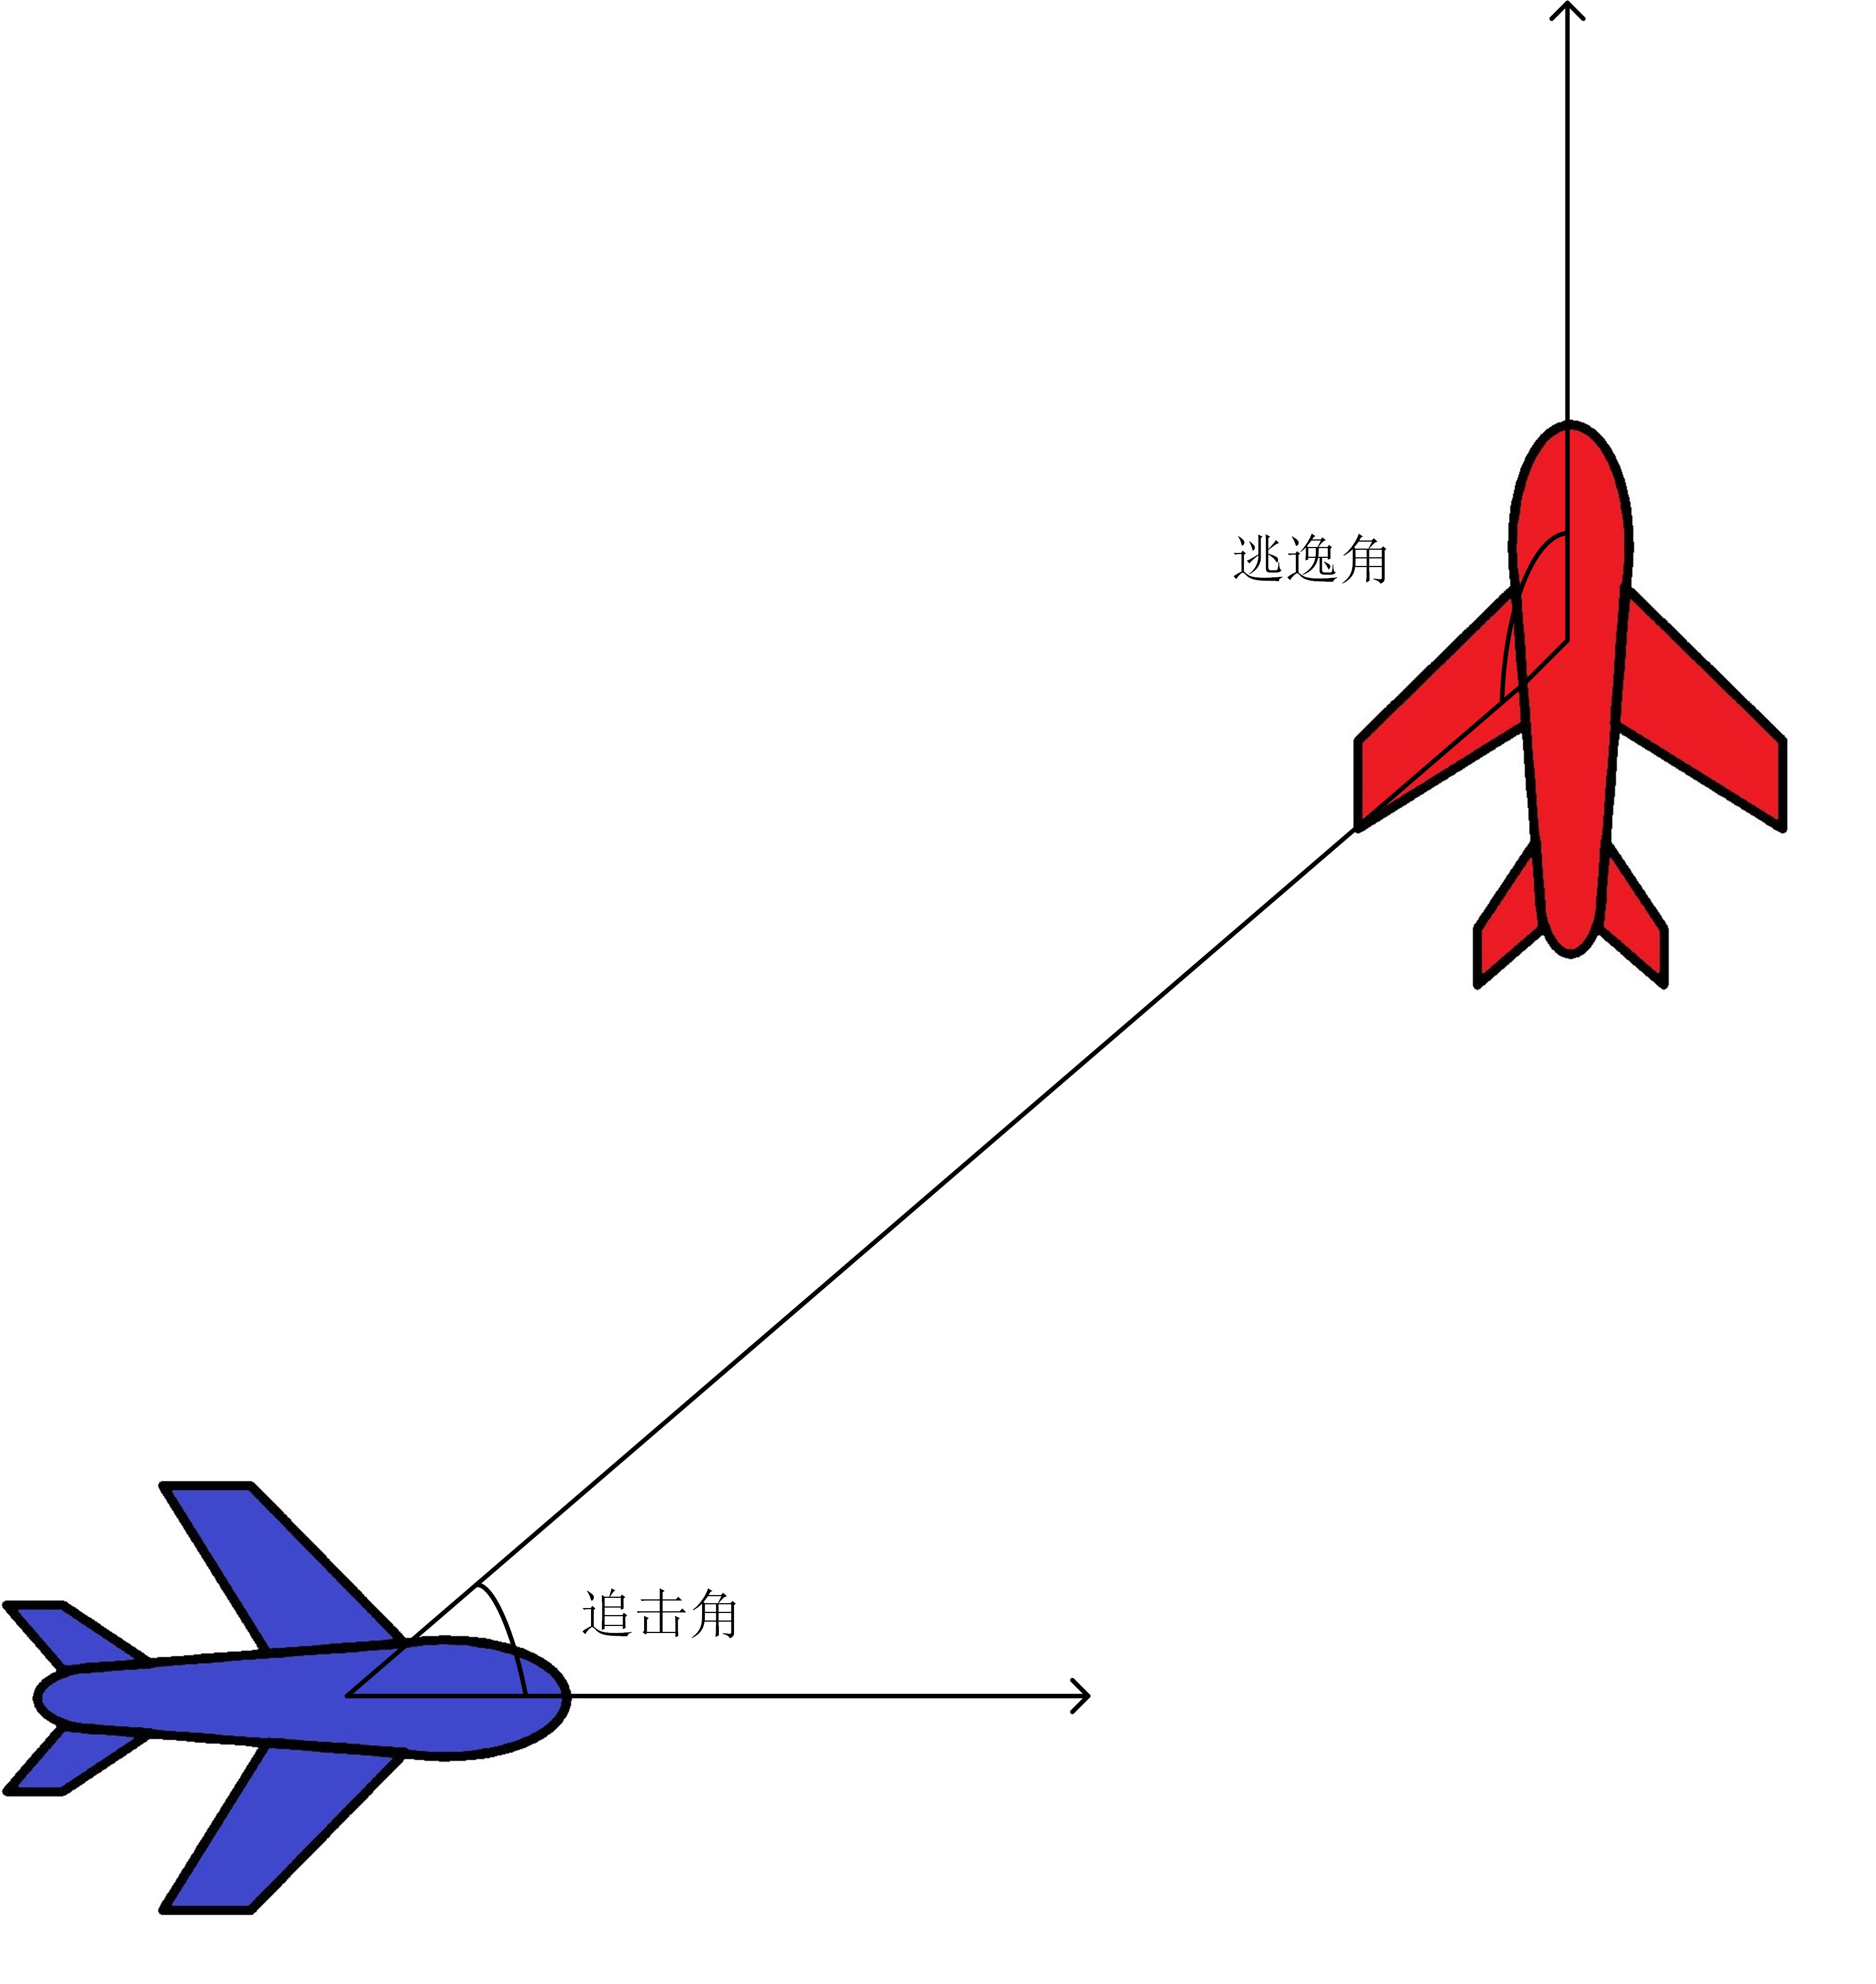
\includegraphics[width=7cm]{example/zhuijijiao.jpg}
	\bicaption[追击角和逃逸角示意图]
	{追击角和逃逸角示意图}
	{Neural network training pipeline}
	\label{fig:zhuijijiao}
\end{figure}

红方击灭蓝方的规则如下:红方到蓝方距离小于四个单位长度,红方的追击角小于$30^\circ$,蓝方的逃逸角大于$30^\circ$。反之蓝方对红方追击角小于$30^\circ$,红方逃逸角大于$30^\circ$,蓝方击灭红方,最后留下的一方获胜。

\subsection{场景建模}
在强化学习框架下,需要对状态空间,动作空间以及奖励函数进行合理表示。为了拟合价值函数和策略函数需要用到深度学习网络,这部分涉及网络结构的设计,激活函数的选择和损失函数的设计。由于是经典的零和博弈模型,动作空间是离散的,树结构可以完整的表示利用强化学习指导飞机对战的过程。这里采用蒙特卡洛搜索树进行建模,需要把强化学习算法映射到蒙特卡洛搜索树的结构上,包括根节点和分支包含的价值和概率函数以及叶子节点返回的值。

在状态空间表示上,首先从游戏规则考虑,游戏获胜的条件和速度方向以及双方的位置信息有关,所以特征平面需要涵盖相关信息,在这里选择5层的$10 \times 10$的特征空间表示状态信息,第一层为我方当前的位置,第二层为我方上一步的位置,第三层为敌方当前位置,第四层为敌方上一步位置,第五层用来标识当前玩家,红方为全0,蓝方为全1。

在动作选择上,飞机移动的位置只能是相连的上下左右四个方向,所以动作空间为4个离散的值。当飞到战场边界时,当前动作认为是非法的。这里我们定义了严格的获胜条件,所以奖励函数比较明确。返回的奖励函数为获胜一方的奖励为1,失败一方奖励为-1。当两方各自走过的步数超过200步还没有分出胜负,判定为平局,奖励为0。

在网络结构上,状态空间时包含了敌方的位置以及动作信息,所以价值网络和策略网络可以利用相同的网络结构进行特征提取,把经过CNN网络进行特征提取后的数据分别接入不同的全连接网络。策略网络输出的是各个动作的概率信息可以看成4分类的问题,所以接入softmax函数,价值网络是一个回归问题,接入tanh函数基于当前的状态和动作对最后的预测结果进行回归。深度学习的网络设置如表\ref{tab4}所示。

\begin{table}[htbp]
	\centering
	\bicaption[一对一深度学习网络参数]
	{一对一深度学习网络参数}
	{ Deep learning network parameters }
	\label{tab4}
	\begin{tabular}{llll} \toprule
		网络名称   & 网络结构  \\  \midrule
		特征提取 &	Conv2d(4, 32, kernel\_size=3, padding=1), ReLU\\
		&	Conv2d(32, 64, kernel\_size=3, padding=1),ReLU\\
		&	Conv2d(64, 128, kernel\_size=3, padding=1), ReLU\\
		价值网络&Conv2d(128, 2, kernel\_size=1), ReLU\\
		&Linear(2*board\_width*board\_height, 64), ReLU\\
		&Linear(64, 1),tanh\\
		策略网络&12 Conv2d(128, 4, kernel\_size=1), ReLU\\
		&Linear(4*board\_width*board\_height,
		4),softmax\\
		
		\bottomrule
	\end{tabular}
\end{table}


\subsection{一对一实验结果与分析}
本节将就一对一智能体博弈模型进行结果展示和分析。在这里参数设置为当每进行一次动作选择,对当前状态进行400次蒙特卡洛树搜索统计搜索结果。根据每个节点的访问次数利用式\ref{eq:gailu}和式\ref{eq:zaosheng}进行节点信息统计得到当前状态的动作。这里面选取温度常数$\tau=1$,噪声系数$\varepsilon=0.25$,学习率调整参数为$\lambda=1.5$。在每一次蒙特卡洛树的搜索和建立中,对于当前位置可选的动作有上下左右,当智能体在作战边界时,会把不能移动的动作去掉,根据可行动作进行树的节点扩展。对于当前智能体的子节点扩展就是对方可行的动作。在动作选择时,选取最大的$Q+U$进行动作的选择,这里$Q$代表经过当前节点获得的平均奖励,$U$为根据深度学习网络得到的先验概率。

红蓝两方初始位置分别为$(2,3)$和$(7,7)$,红方初速度为向上,蓝方初速度为向下。人类控制红方,蓝方为AI。红蓝两方的初始状态如图\ref{fig1:yiduiyi1-2:a}所示。红方为先行玩家,动作向右后得到蓝方的动作概率,如图\ref{fig1:yiduiyi1-2:b}。


\begin{figure}[htpb]
	\centering
	\subcaptionbox{\label{fig1:yiduiyi1-2:a}}
	{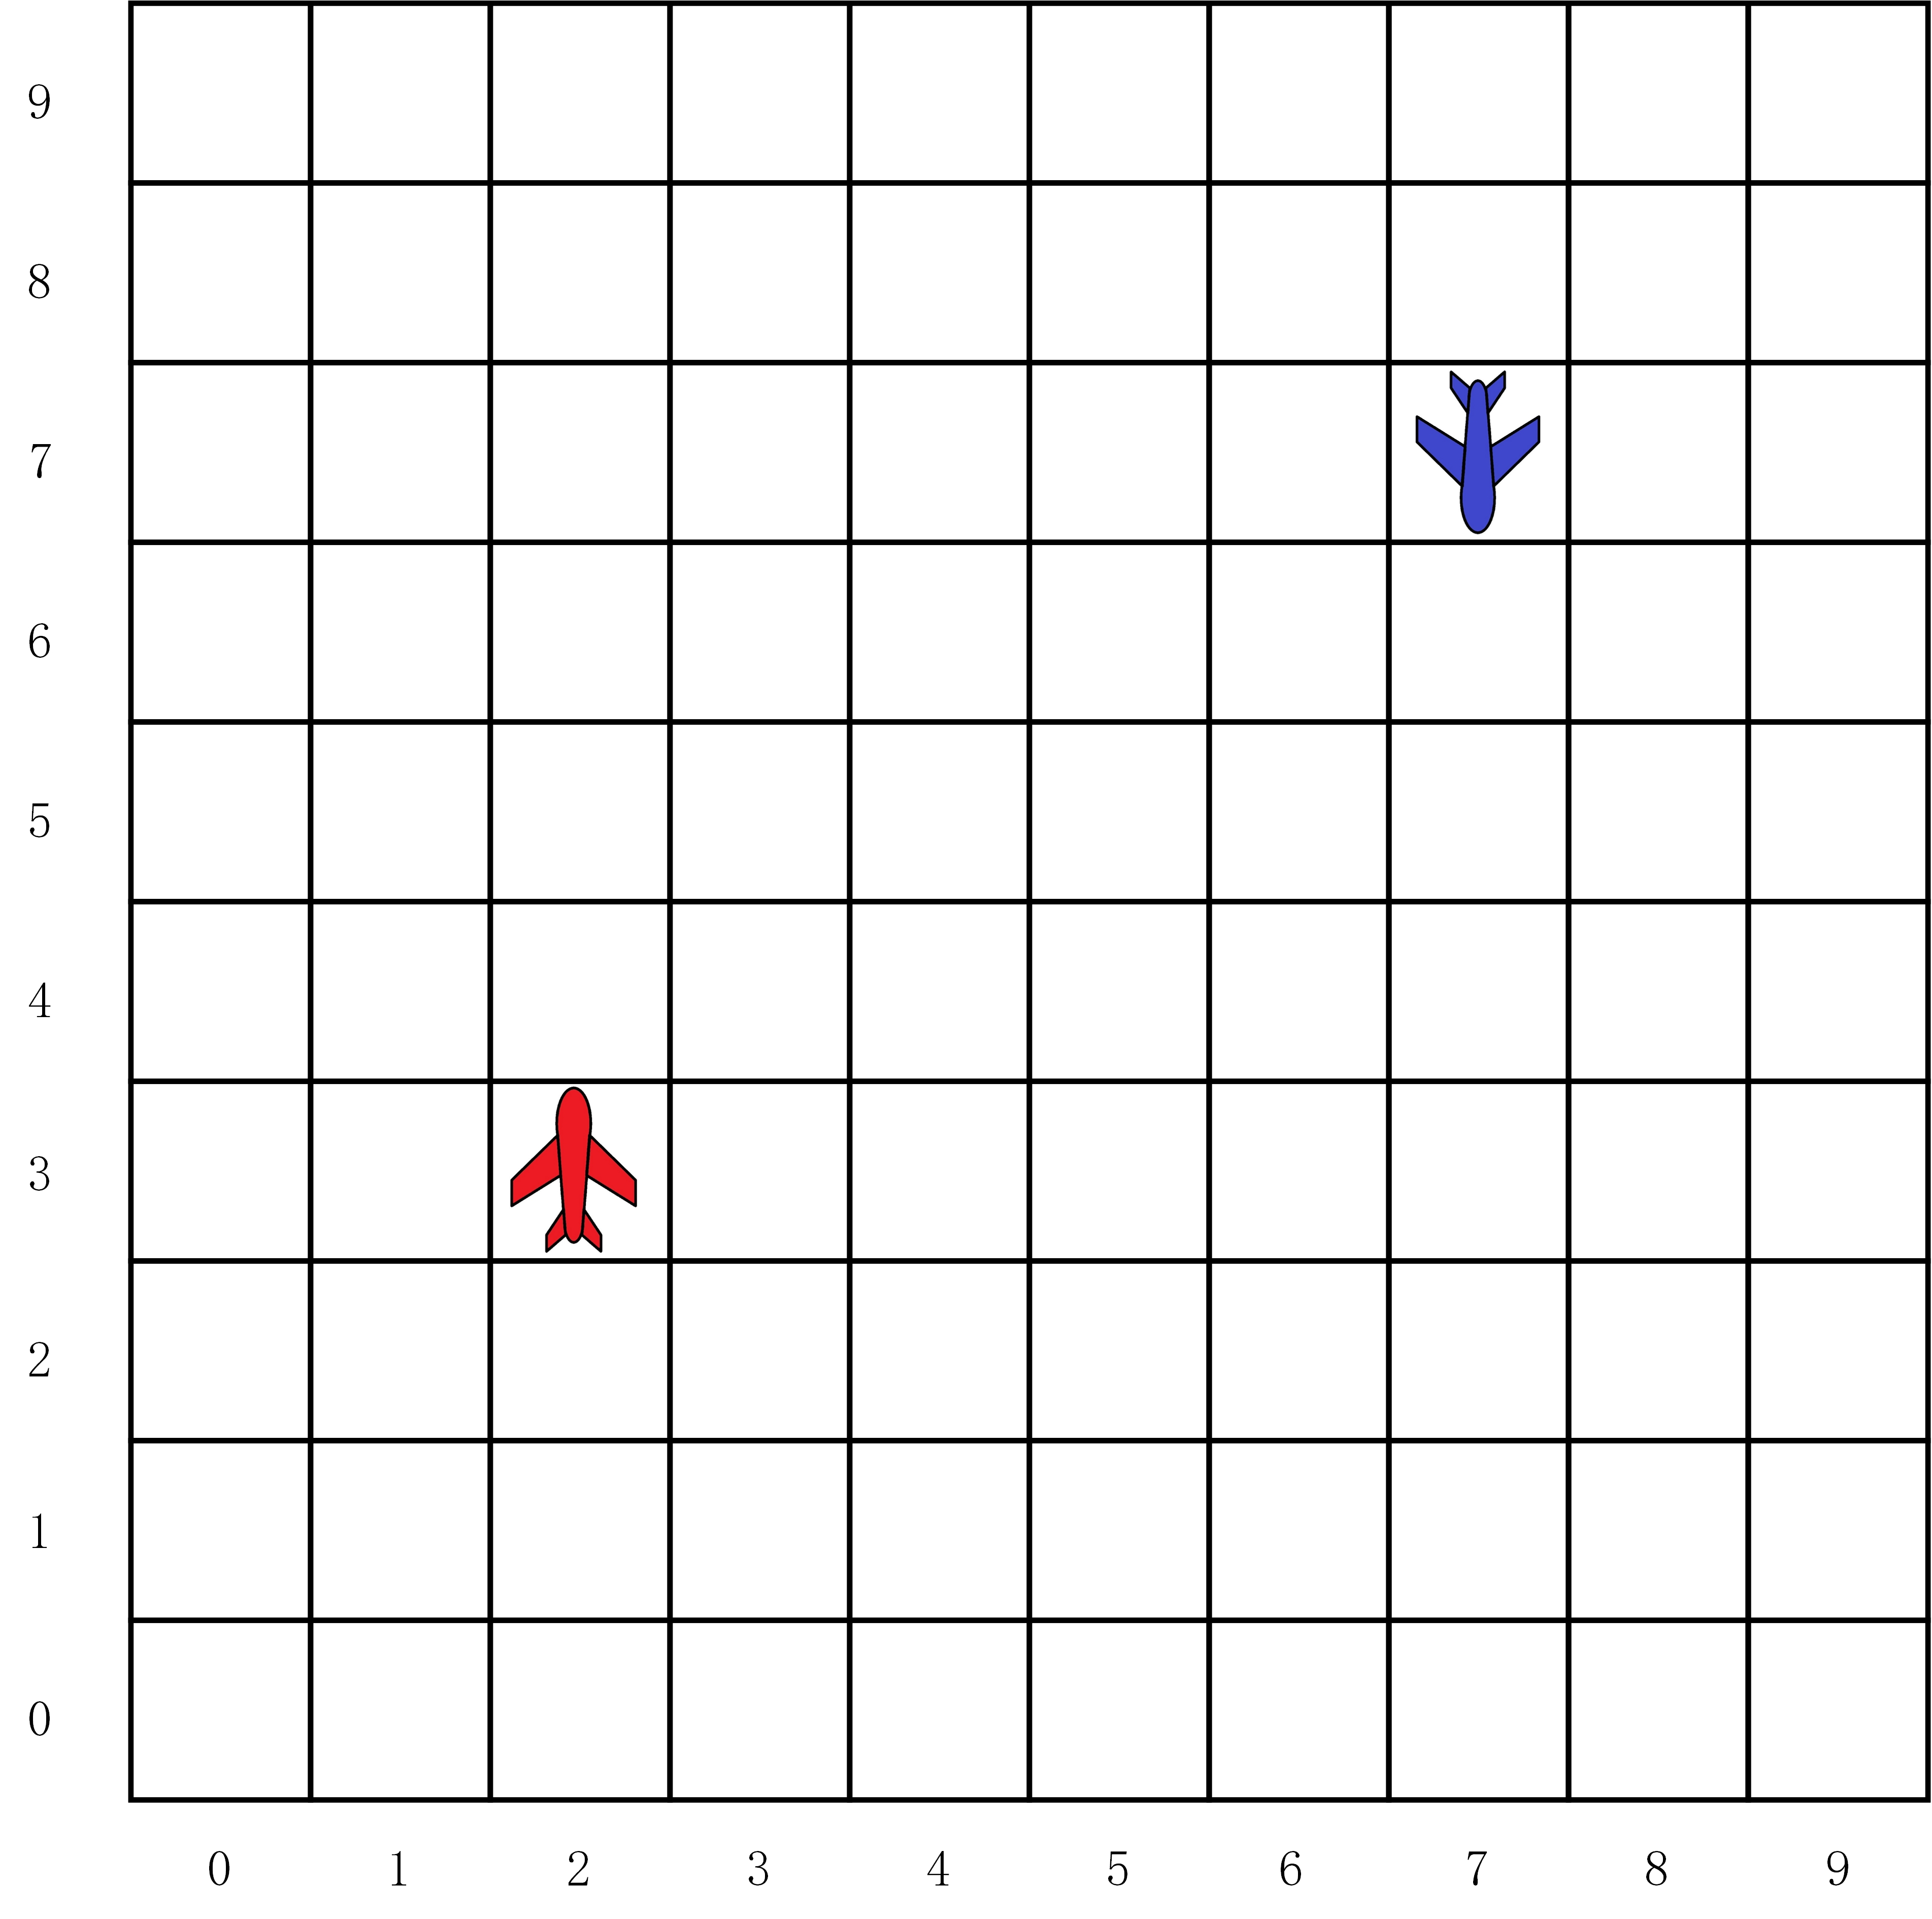
\includegraphics[width=0.45\hsize,height=0.45\hsize]{example/feijiyiduiyi1.jpg}}
	\subcaptionbox{\label{fig1:yiduiyi1-2:b}}
	{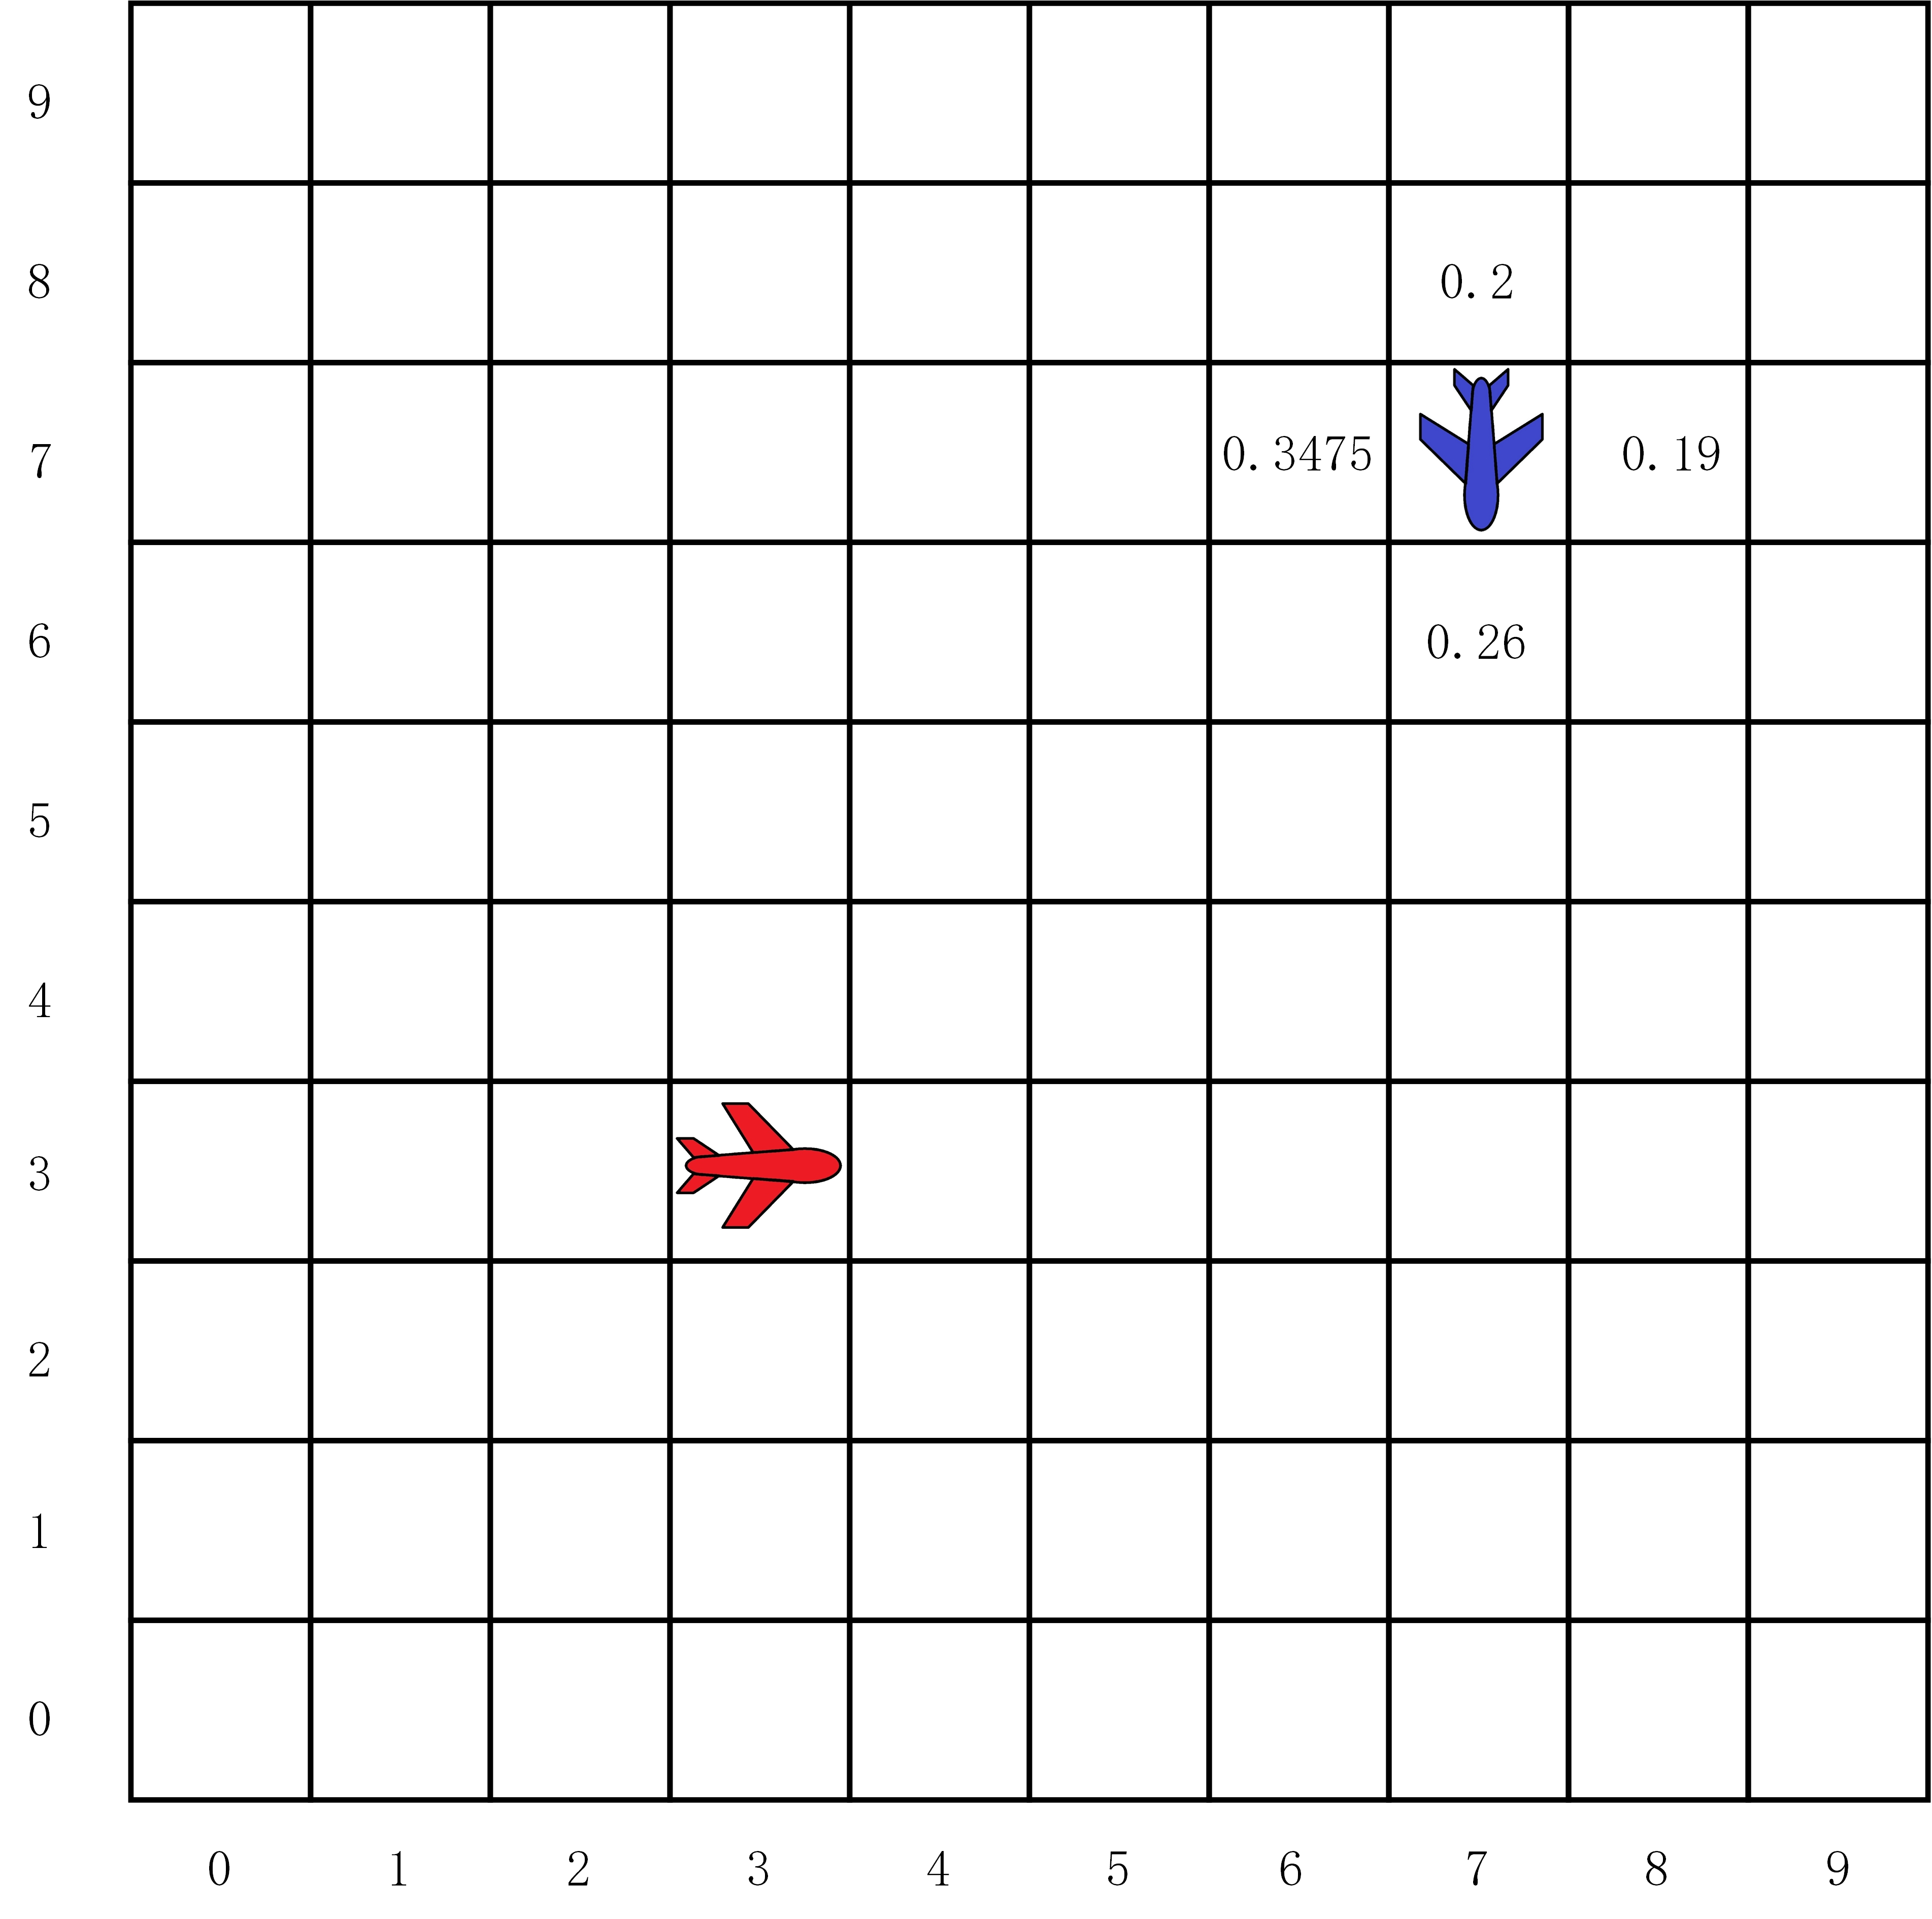
\includegraphics[width=0.45\hsize,height=0.45\hsize]{example/feijiyiduiyi2.jpg}}
	\bicaption
	{红蓝两方初始状态}
	{Initial state of red and blue.}
	\label{fig1:yiduiyi1-2}
\end{figure}


接着蓝方取动作概率中的最大值进行动作,依次循环进行动作选择。人机对弈过程如图\ref{fig2:yiduiyi3-6}。对于图\ref{fig2:yiduiyi3-6:b}状态,假设蓝方分别执行四个动作,分析其和红方的相对状态,如图\ref{fig2:yiduiyi7-10}。

\begin{figure}[htp]
	\centering
	\subcaptionbox{\label{fig2:yiduiyi3-6:a}}
	{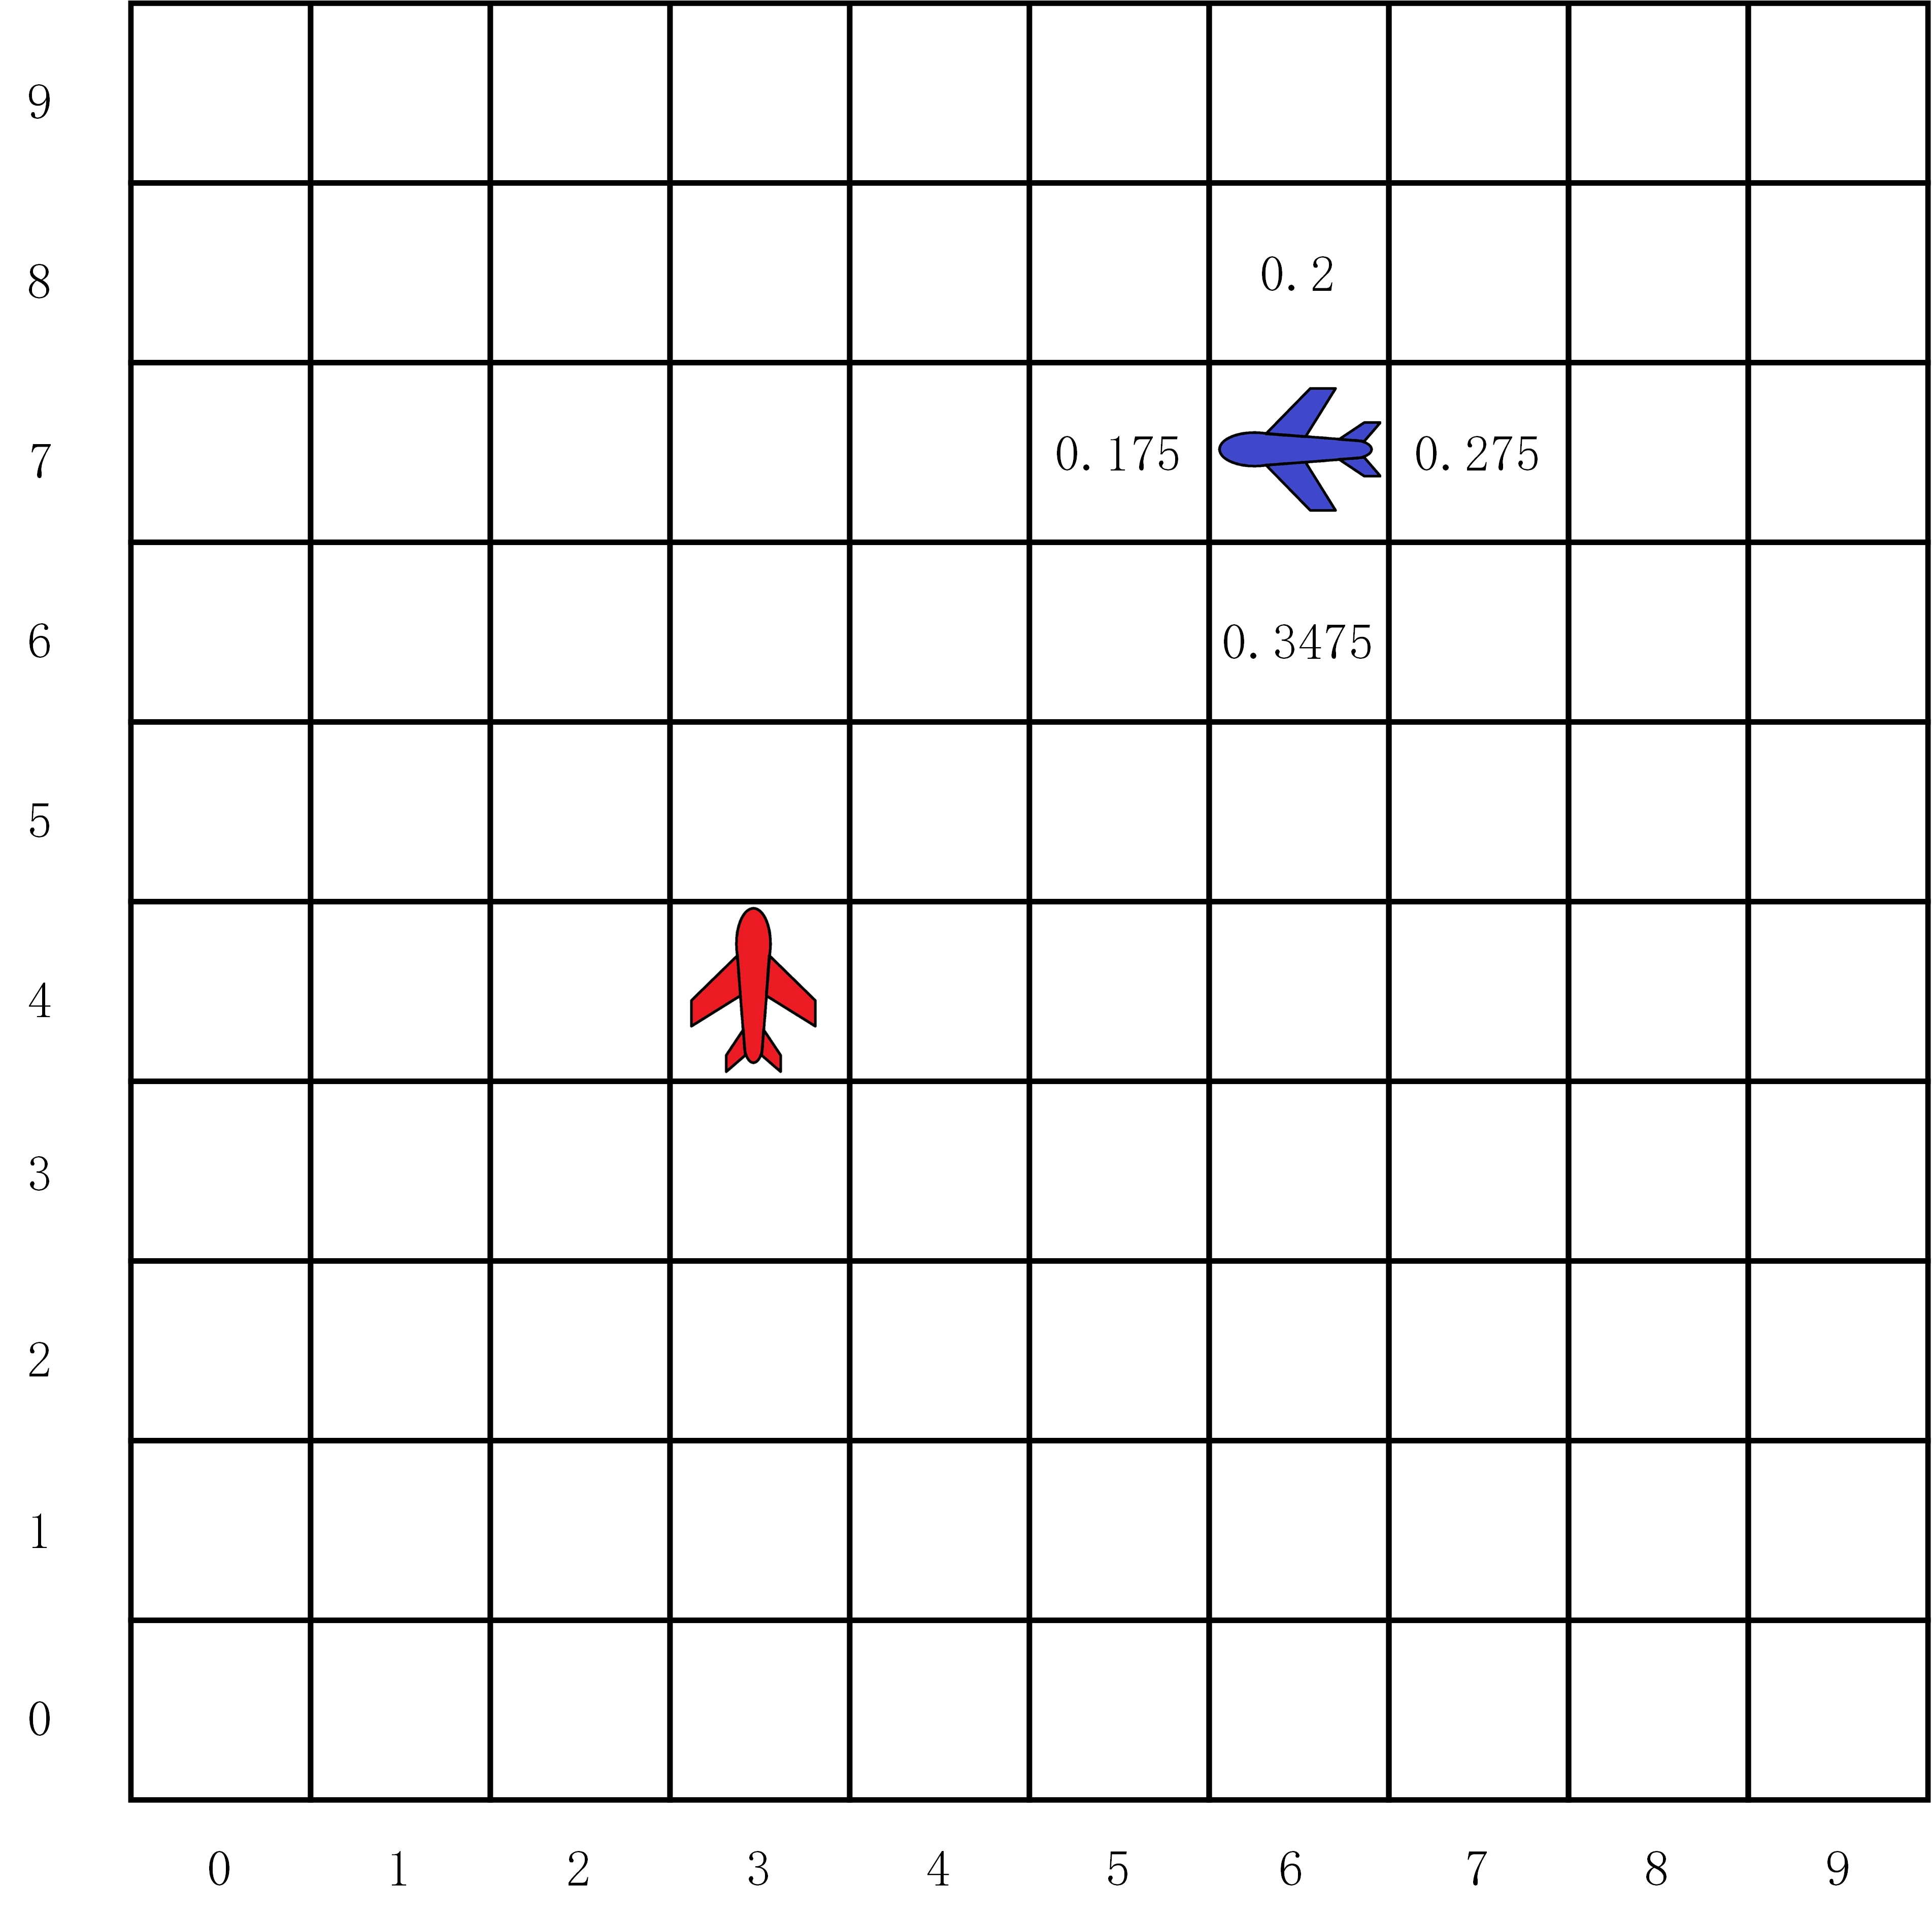
\includegraphics[width=0.45\hsize,height=0.45\hsize]{example/feijiyiduiyi3.jpg}}
	\subcaptionbox{\label{fig2:yiduiyi3-6:b}}
	{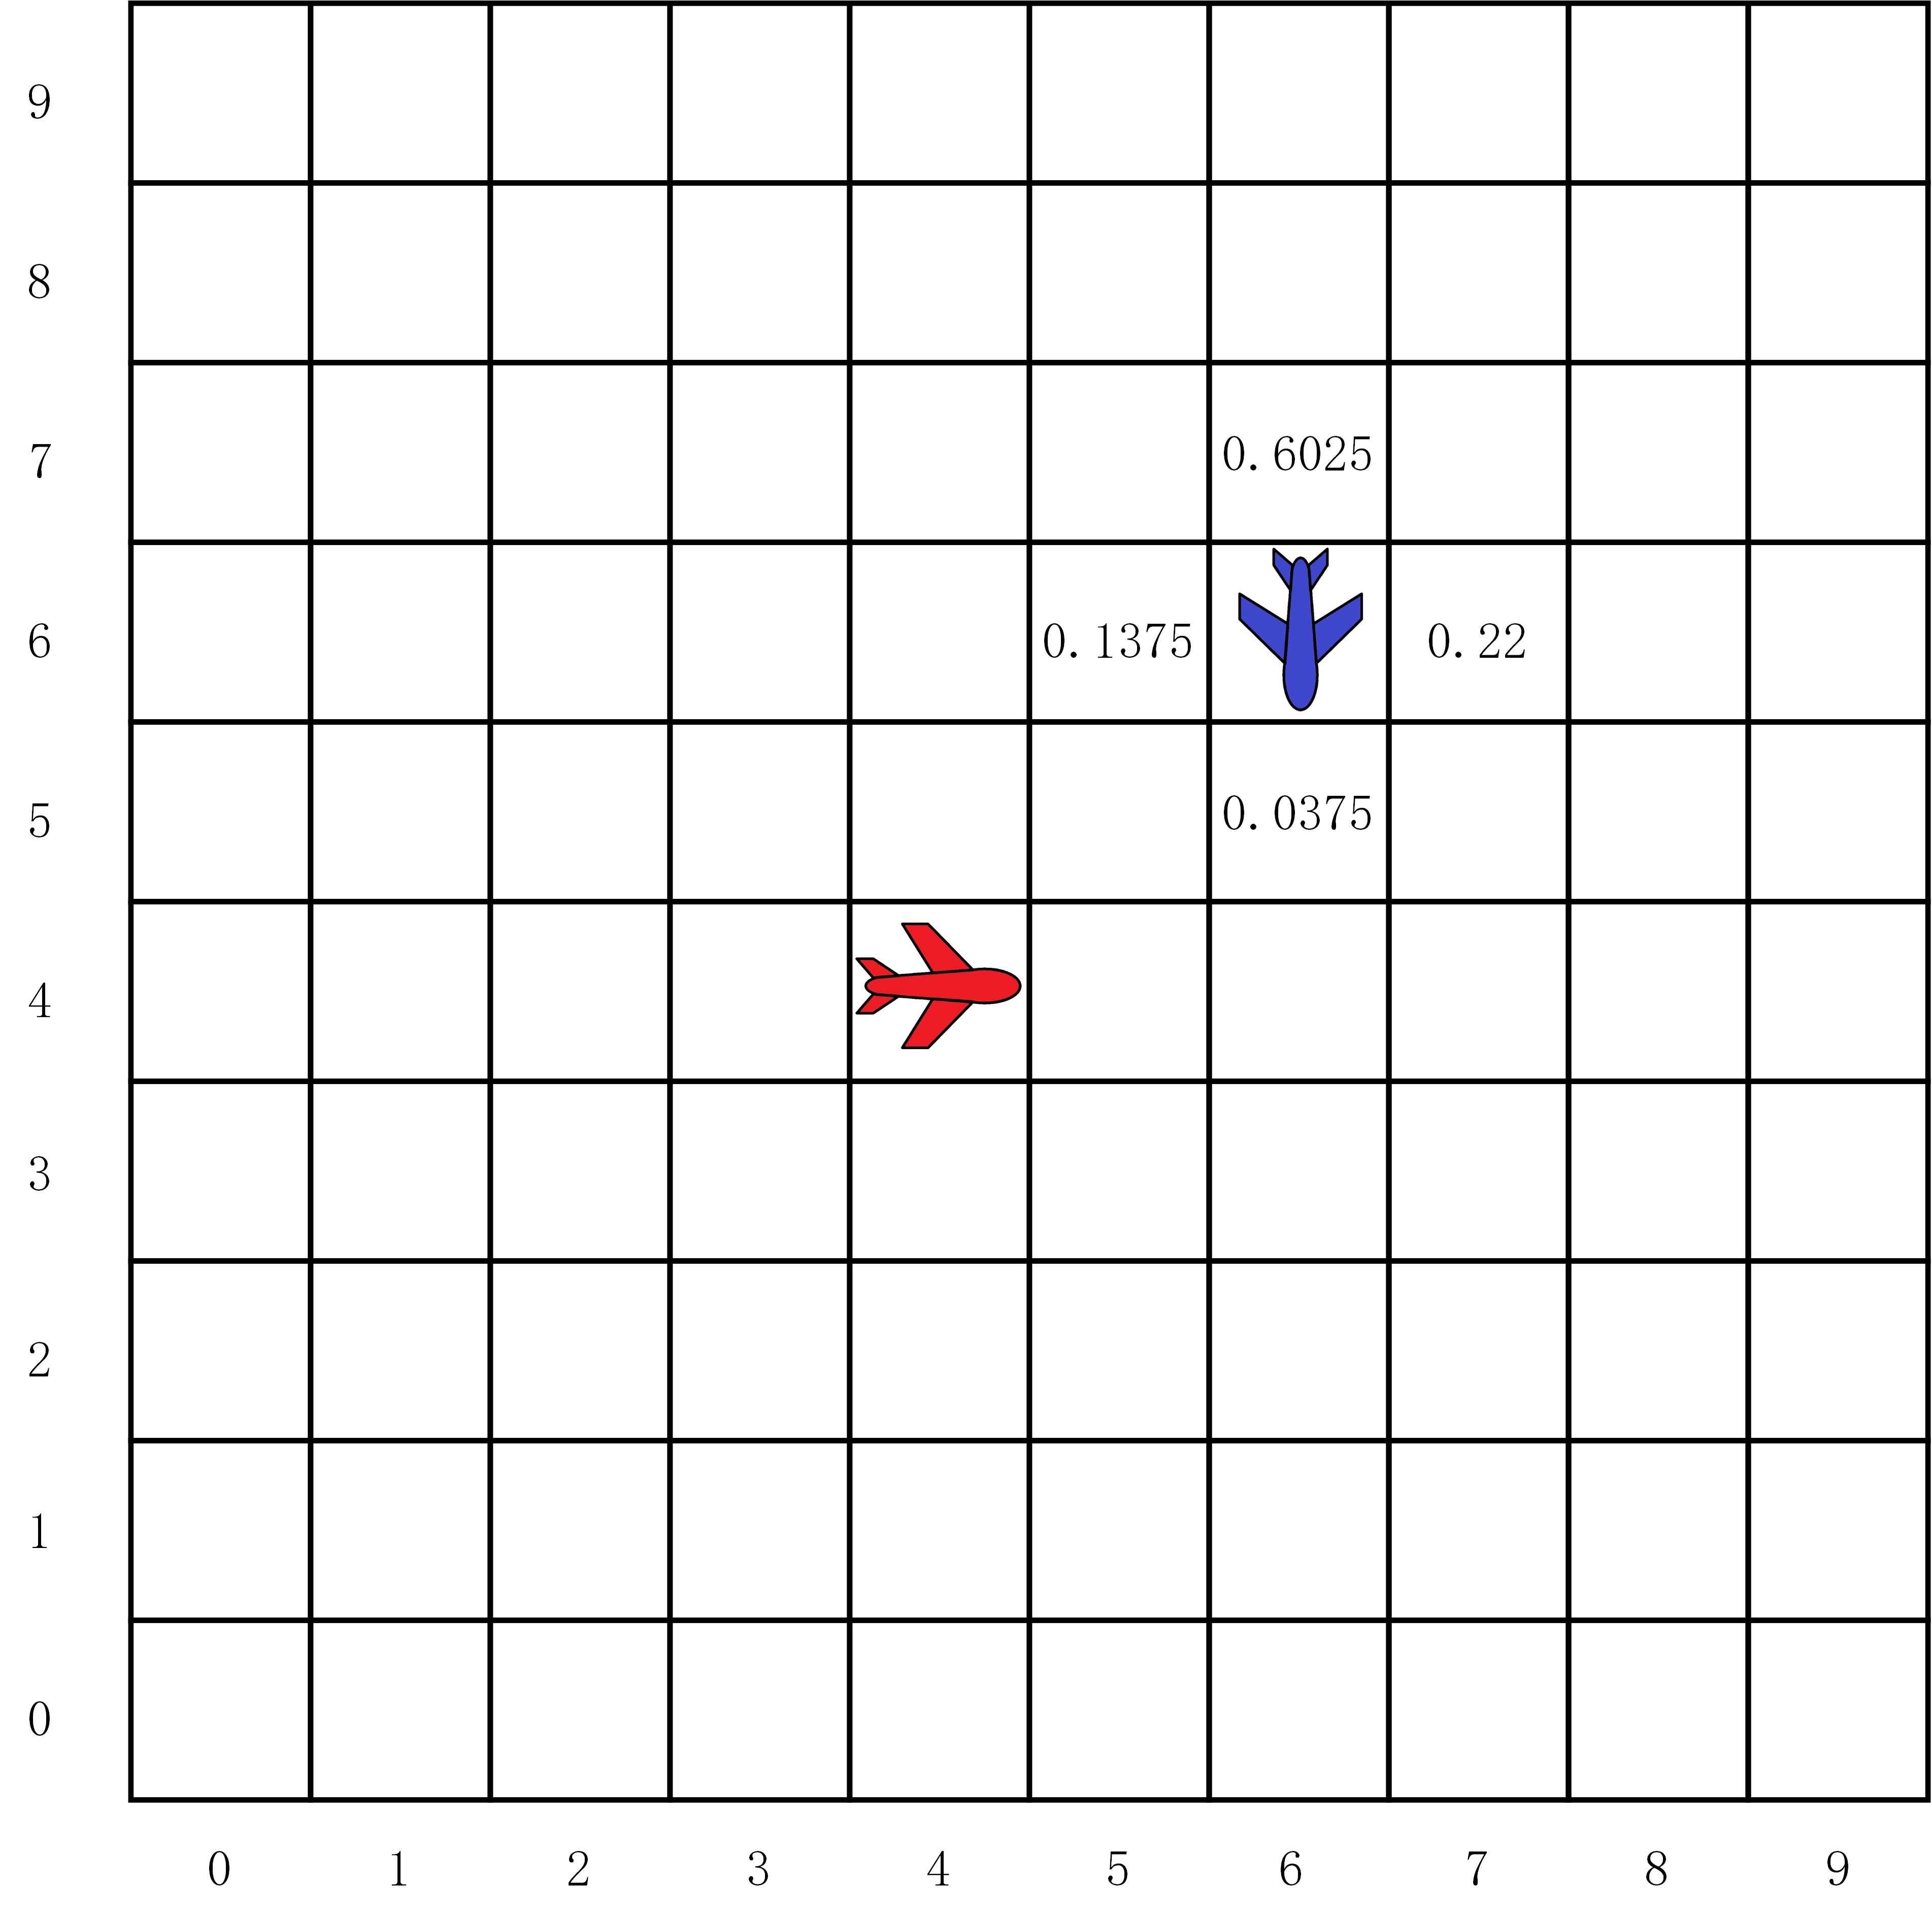
\includegraphics[width=0.45\hsize,height=0.45\hsize]{example/feijiyiduiyi4.jpg}}
	\newline
	\centering
	\subcaptionbox{\label{fig2:yiduiyi3-6:c}}
	{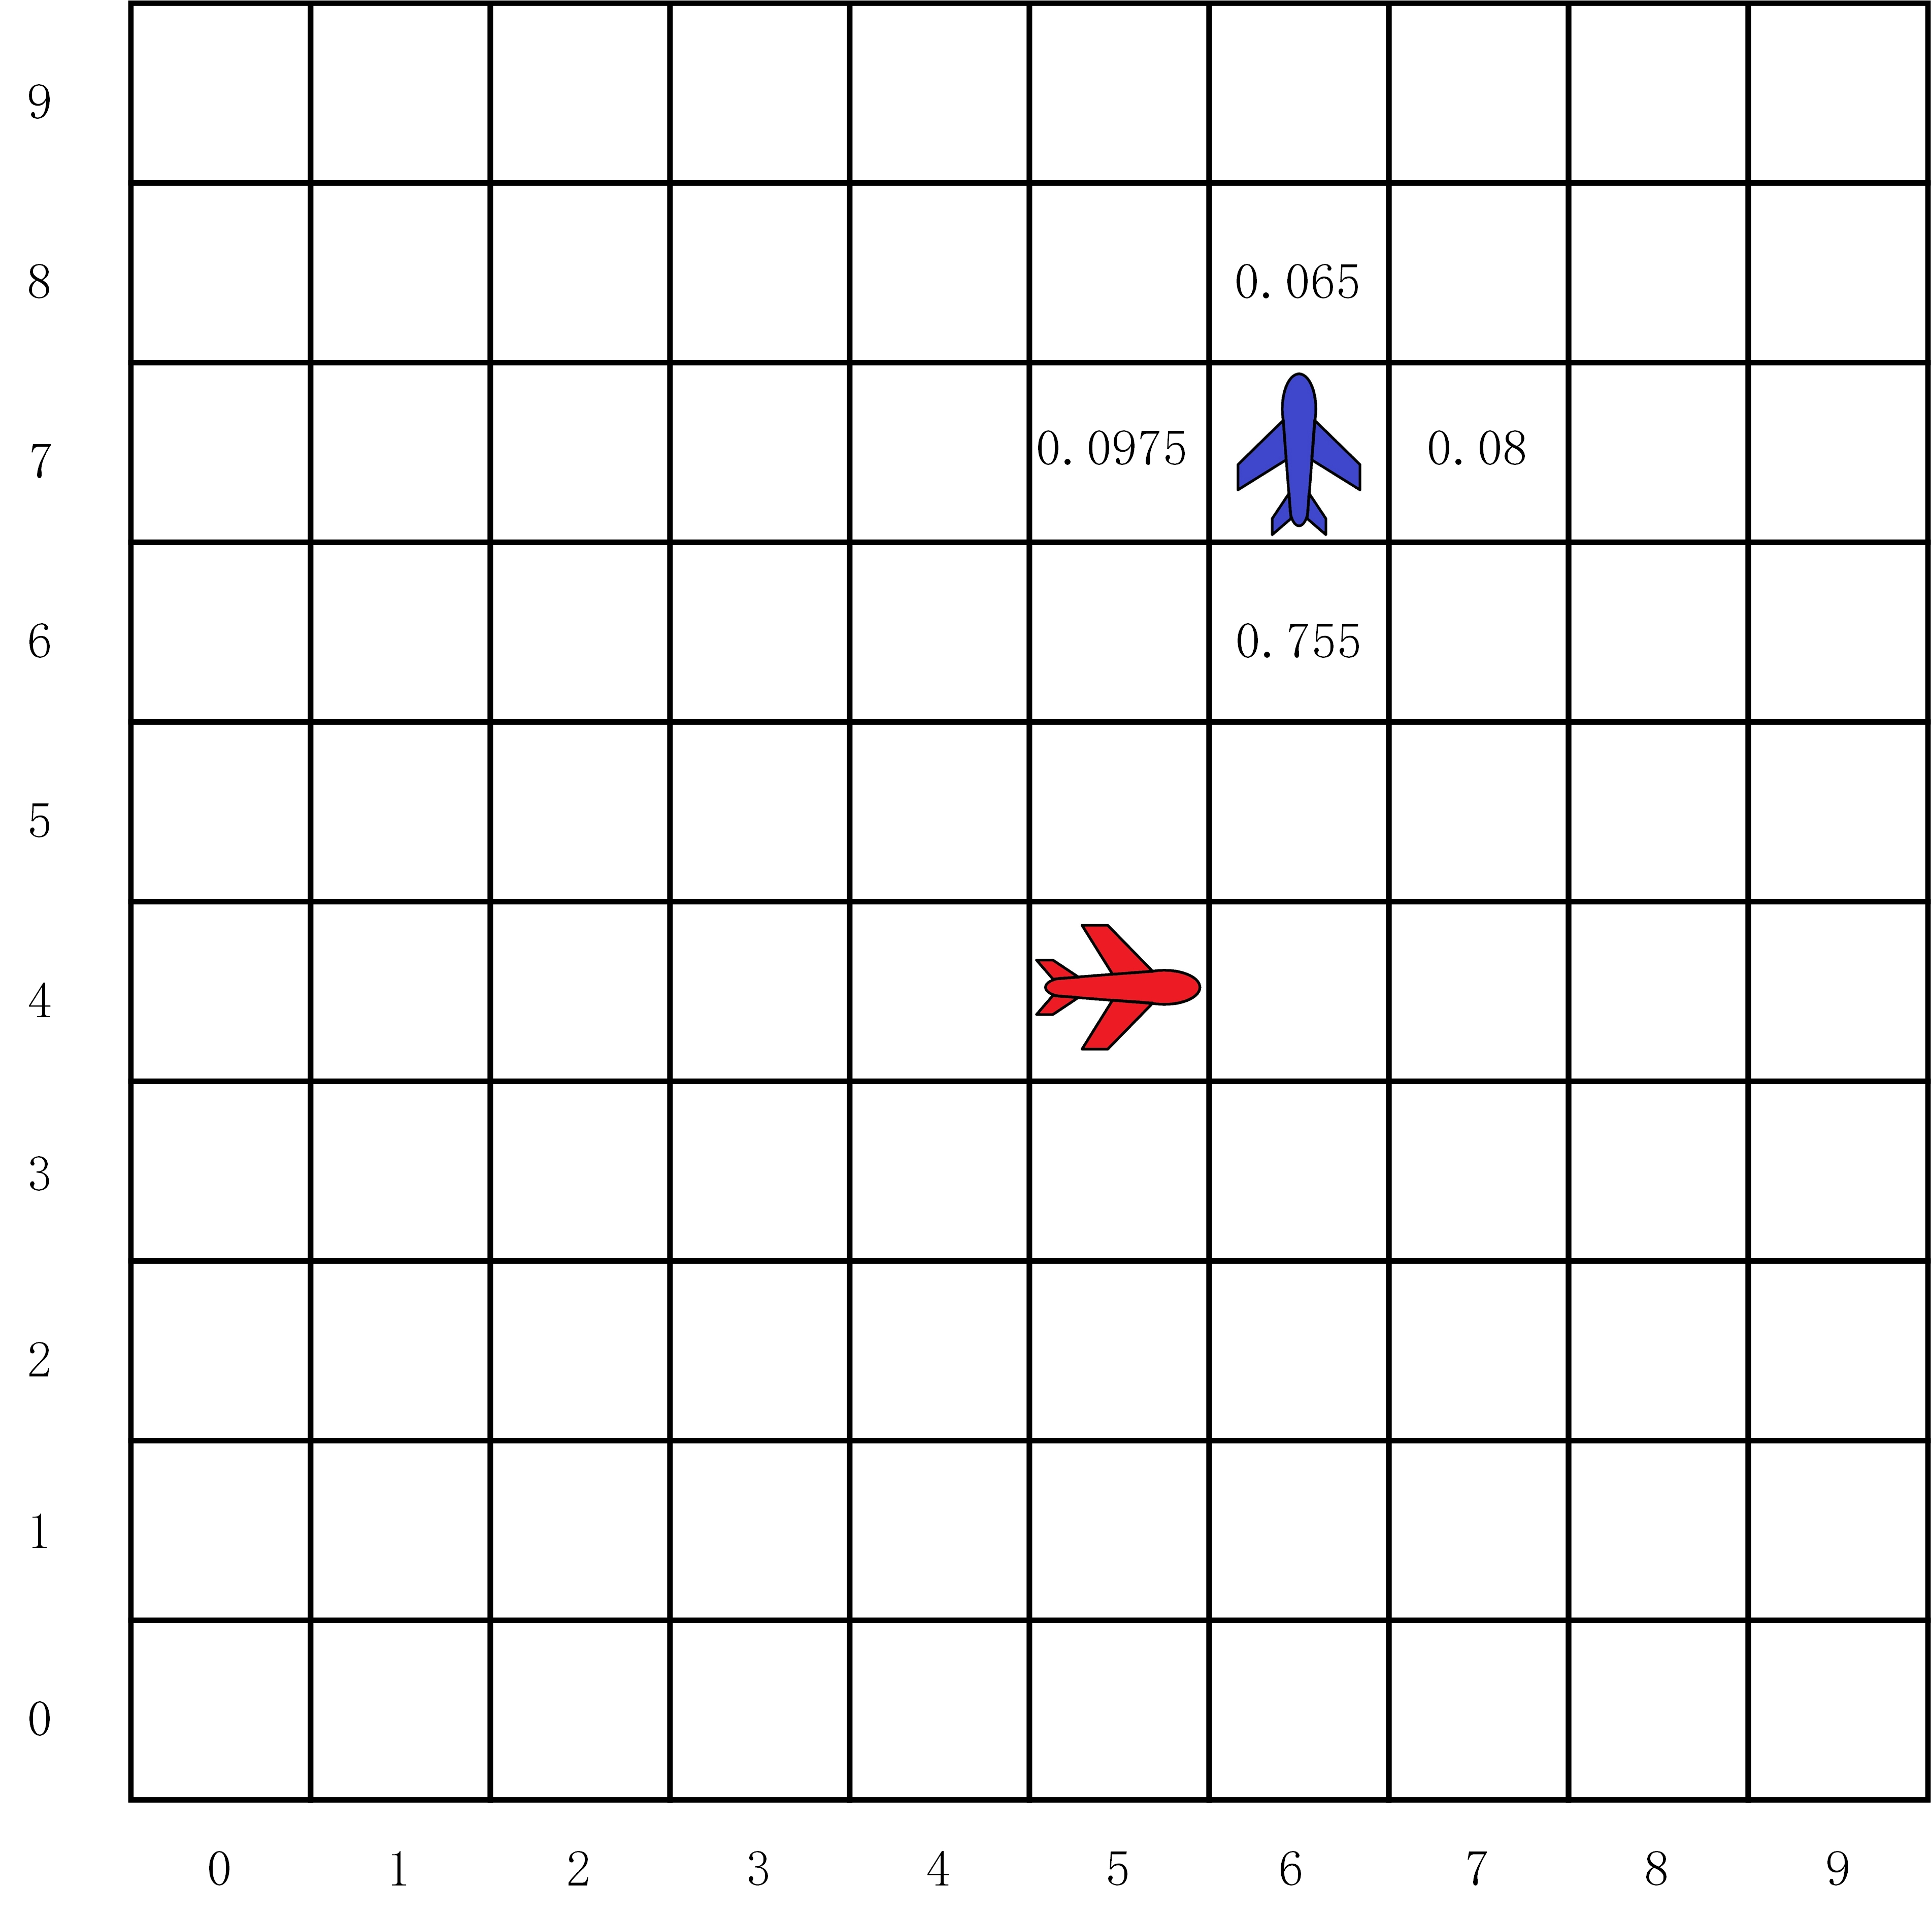
\includegraphics[width=0.45\hsize,height=0.45\hsize]{example/feijiyiduiyi5.jpg}}
	\subcaptionbox{\label{fig2:yiduiyi3-6:d}}
	{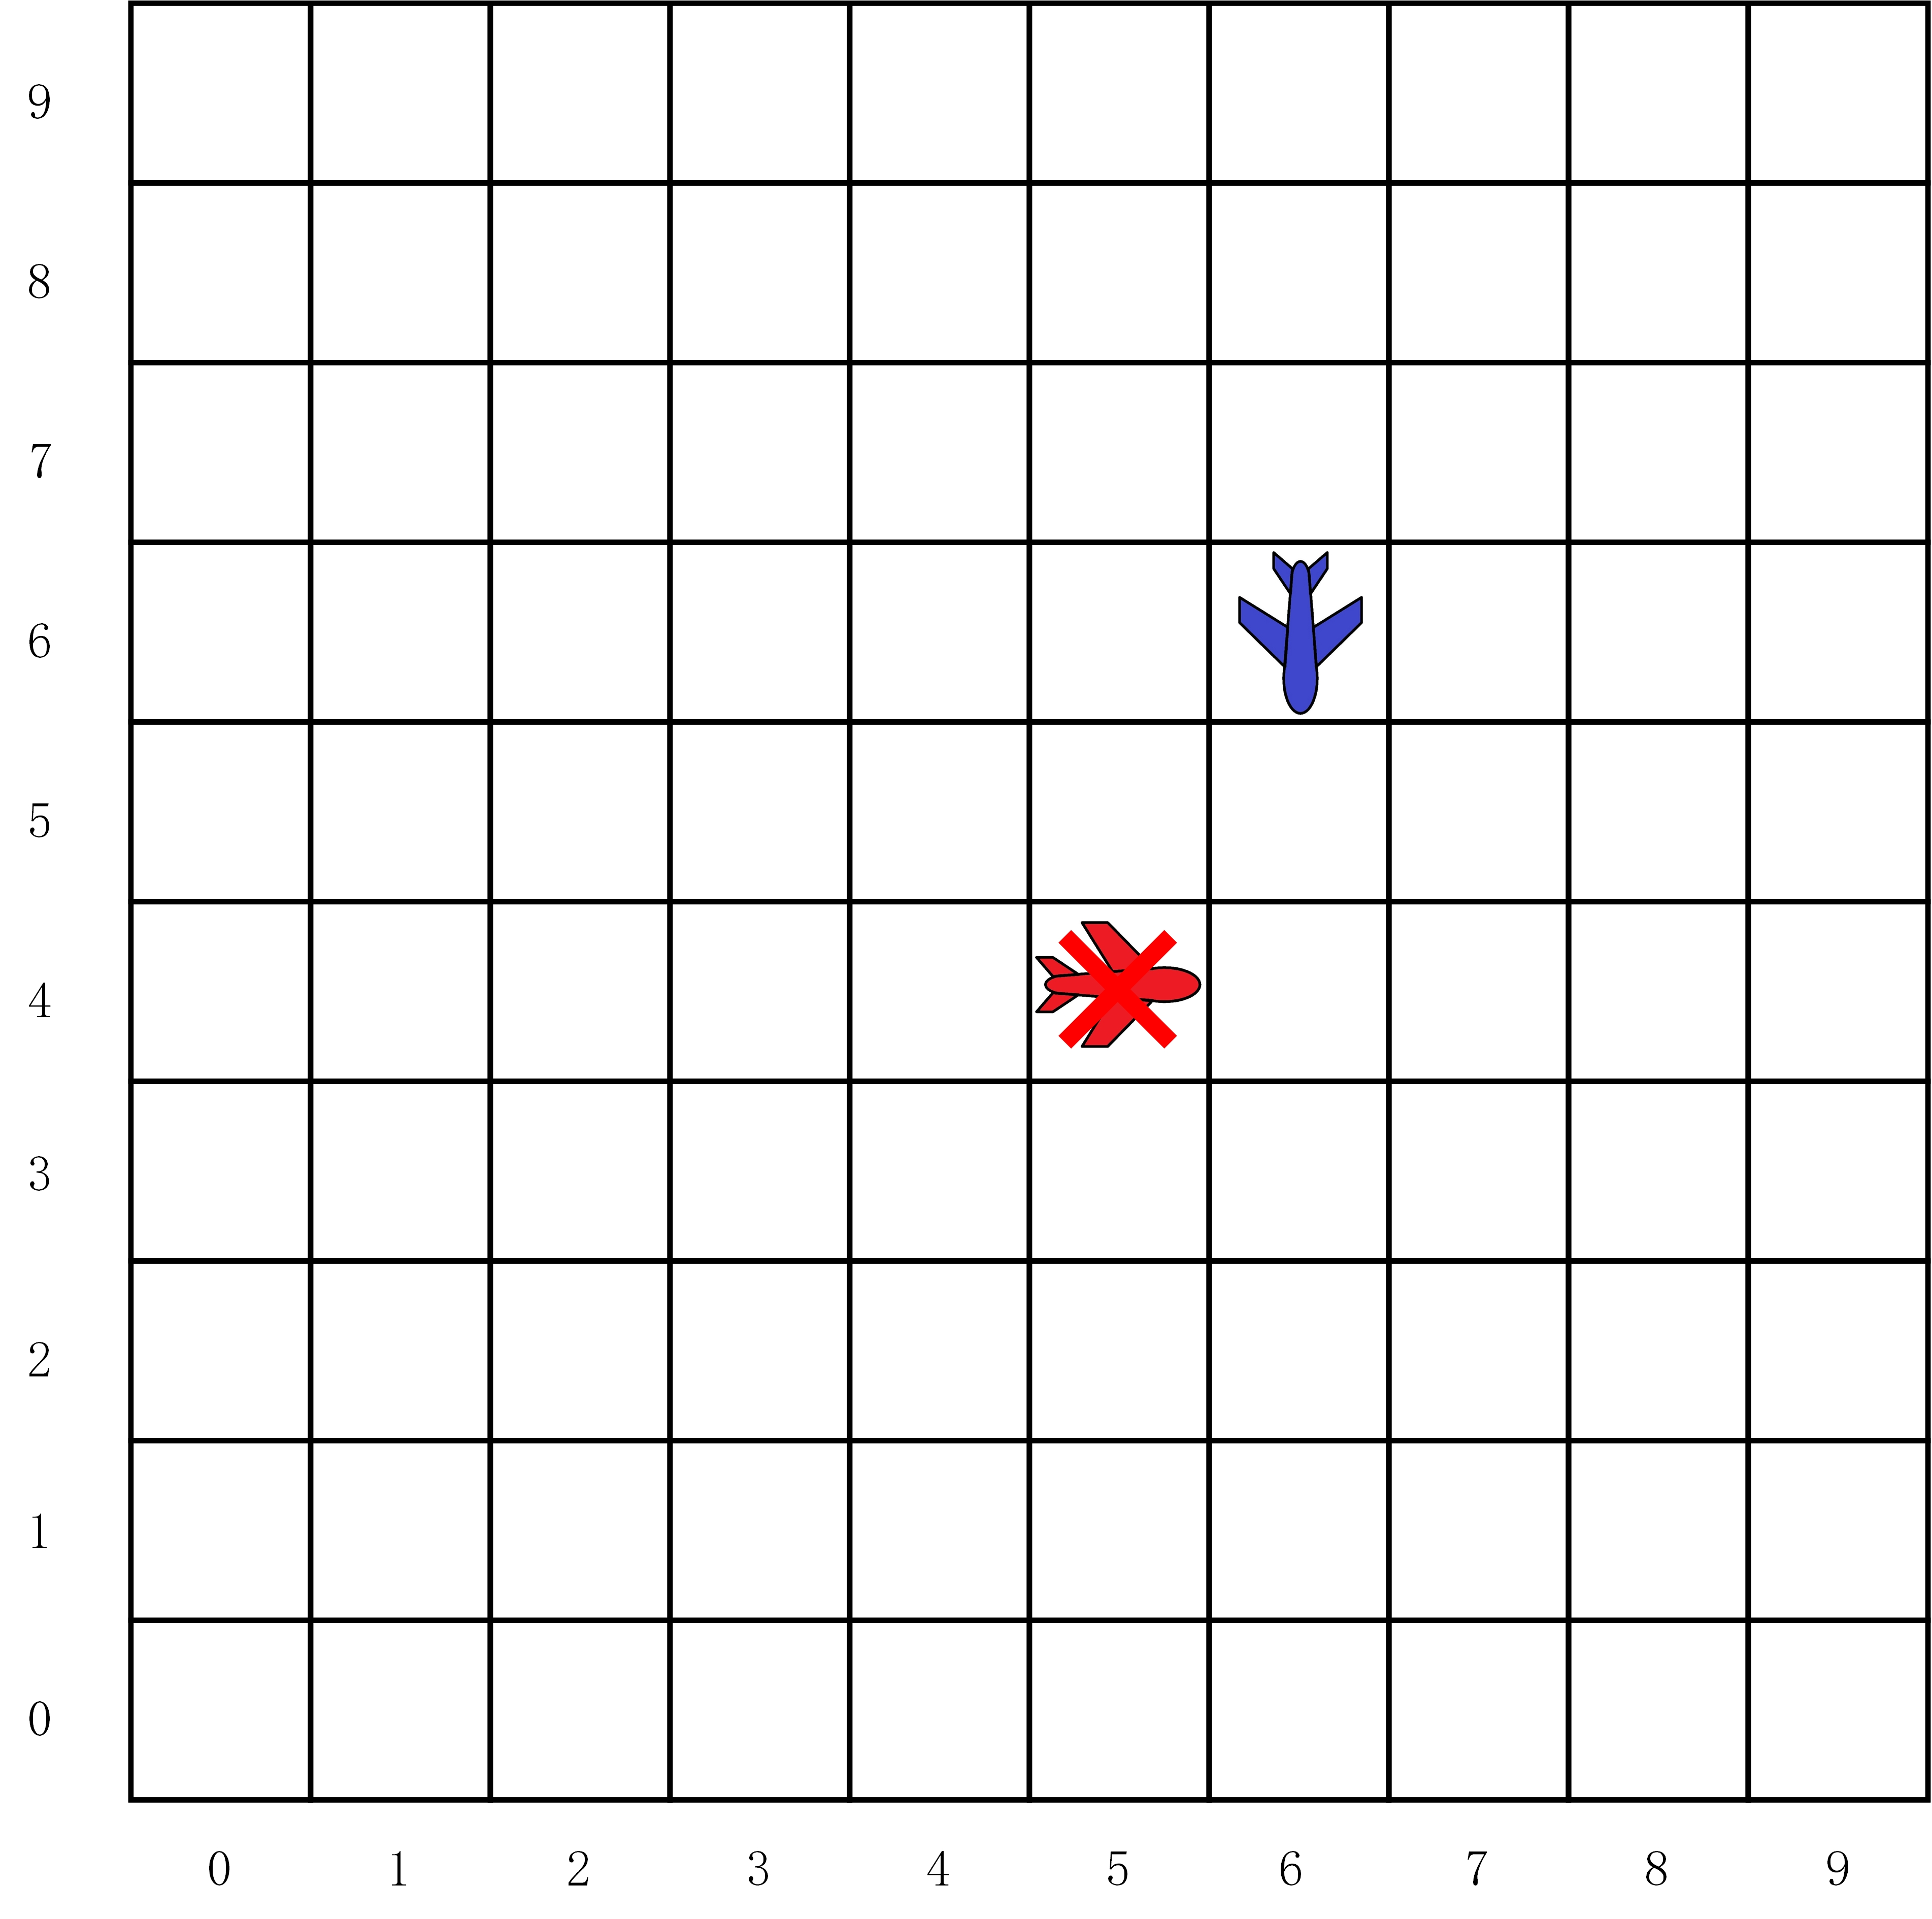
\includegraphics[width=0.45\hsize,height=0.45\hsize]{example/feijiyiduiyi6.jpg}}
	\bicaption
	{一对一人机对弈过程图示}
	{Diagram of one-to-one man-machine game process.}
	\label{fig2:yiduiyi3-6}
\end{figure}


\begin{figure}[htbp]
	\centering
	\subcaptionbox{向上双方状态\label{fig2:yiduiyi7-10:a}}
	{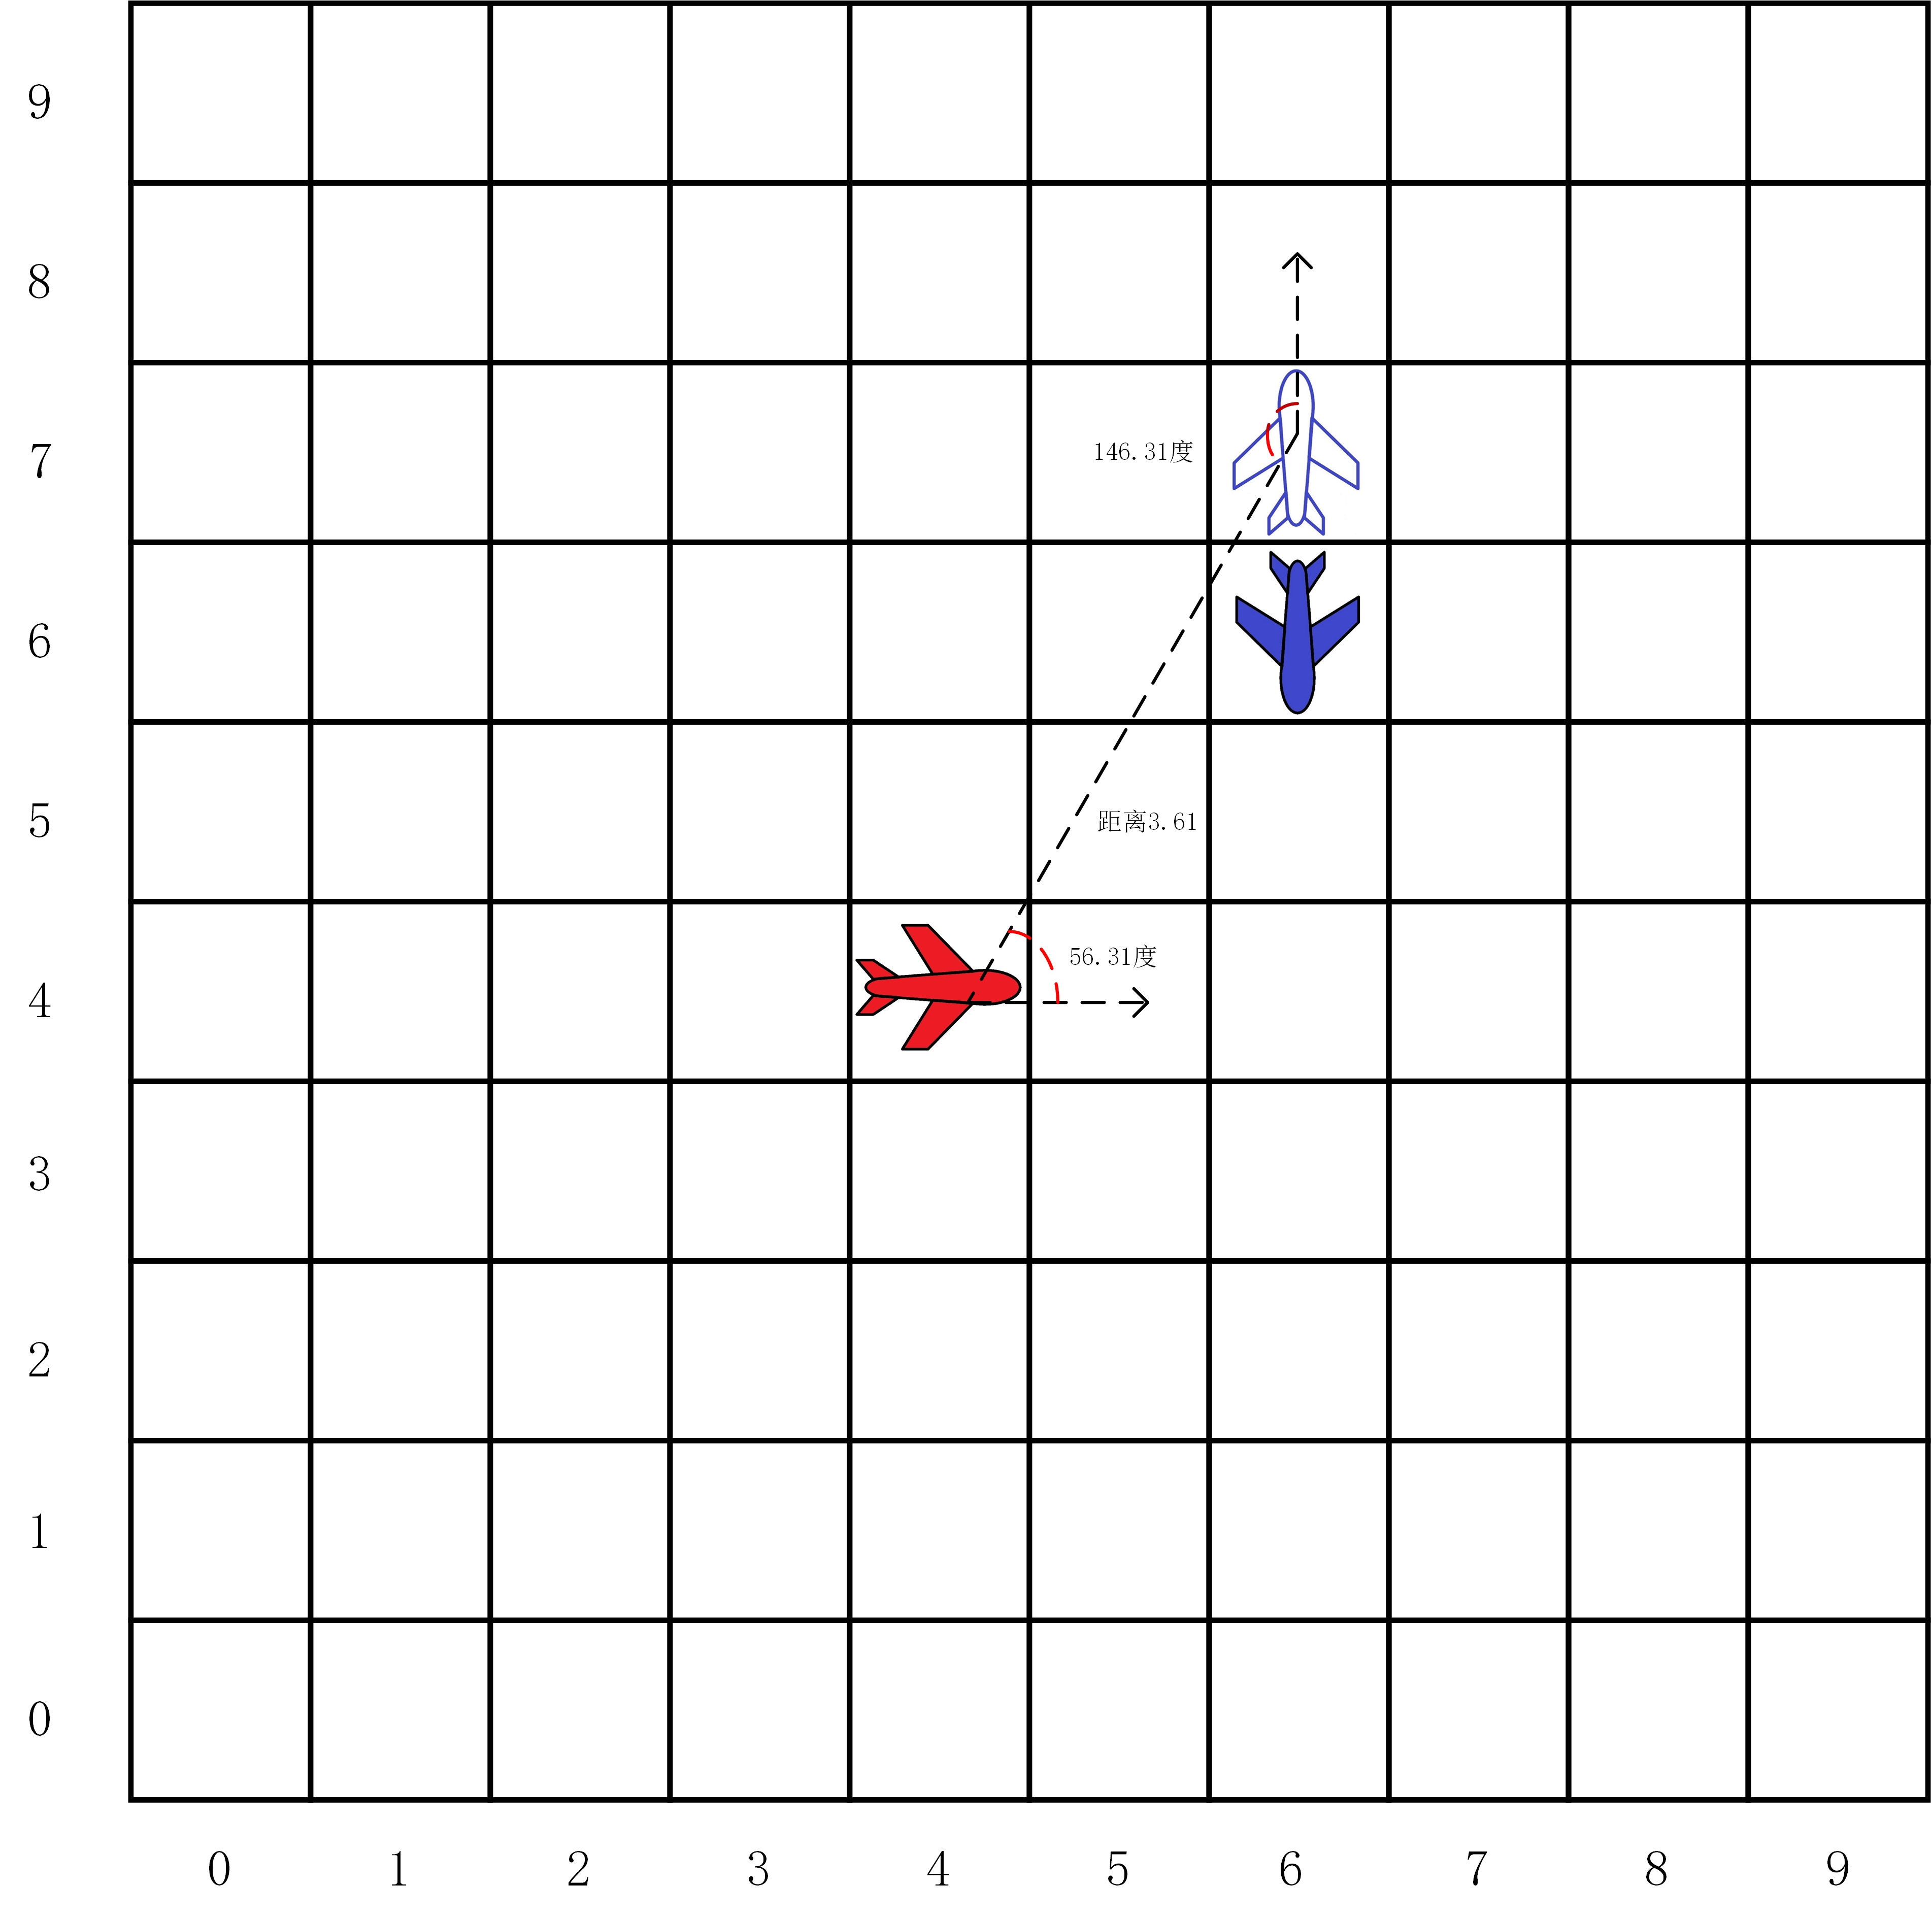
\includegraphics[width=0.45\hsize,height=0.45\hsize]{example/feijiyiduiyi7.jpg}}
	\hspace{0.5em}
	\subcaptionbox{向下双方状态\label{fig2:yiduiyi7-10:b}}
	{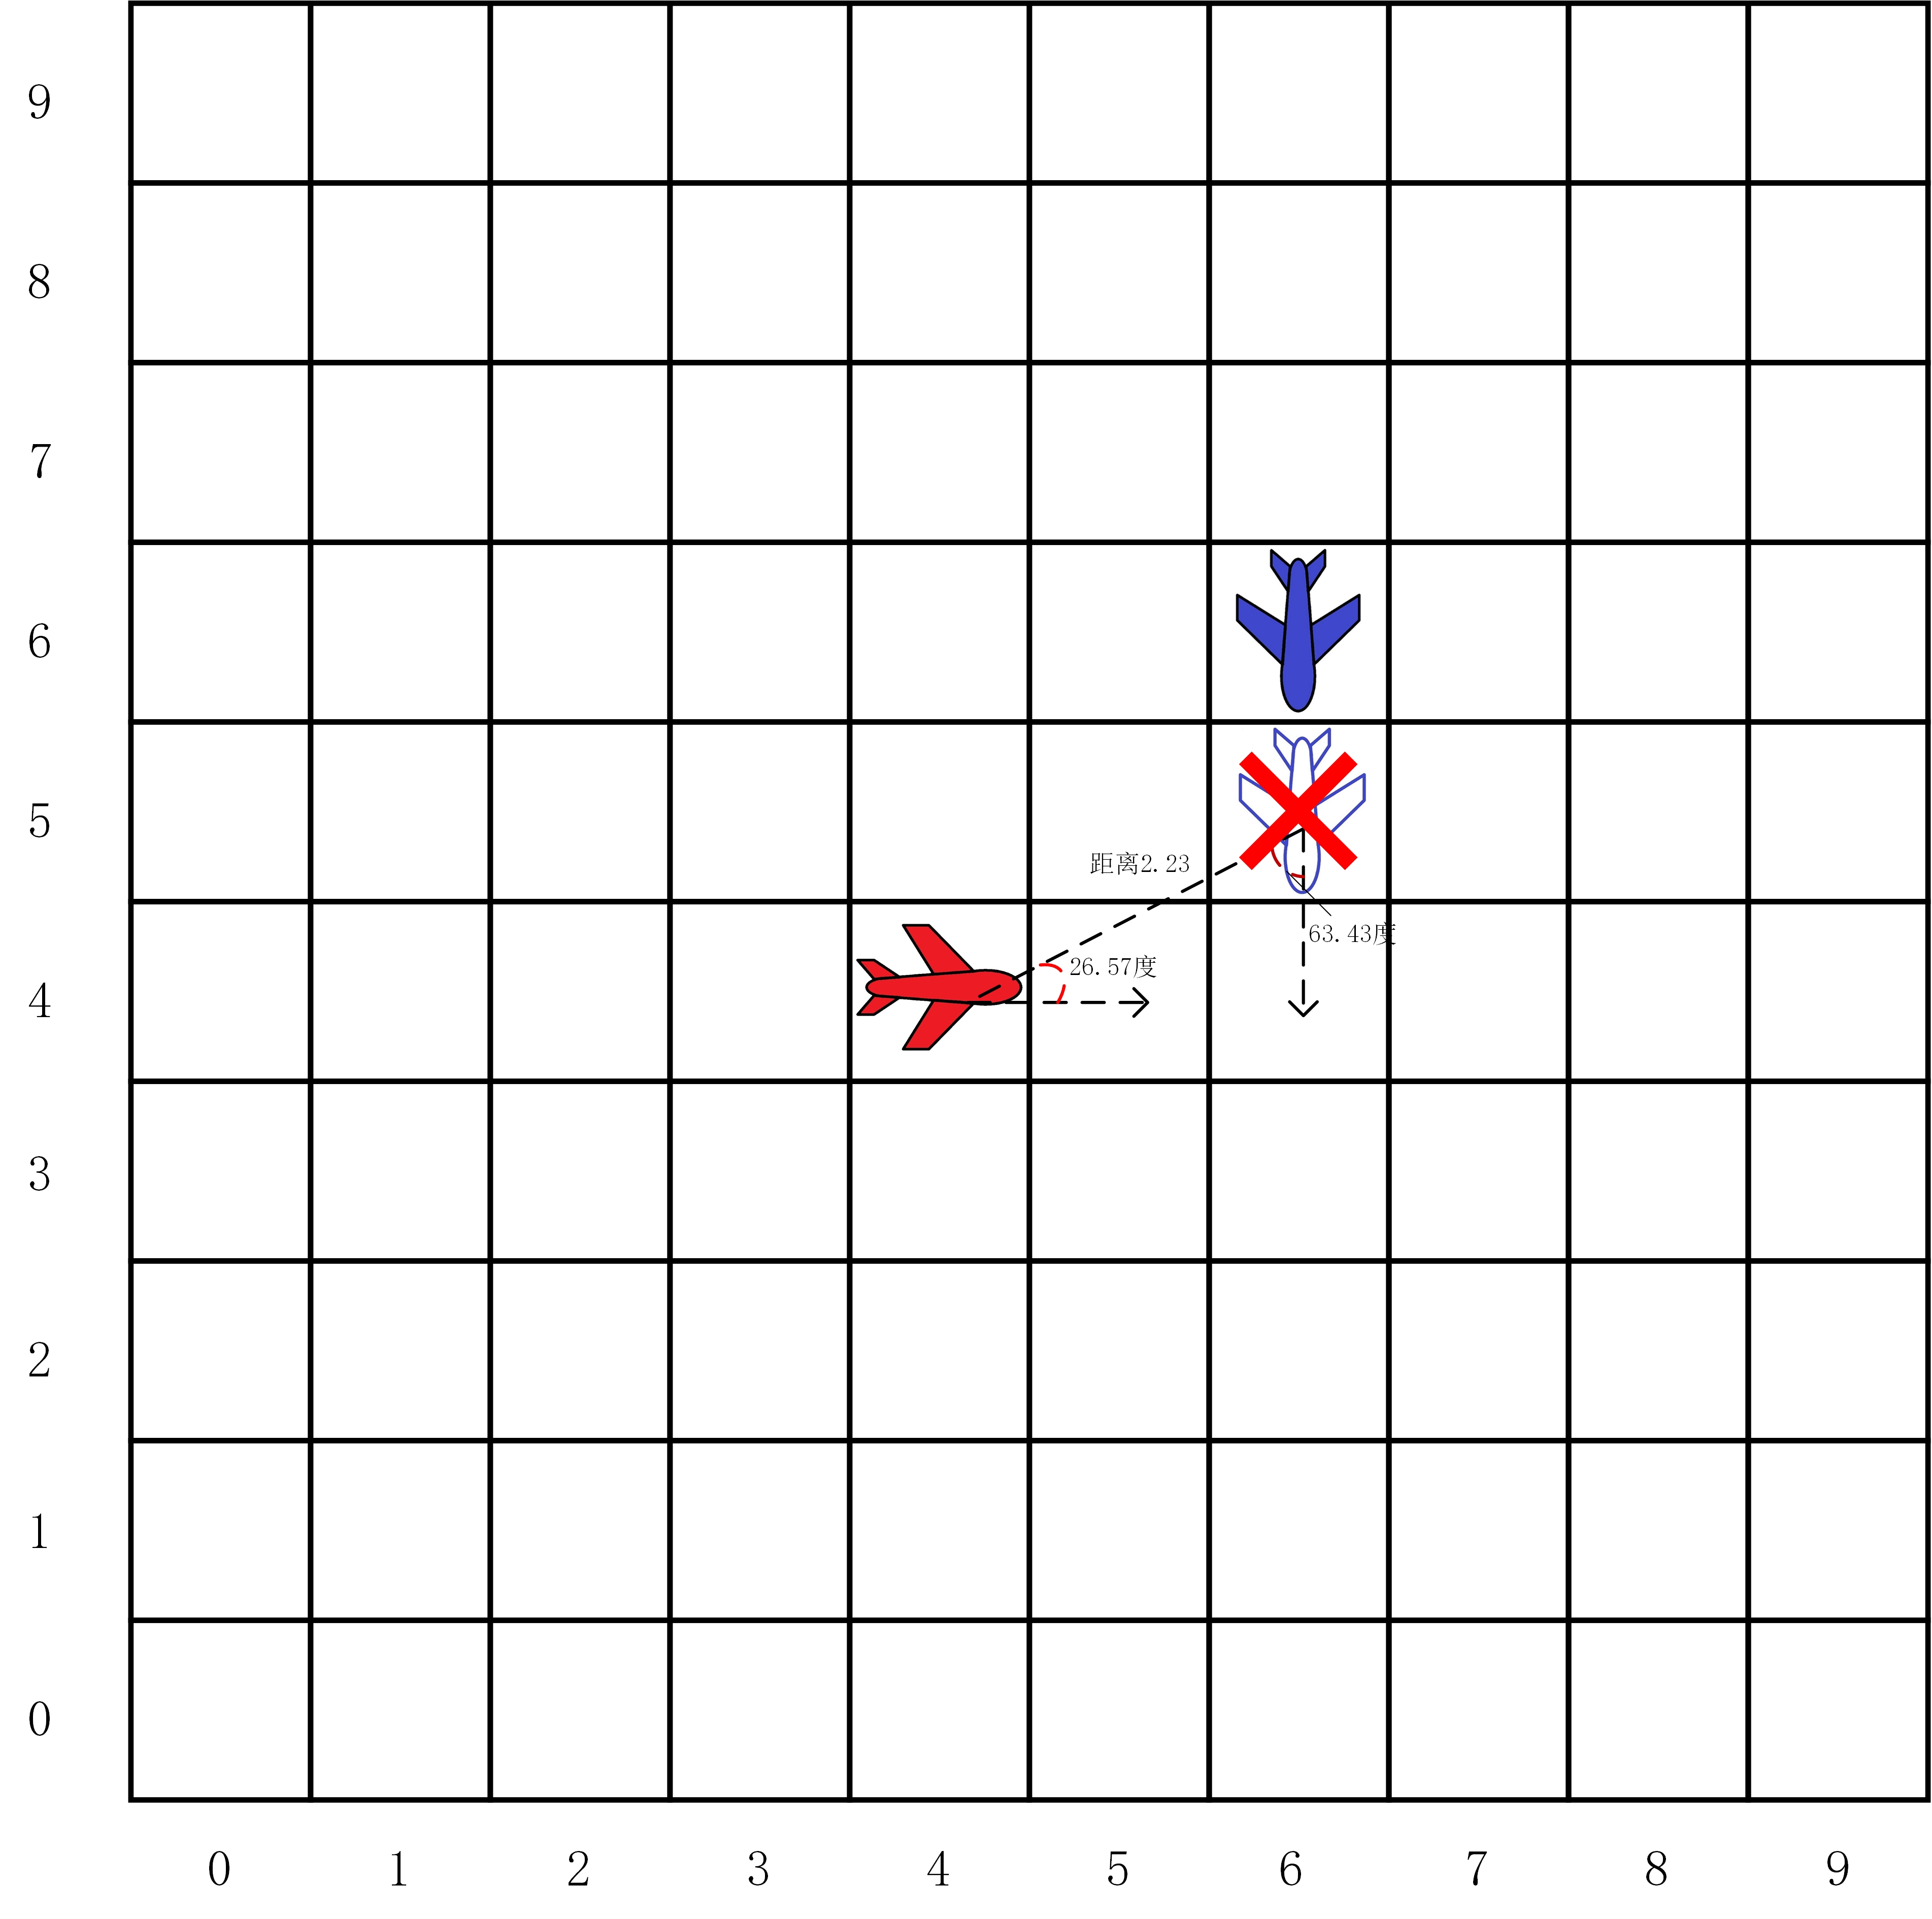
\includegraphics[width=0.45\hsize,height=0.45\hsize]{example/feijiyiduiyi8.jpg}}
	\newline
	\centering
	\subcaptionbox{向左双方状态\label{fig2:yiduiyi7-10:c}}
	{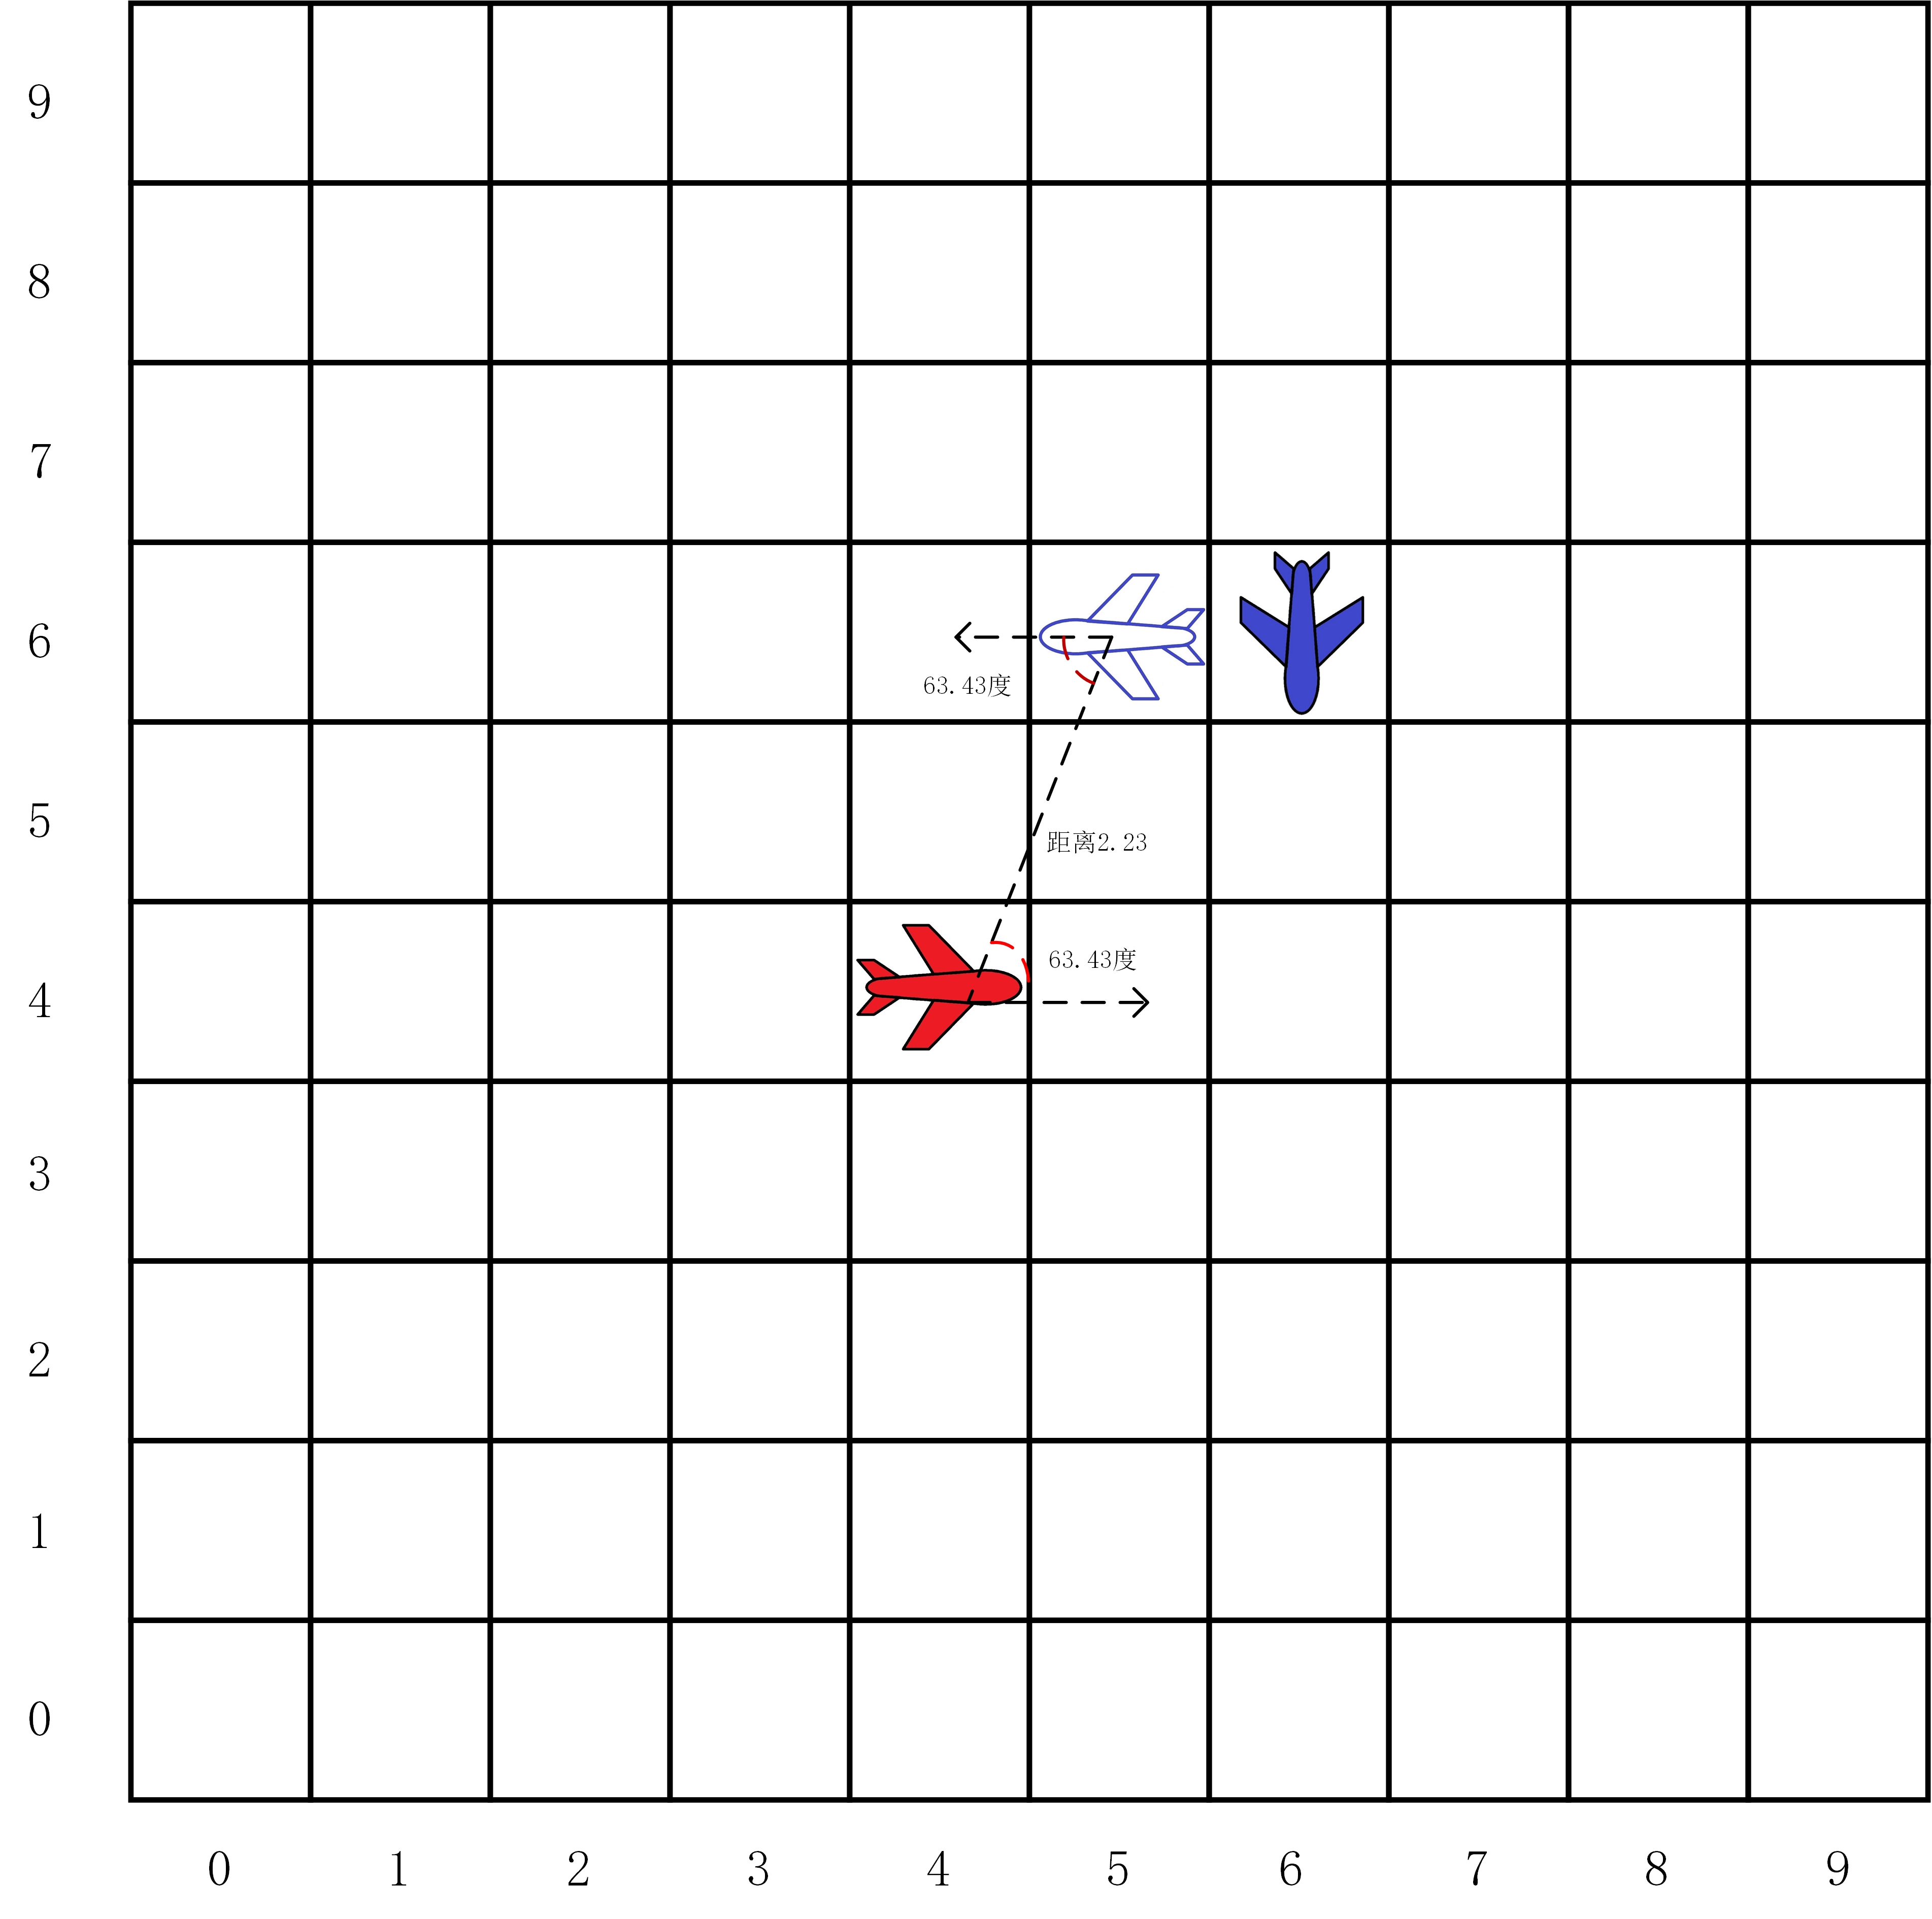
\includegraphics[width=0.45\hsize,height=0.45\hsize]{example/feijiyiduiyi9.jpg}}
	\hspace{0.5em}
	\subcaptionbox{向右双方状态\label{fig2:yiduiyi7-10:d}}
	{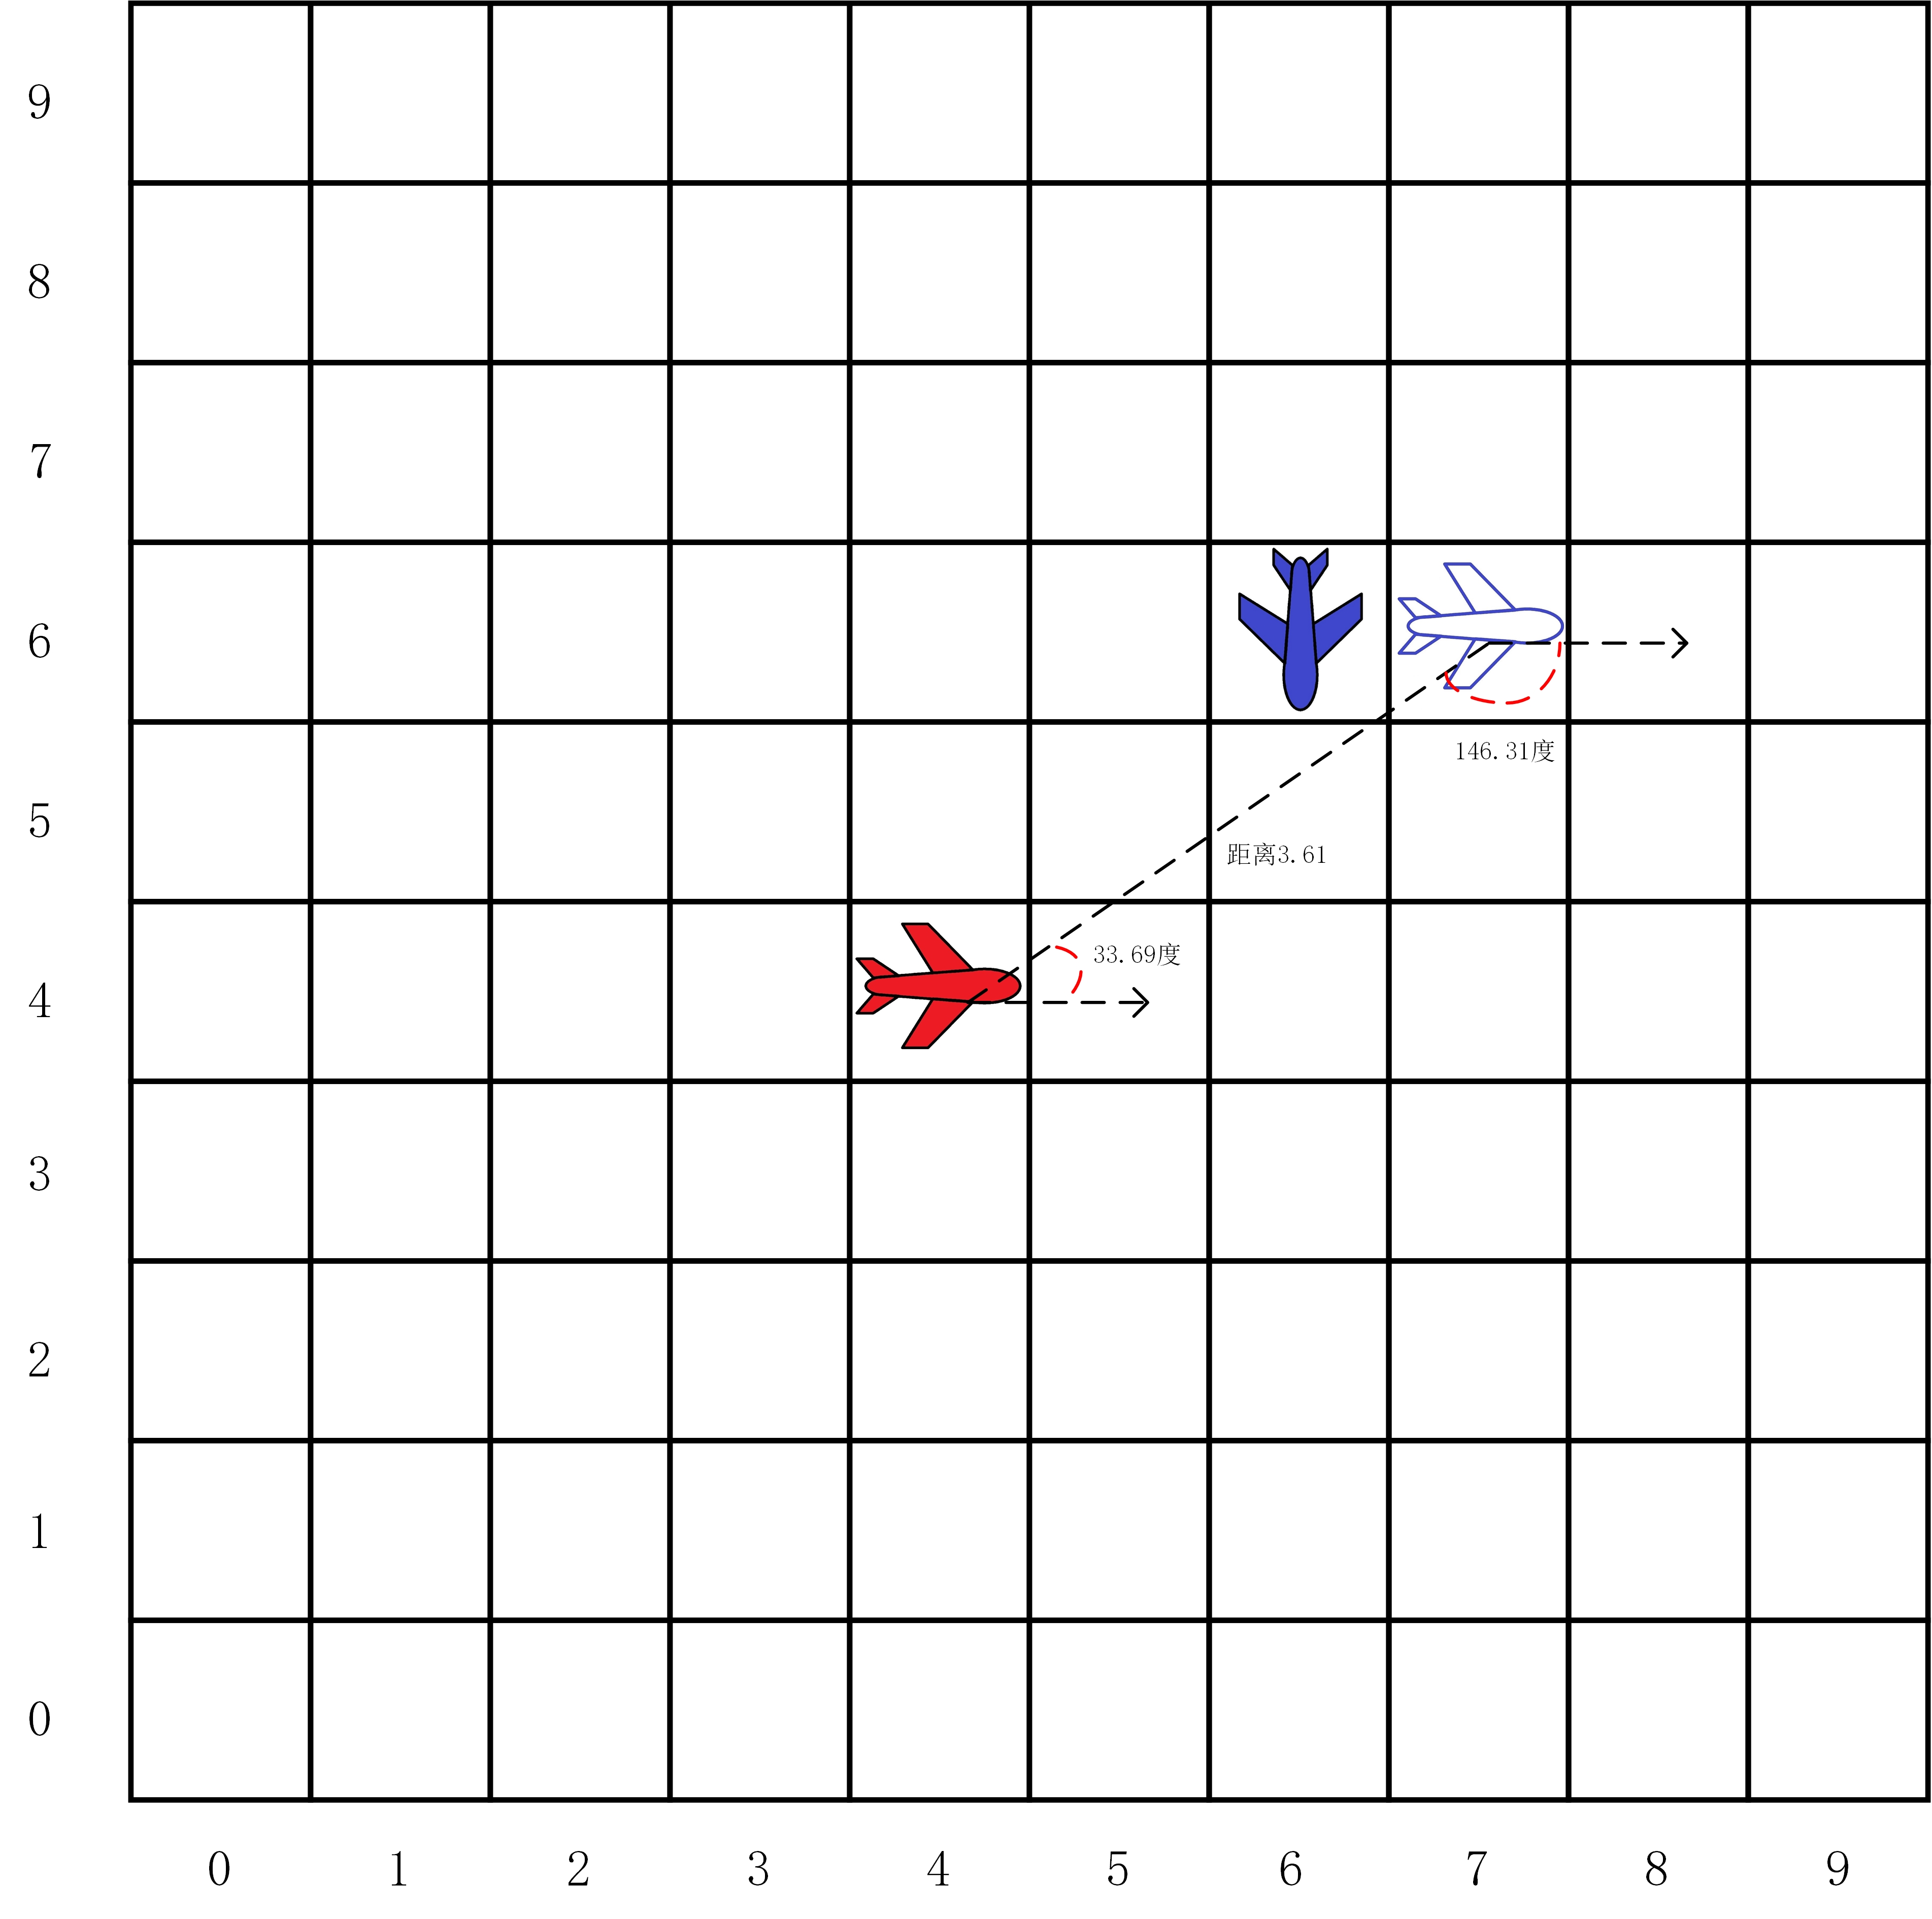
\includegraphics[width=0.45\hsize,height=0.45\hsize]{example/feijiyiduiyi10.jpg}}
	\bicaption[一对一人机对弈状态分析(1)]
	{一对一人机对弈状态分析(1)}
	{Analysis of one-on-one man-machine game status(1).}
	\label{fig2:yiduiyi7-10}
\end{figure}

可以看出当蓝方向下走时,会被红方击落,对模型搜索得到的概率为0.0375。而选择向左靠近红方时达不到最佳击落红方的位置,AI的策略是远离红方寻找下一个最佳攻击位置。在图\ref{fig2:yiduiyi3-6:c}状态时,对于蓝方执行四个动作进行分析,如图\ref{fig2:yiduiyi11-14}。当蓝方远离红方后获得了更小的攻击角。分析其可能的四个动作,当蓝方向下时会把红方击落,对照蒙特卡洛搜索得到的概率,向下的概率最大,为0.755。

\begin{figure}[htpb]
	\centering
	\subcaptionbox{向上双方状态\label{fig2:yiduiyi11-14:a}}
	{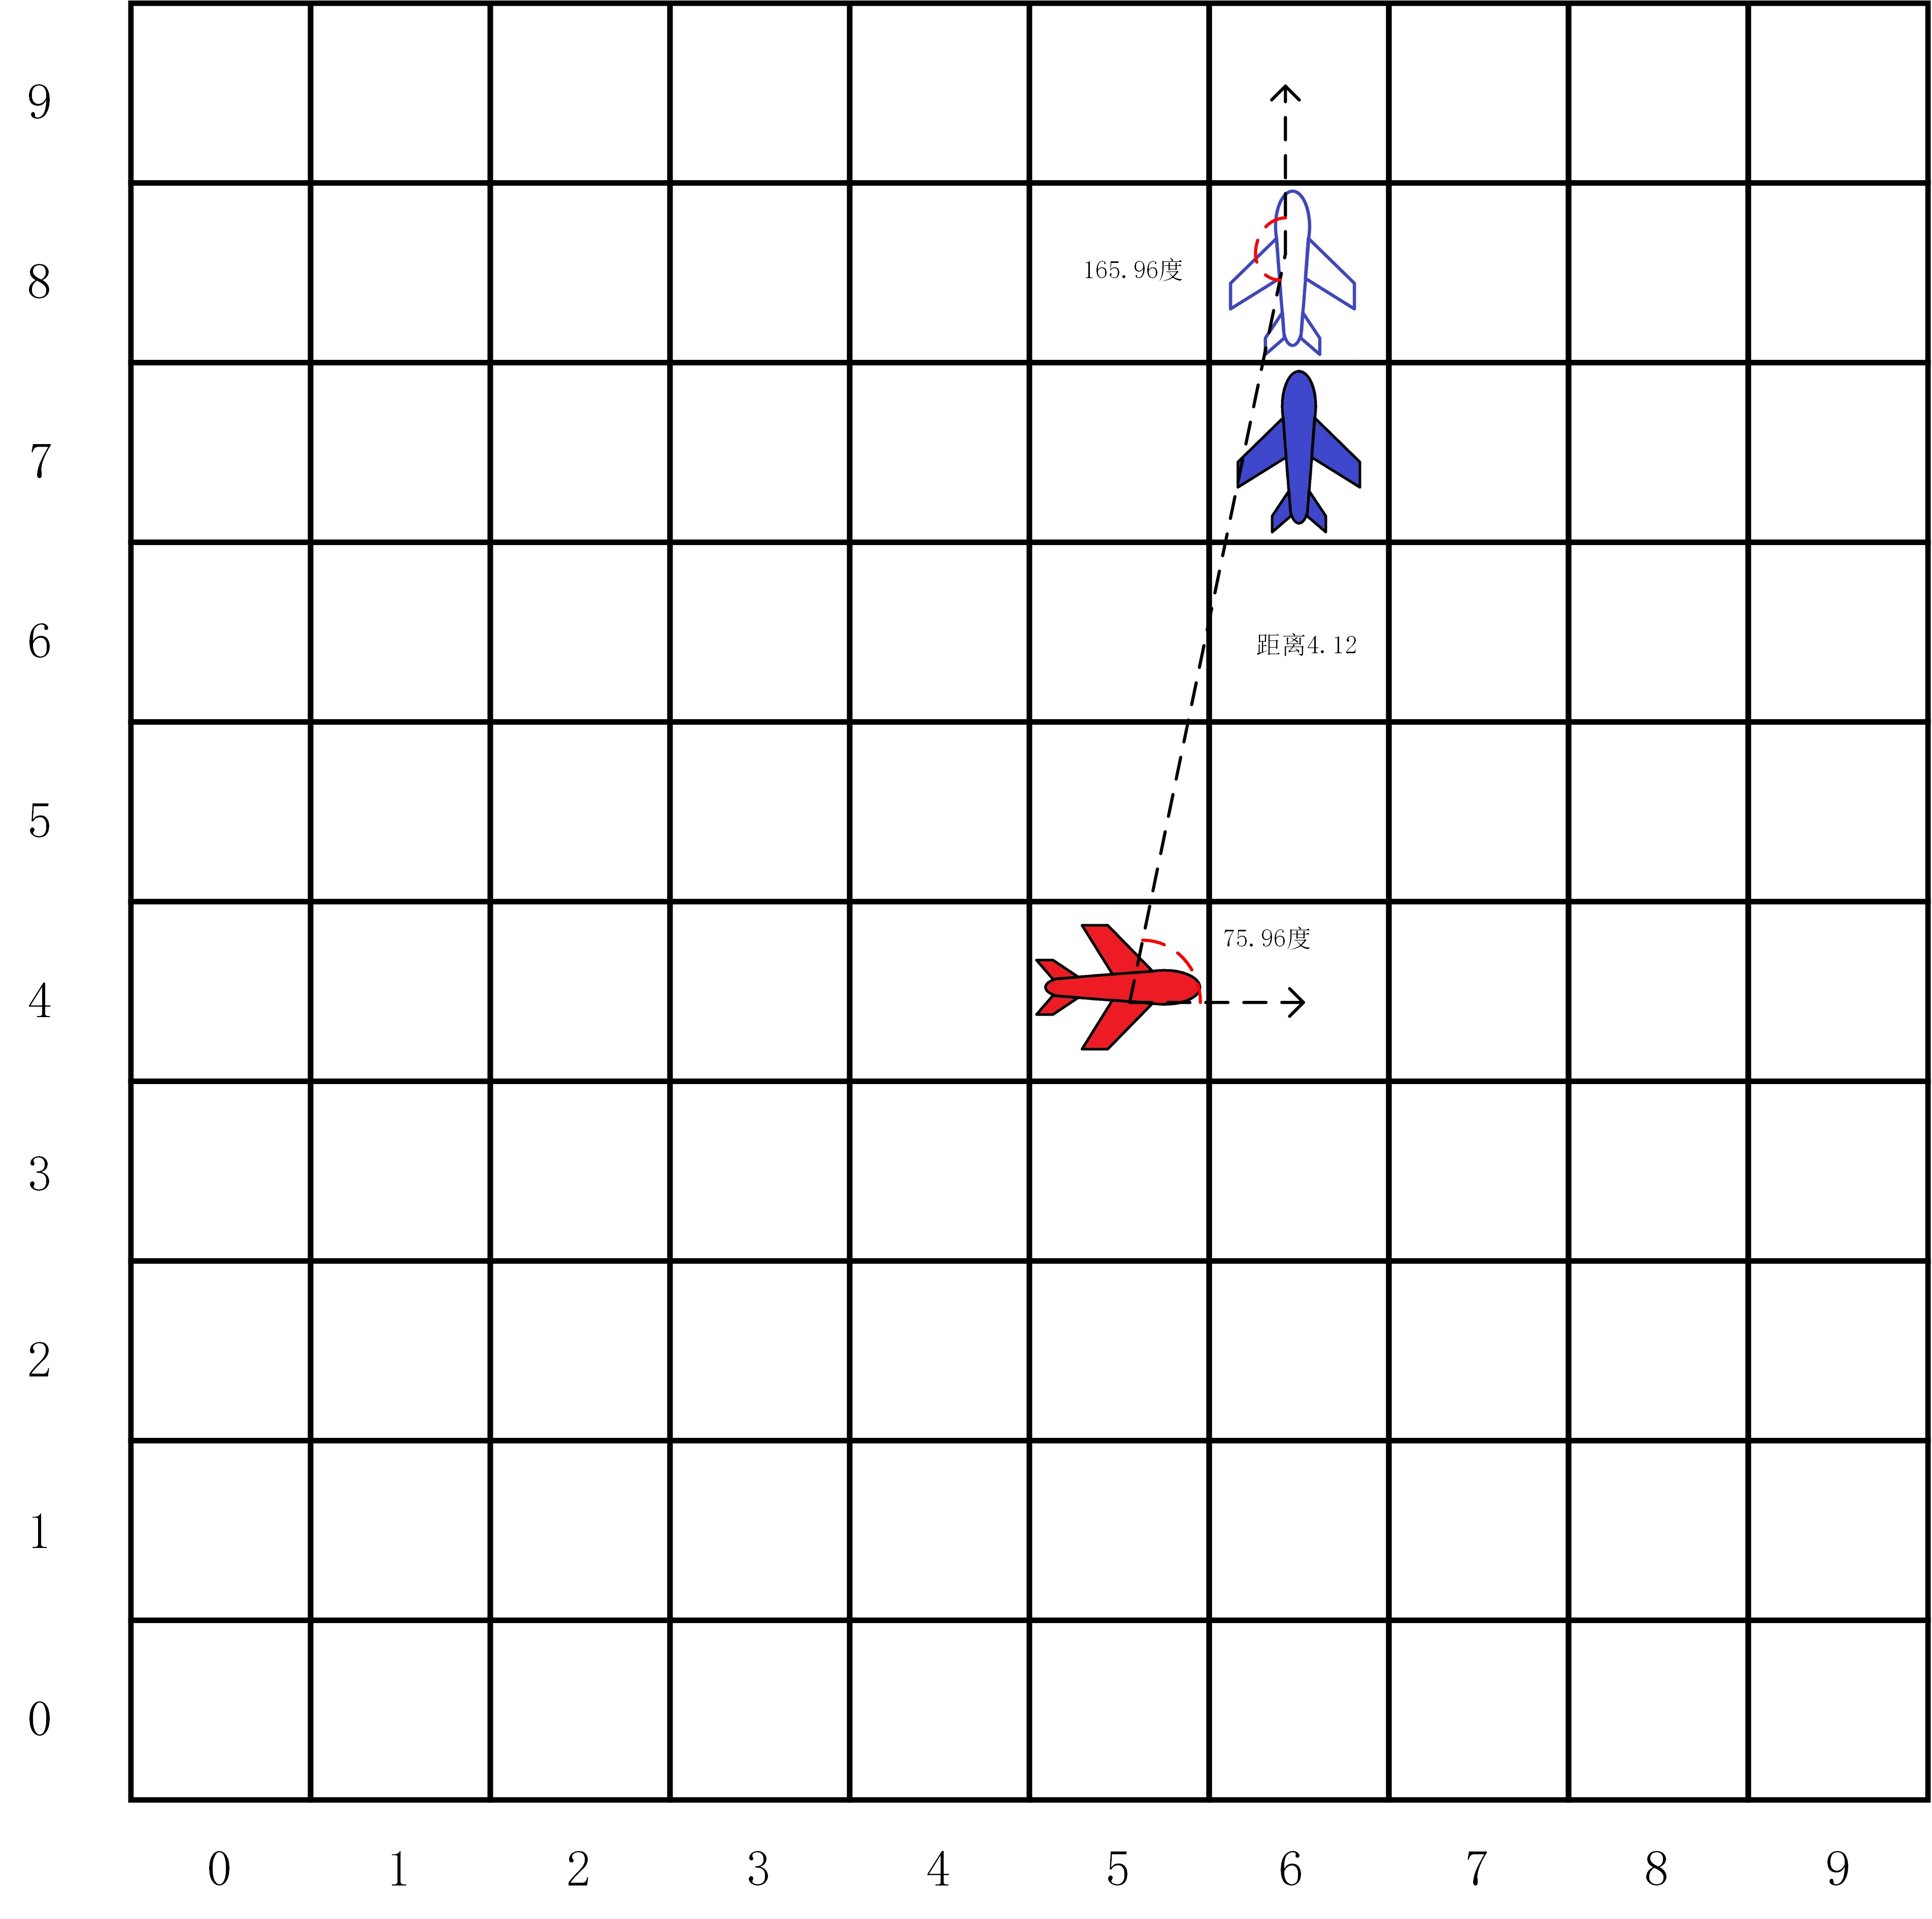
\includegraphics[width=0.45\hsize,height=0.45\hsize]{example/feijiyiduiyi11.jpg}}
	\hspace{0.5em}
	\subcaptionbox{向下双方状态\label{fig2:yiduiyi11-14:b}}
	{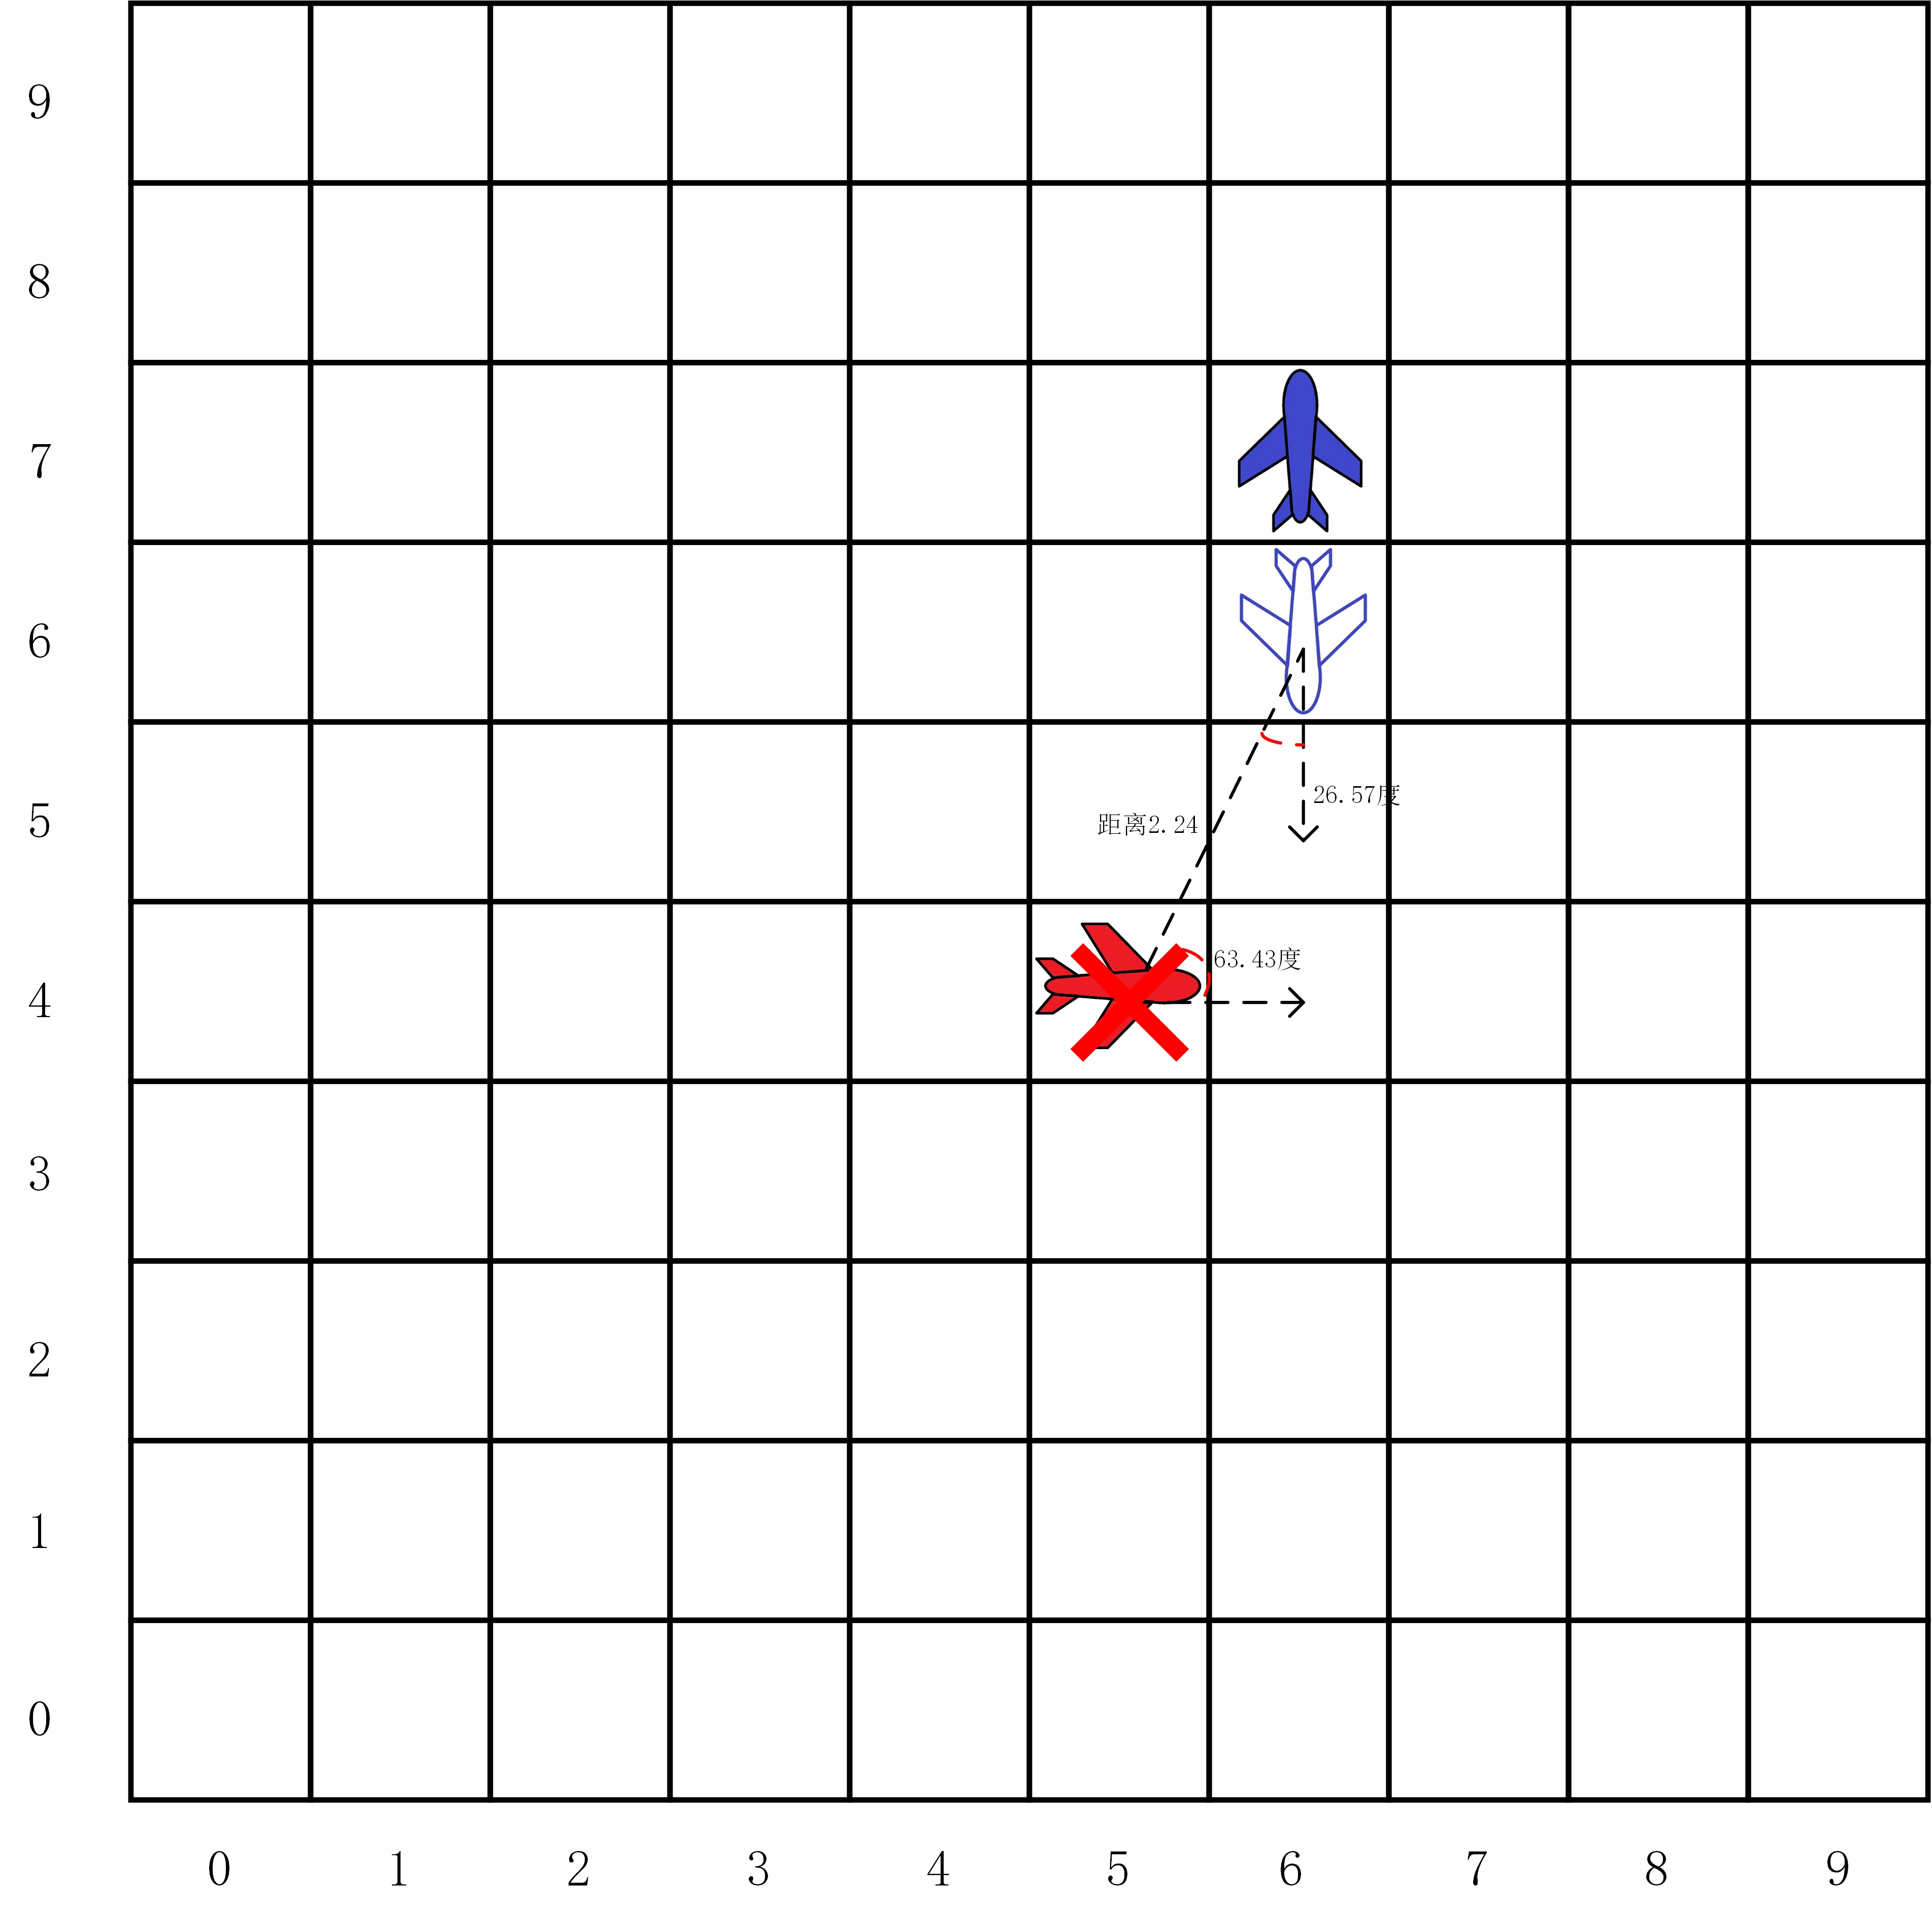
\includegraphics[width=0.45\hsize,height=0.45\hsize]{example/feijiyiduiyi12.jpg}}
	\newline
	\centering
	\subcaptionbox{向左双方状态\label{fig2:yiduiyi11-14:c}}
	{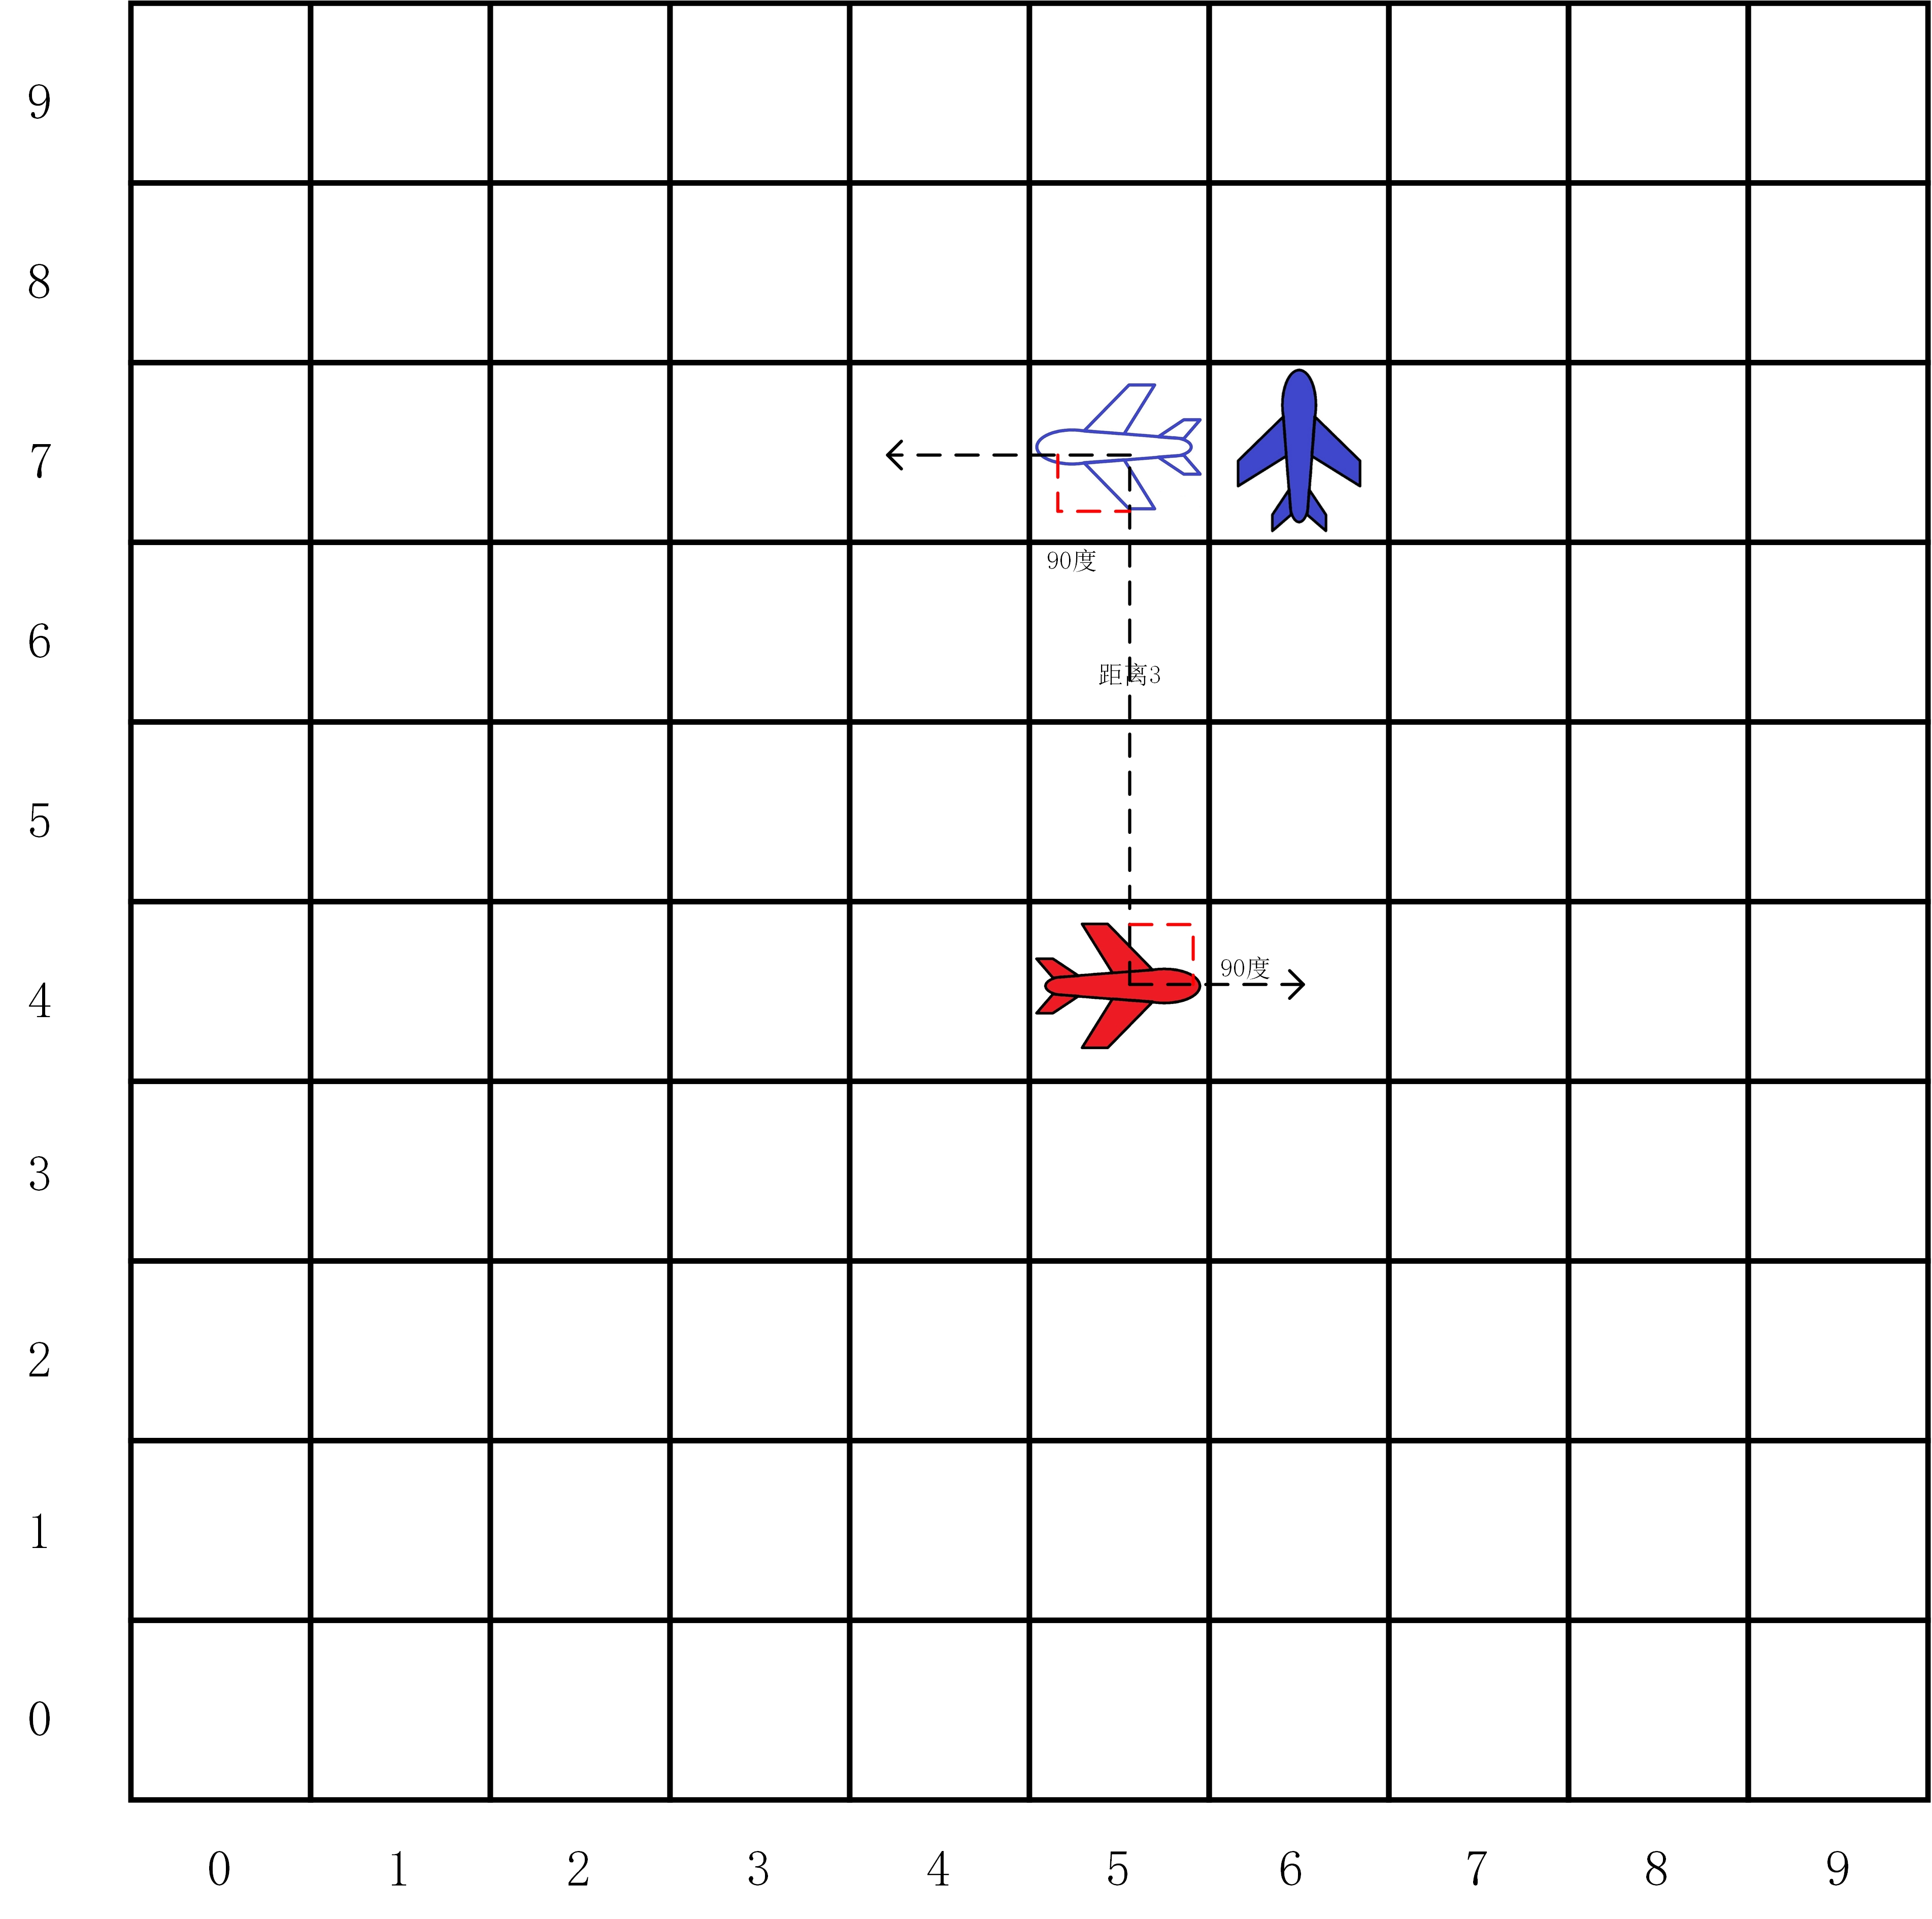
\includegraphics[width=0.45\hsize,height=0.45\hsize]{example/feijiyiduiyi13.jpg}}
	\hspace{0.5em}
	\subcaptionbox{向右双方状态\label{fig2:yiduiyi11-14:d}}
	{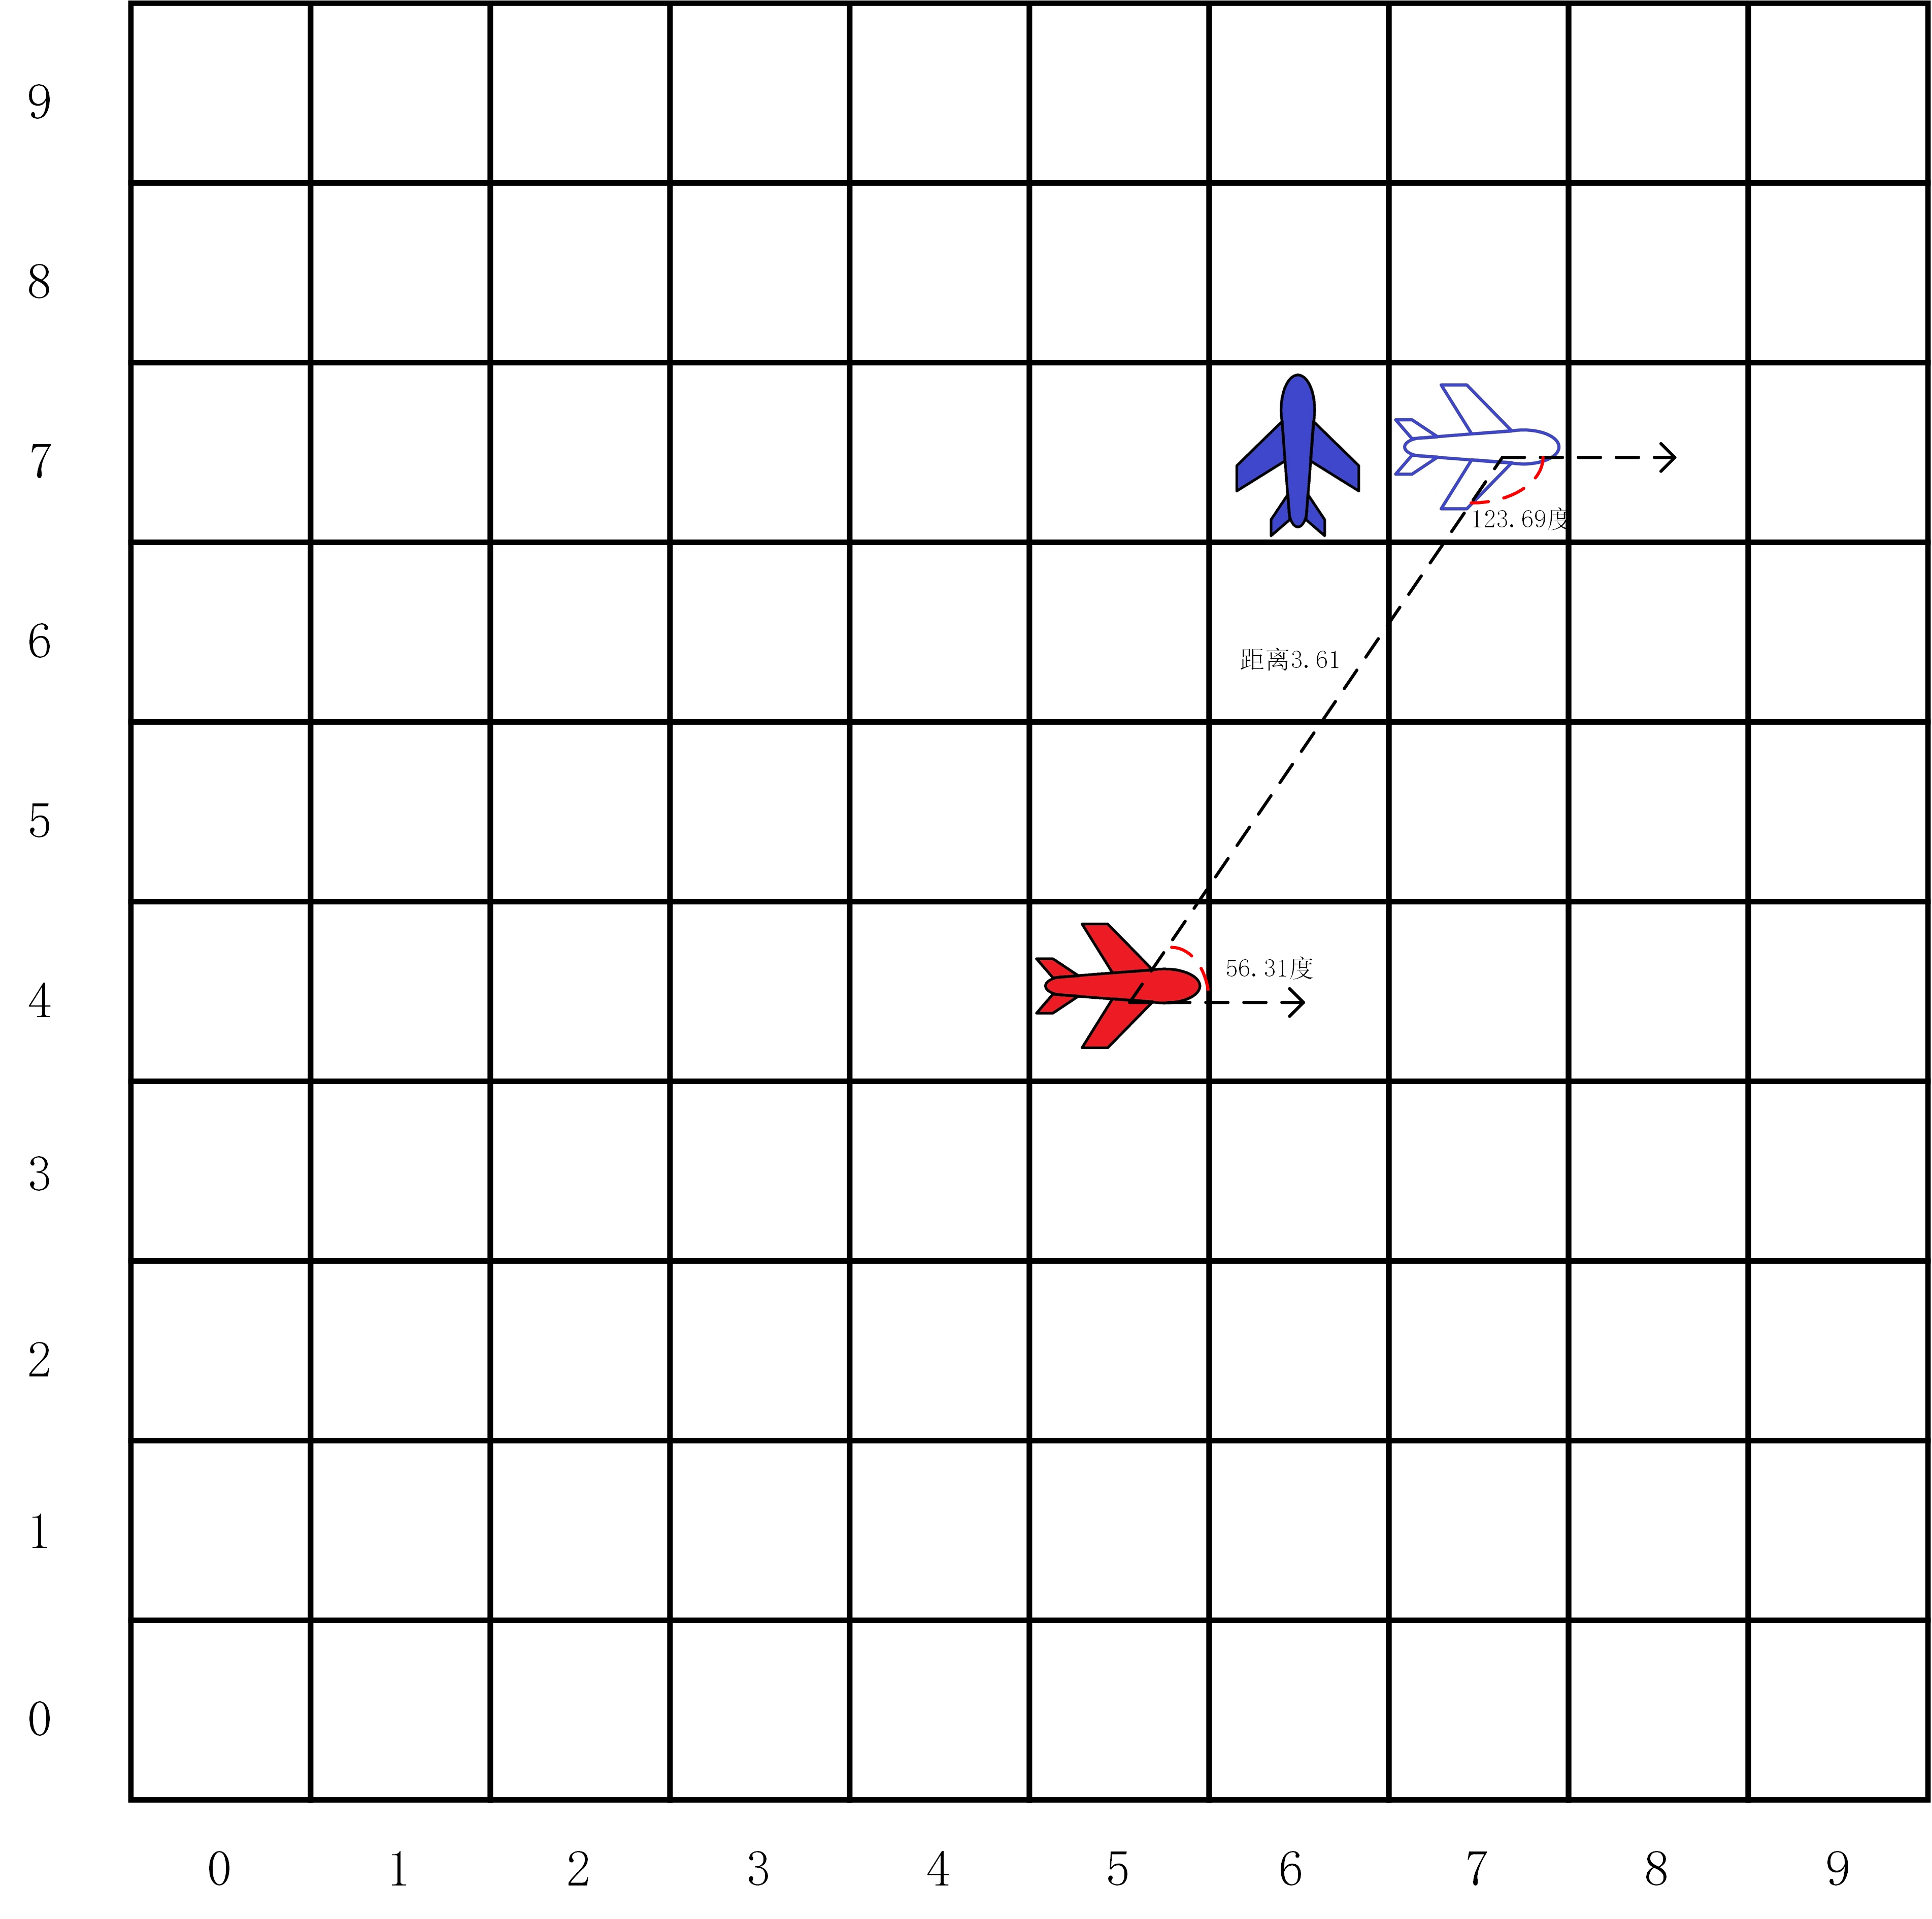
\includegraphics[width=0.45\hsize,height=0.45\hsize]{example/feijiyiduiyi14.jpg}}
	\bicaption
	{一对一人机对弈状态分析(2)}
	{Analysis of man-machine game status(2).}
	\label{fig2:yiduiyi11-14}
\end{figure}


本实验设计了一对一智能体对抗的场景,通过设置合理的参数,对训练出来的模型进行人机博弈实验,并详细跟踪了博弈关键步骤的模型输出结果,模型输出的策略和经过计算分析得到的策略一致。可以看出训练后的模型已经能够进行自主决策,并寻找合适的位置在最小的步数内攻击获胜。

\section{二对二智能体对抗}
上一节介绍的是一对一智能体之间的博弈问题,本节将进一步研究二对二智能体对抗问题。对于多个智能体之间既有合作又有对抗的情况,奖励的合理分配是至关重要的。在传统的经典算法中,奖励分配是人为设定规则进行奖励分配和战术调整。在本节我们用深度强化学习处理多个智能体之间的竞争与合作的关系。
\subsection{基于AC框架下的多智能体强化学习}
经典的多智能体算法都是基于Q值学习进行策略更新的。当其他智能体进行动作时,需要不断更新当前智能体的Q值函数表,同时奖励的分配也是需要加规则进行干预的。本节用AC框架进行多智能体强化学习的研究,奖励不需要人为分配,通过Critic函数告诉Actor当前动作的得分,对于一个有$N$个智能体的博弈环境,假设其策略梯度的参数为$\theta  = \{ {\theta _1},...{\theta _N}\} $,其策略的集合为$\pi  = \{ {\pi _1},...{\pi _N}\} $,对于第$i$个智能体,其期望收益的梯度$J({\theta _i}) = E[{R_i}]$如式\ref{eq:tidu}。
\begin{equation}
\label{eq:tidu}
{\nabla _{{\theta _i}}}J({\theta _i}) = {E_{s \sim {p^u},{a_i} \sim {\pi _i}}}[{\nabla _{{\theta _i}}}\log {\pi _i}({a_i}|{o_i}){Q_i}^\pi ({a_i},...{a_N})]
\end{equation}
${\nabla _{{\theta _i}}}J({\theta _i}) = {E_{s \sim {p^u},{a_i} \sim {\pi _i}}}[{\nabla _{{\theta _i}}}\log {\pi _i}({a_i}|{o_i}){Q_i}^\pi ({a_i},...{a_N})]$
其中${Q_i}^\pi ({a_i},...{a_N})$是将所有智能体的动作信息作为输入,对当前智能体的期望收益作为输出的打分函数。对于每一个智能体都有自己的奖励函数结构,因此这个打分函数可以学习到合作和竞争混合的结构。经验池中存储了每一个智能体的观测状态,动作信息和奖励$(x,{a_1},...{a_N},{r_1},...,{r_N})$,
对于每一个智能体,其策略梯度函数的更新方式如式\ref{gengxin}。
\begin{equation}
\label{gengxin}
L({\theta _i}) = {E_{x,a,r,x'}}[{({Q_i}^u(x,{a_1},...,{a_N}) - y)^2}]
\end{equation}

其中$y = {r_i} + \gamma {Q_i}^{u'}(x',{a_1}^\prime ,...,{a'_N}){|_{{{a'}_j} = {{u'}_j}({o_j})}}$
这里$u' = \{ {u_{{{\theta '}_1}}},...,{u_{{{\theta '}_N}}}\} $是当其他智能体进行动作后新的策略。

当利用AC模型进行建模时,对于一对一智能体的网络结构,策略网络和价值网络是特征输入平面是相同的,对于多对多智能体作战而言,对于每个智能体不仅要考虑到敌方智能体的位置,还要考虑我方其他智能体的状态。所以在设计输入特征时候需要考虑其他智能体的状态和动作信息。在蒙特卡洛搜索树中每个智能体进行动作后都应相应的扩展一层叶子节点,同时要考虑树的叶子节点回传的过程。
\subsection{问题描述}
本节在上一节的基础上,由一对一智能体之间的相互博弈拓展到二对二智能体的相互博弈。击落敌方一架飞机的规则和上一节相同,即距离小于4个格子长度,追击角小于$30^\circ$,敌方飞机逃逸角大于$30^\circ$。这里红方蓝方各有两架飞机,给两方飞机一个初始速度和位置,作战规则如下:四架飞机轮流进行移动,行动的范围是上下左右,当下一动作超出作战范围或撞到本方飞机时,认为该动作是非法的。智能体动作的顺序为红一,蓝一,红二,蓝二,依次循环直到有一方获胜。游戏结束的规则为当有任意一方有至少一架飞机被击落,该方判为输家。因此整个游戏的流程如算法\ref{erduierliucheng}所示。
\begin{algorithm}[htbp]
	\caption{飞机二对二作战流程}% Ëã·¨±êÌâ
	\label{erduierliucheng}
	\begin{algorithmic}[1]%Ò»ÐÐÒ»¸ö±êÐкÅ
		\For{每架飞机移动的次数不超过移动步数上限 }
		\State 红一根据强化学习策略从合法动作中选择一个进行动作
		\State 判断红一和蓝方两架飞机的状态关系
		\If {任意一架飞机被击落}
		\State 游戏结束,跳出循环,返回结果
		\EndIf
		\State 蓝一根据强化学习策略从合法动作中选择一个进行动作
		\State 判断蓝一和红方两架飞机的状态关系
		\If {任意一架飞机被击落}
		\State 游戏结束,跳出循环,返回结果
		\EndIf
		\State 红二根据强化学习策略从合法动作中选择一个进行动作
		\State 判断红二和蓝方两架飞机的状态关系
		\If {任意一架飞机被击落}
		\State 游戏结束,跳出循环,返回结果
		\EndIf
		\State 蓝二根据强化学习策略从合法动作中选择一个进行动作
		\State 判断蓝二和红方两架飞机的状态关系
		\If {任意一架飞机被击落}
		\State 游戏结束,跳出循环,返回结果
		\EndIf
		\EndFor
	\end{algorithmic}
\end{algorithm}

\subsection{场景建模}

在二对二场景中,相当于每个智能体不仅需要感知当前状态,还需要感知本方智能体和敌方智能体所有的动作信息。智能体的动作可以通过上一步的位置和当先位置得到,所以在本实验中状态设置为$10 \times 10 \times 9$。其中,$10 \times 10$代表棋盘大小,第一层是红一当前位置,第二层为红一上一步位置,第三层第四层依次表示红二当前位置和上一步位置,第五,六层为蓝一信息,第七,八层为蓝二信息,第九层用来标识当前玩家,可选数值为0,1,2,3。所有飞机的位置信息,动作信息都可以从状态空间中反解出来。由于设计的状态包含了当前环境状态和其他智能体的动作信息,在利用深度学习网络拟合值函数和策略函数时,特征提取部分的网络结构可以共享,深度学习网络结构如图\ref{fig:wangluojiegoutu}所示。网络分为共用的特征提取部分,策略网络后面用softmax函数进行4分类,价值网络后面用tanh函数进行回归。数据的标签通过蒙特卡洛搜索树得到。

\begin{figure}[htpb]
	\centering
	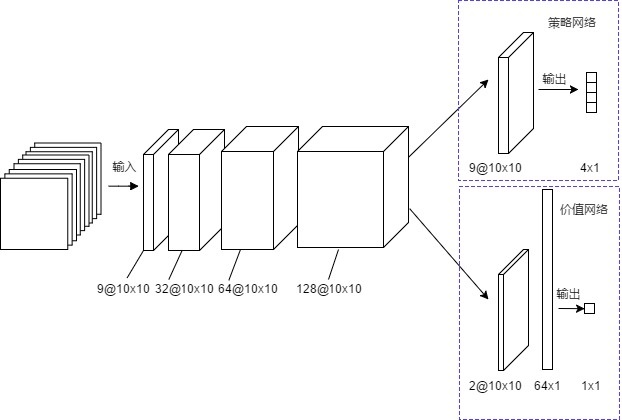
\includegraphics[width=10cm]{example/wangluojiegoutu.jpg}
	\bicaption[二对二深度学习网络结构图]
	{二对二深度学习网络结构图}
	{Neural network training pipeline}
	\label{fig:wangluojiegoutu}
\end{figure}

二对二强化学习博弈算法流程如算法\ref{duoduiduosuanfa}所示。在监测网络结构是否是最优的时候,保存当前最新模型和历史最优模型进行相互博弈,当获胜率大于一定阈值时,进行网络参数的更新,否则最优模型不变。
\begin{algorithm}[htbp]
	\caption{二对二强化学习博弈算法}% Ëã·¨±êÌâ
	\label{duoduiduosuanfa}
	\begin{algorithmic}[1]%Ò»ÐÐÒ»¸ö±êÐкÅ
		\Require
		包含当前位置和历史走过位置的状态信息,游戏动作规则,游戏奖励规则。随机初始化神经网络的参数$\theta_0$
		\Ensure 
		动作策略$p$,状态价值$v$
		\For{每一次迭代$iteration=1$ to $T$ }
		 \If{达到下列之一终止条件:
		 \begin{enumerate}
		     	 \item 所有智能体都没有可选动作
		     	 \item 达到了游戏最大的行动数还没分出胜负
	     \end{enumerate}}
		\State 跳出当前循环
		\Else
		\State 继续进行本次循环
		\EndIf
		\State 初始化状态$S_0$
		\For {对于在$t$时刻的动作}
		\State 利用$MCTS$算法进行搜索
		\While{$MCTS$搜索次数小于$n_playout$}
		\State 进行树节点的选择:每次模拟通过选择最大上限置信度$Q(s,a)+U(s,a)$进行树的遍历。这里${\rm{U}}(s,a) \propto P(s,a)/(1 + N(s,a))$
		\State 叶节点的扩展和状态值评估:
		利用神经网络计算结果进行叶节点展开和对应状态值的评估。$(P(s, \cdot ),V(s)) = {f_{{\theta _i}}}(s)$,$p$值的向量存储在从$s$输出的边中。
		\State 回溯:
		当进行树的模拟遍历时,被访问的边会进行相应的节点访问次数更新,$Q(s,a) = 1/N(s,a)\sum\nolimits_{s'|s,a \to s'} {V(s')} $,这里${s'|s,a \to s'}$代表在状态$s$采取动作$a$后到达状态$s'$。
		\EndWhile
		\State 动作选择:
		\\当搜索结束后,根据搜索的结果根据式\ref{eq:gailu}结合温度参数统计每个动作被访问的概率。根据得到的结果选择一个动作进行到下一状态$s_t+1$的转移。
		\EndFor
		  \algstore{MergeSort}
		\end{algorithmic}
		\end{algorithm}

		\begin{algorithm}[htbp]
		\begin{algorithmic}[1]
		\algrestore{MergeSort}
		\State 记录当前幕中经过的所有的状态和最后游戏的结果${r_T} \in \{  - 1, + 1\} $
		\For{在得到最后的获胜结果后,对于之前走过的每一步}
		\State 从当前玩家角度更新最后游戏的得分${z_t} \leftarrow  \pm {r_T}$,结合之前保存的每一步状态,存储数据的格式为$s_t,\pi_t,z_t$
		\EndFor
		\State 对于最新模型self-play产生的数据进行随机采样。
		\State 通过以下损失函数:
		\begin{equation}
		l = {(z - v)^2} - {\pi ^T}\log p + c||{\theta _i}{\rm{|}}{{\rm{|}}^{\rm{2}}}
		\end{equation}
		最大化策略网络输出的概率分布和蒙特卡洛搜索树得到的概率之间的相似度,同时最小化价值函数的预测得分和$self-play$得到的最后结果之间的误差。
		调整输入给蒙特卡洛树的神经网络参数$(p,v) = {f_{{\theta _i}}}(s)$。
		\If {$iteration\%checkpoint==0$}
		\State 利用最新数据训练出来的模型(参数为$\theta '$)和之前最好的模型(参数为$\theta$)进行对弈
		\If {获胜率大于0.8}
		 \State 进行网络参数更新${\theta _{i + 1}} = \theta '$,用于下一次$self-play$数据生成中的先验概率。
		\Else
		 \State 不进行网络参数更新,${\theta _{{\rm{i + 1}}}}{\rm{ = }}\theta $
		\EndIf
		\EndIf
		\EndFor
	\end{algorithmic}
\end{algorithm}

算法描述可以看出,MCTS在深度学习输出的先验概率${f_{{\theta _{i - 1}}}}$基础上搜索策略${\pi _t} = {\alpha _{{\theta _{i - 1}}}}({s_t})$。树节点的连边建立了一系列状态动作对$(s,a)$,记录了先验概率$P(s,a)$,节点访问次数$N(s,a)$和状态动作值$Q(s,a)$。self-play的过程产生了策略迭代网络的带标签的数据,在每一次自我博弈中,选择获胜玩家的数据进行一个正样本。训练深度学习网络权重${\theta _i}$,价值网络损失函数为回归常用的均方误差${(z - v)^2}$,策略网络为交叉熵$ - {\pi ^T}\log p$。这里同时训练两个网络所以将两项目标函数进行加和,利用梯度下降法进行网络参数的更新。

\subsection{二对二实验结果及分析}
本节将就二对二飞机作战训练曲线和训练模型的人机对弈结果进行分析,同时对比了加入人类先验规则的模型。在二对二实验中,参数设置如表\ref{2dui2canshu}。

\begin{table}[htpb]
	\centering
	\bicaption[二对二实验参数信息]
	{二对二实验参数信息}
	{4 agents experiment parameter setting.}
	\label{2dui2canshu}
	\begin{tabular}{ll} \toprule
		参数名称   & 参数值  \\  \midrule
		棋盘大小 & 10*10 \\ 
		学习率调整参数$\lambda$ & 1.5 \\  
		温度探索参数$\tau$& 1.0 \\ 
		每次落子蒙特卡洛搜索次数 & 500 \\ 
		贪心策略$\epsilon$ & 0.75 \\  
		起始学习率$r$ & 2e-3\\
		噪声系数$\varepsilon$ &0.25\\
		\bottomrule
	\end{tabular}
\end{table}

红蓝两方的初始位置和速度信息如图\ref{fig:duoduiduo1-2:a}所示,红一初始位置为$(1,2)$,红二初始位置为$(2,2)$,初速度都为向上,蓝一初始位置为$(7,7)$,蓝二初始位置为$(8,7)$,初速度都为向下。飞机的朝向为飞机的速度方向。
奖励设置为当双方各走完200步没有分出胜负,判为平局,四架飞机各奖励0,当一方至少有一架飞机被击灭,获胜方两架飞机奖励为1,失败方两架飞机奖励为-1。为了加快收敛速度,人为定义规则,当双方距离小于7时,只能向相互靠近的方向移动,对比加入规则前后得到的交叉熵和损失函数曲线如图\ref{fig1:guize}。
\begin{figure}[hbpt]
	\centering
	\subcaptionbox{规则对交叉熵的影响\label{fig1:guize:a}}
	{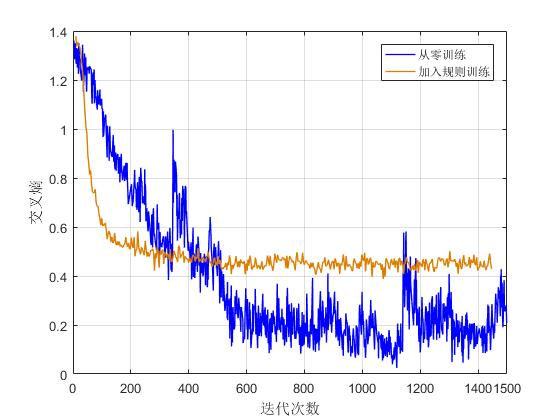
\includegraphics[width=0.45\hsize,height=0.45\hsize]{example/duoduiduoentropy.jpg}}
	\hspace{0.5em}
	\subcaptionbox{规则对损失函数的影响\label{fig1:guize:b}}
	{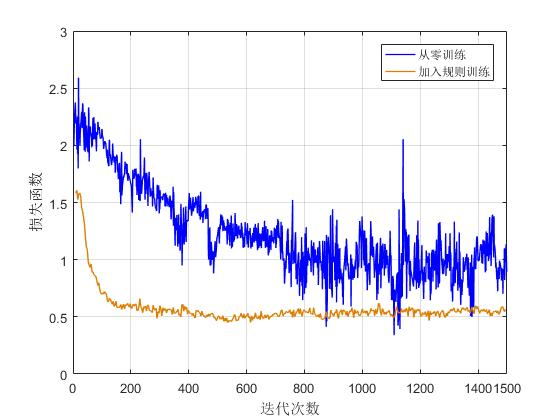
\includegraphics[width=0.45\hsize,height=0.45\hsize]{example/duoduiduoloss.jpg}}
	\bicaption[是否引入先验规则效果对比]
	{是否引入先验规则效果对比}
	{Comparison of whether introduce prior rule.}
	\label{fig1:guize}
\end{figure}

从图\ref{fig1:guize:a}可以看出在训练初期加入规则之前交叉熵下降相对缓慢,加入规则之后在训练初期交叉熵下降较快,但是在后期交叉熵稳定在0.45左右,而不加规则的模型交叉熵还在持续下降。从图\ref{fig1:guize:b}可以看出加入规则的模型损失函数相对容易学习,因为加入规则后人为干预了数据样本的多样性,所以网络更容易学习,但是同时失去了模型的泛化能力。

利用从零开始学迭代1500次后的最优模型和人进行对弈,人机对战结果展示如图\ref{fig:duoduiduo1-2:b}。在这里我方控制红方两架飞机,蓝方为训练AI的两架飞机,红方先行。红一可行动作为上,下,左,选择向上,到达位置$(1,4)$。计算红一和蓝一蓝二的位置信息,没有飞机被击落。轮到蓝一进行动作,蓝一可行的位置为上,下和左。经过500次蒙特卡洛搜索树搜索得到各个位置的概率信息如图\ref{fig:duoduiduo1-2:b}。模型在测试过程用贪心策略,选择概率最大的动作向左走,然后我方控制红二向右,接下来的对弈过程如图\ref{fig:duoduiduo3-6}所示。经过几回合的对战到达状态如图\ref{fig:duoduiduo3-6:d},可以看出这时对于蓝一的策略已经非常明确,模型以0.8375的概率向左移动。

\begin{figure}[!htbp]
	\centering
	\subcaptionbox{\label{fig:duoduiduo1-2:a}}
	{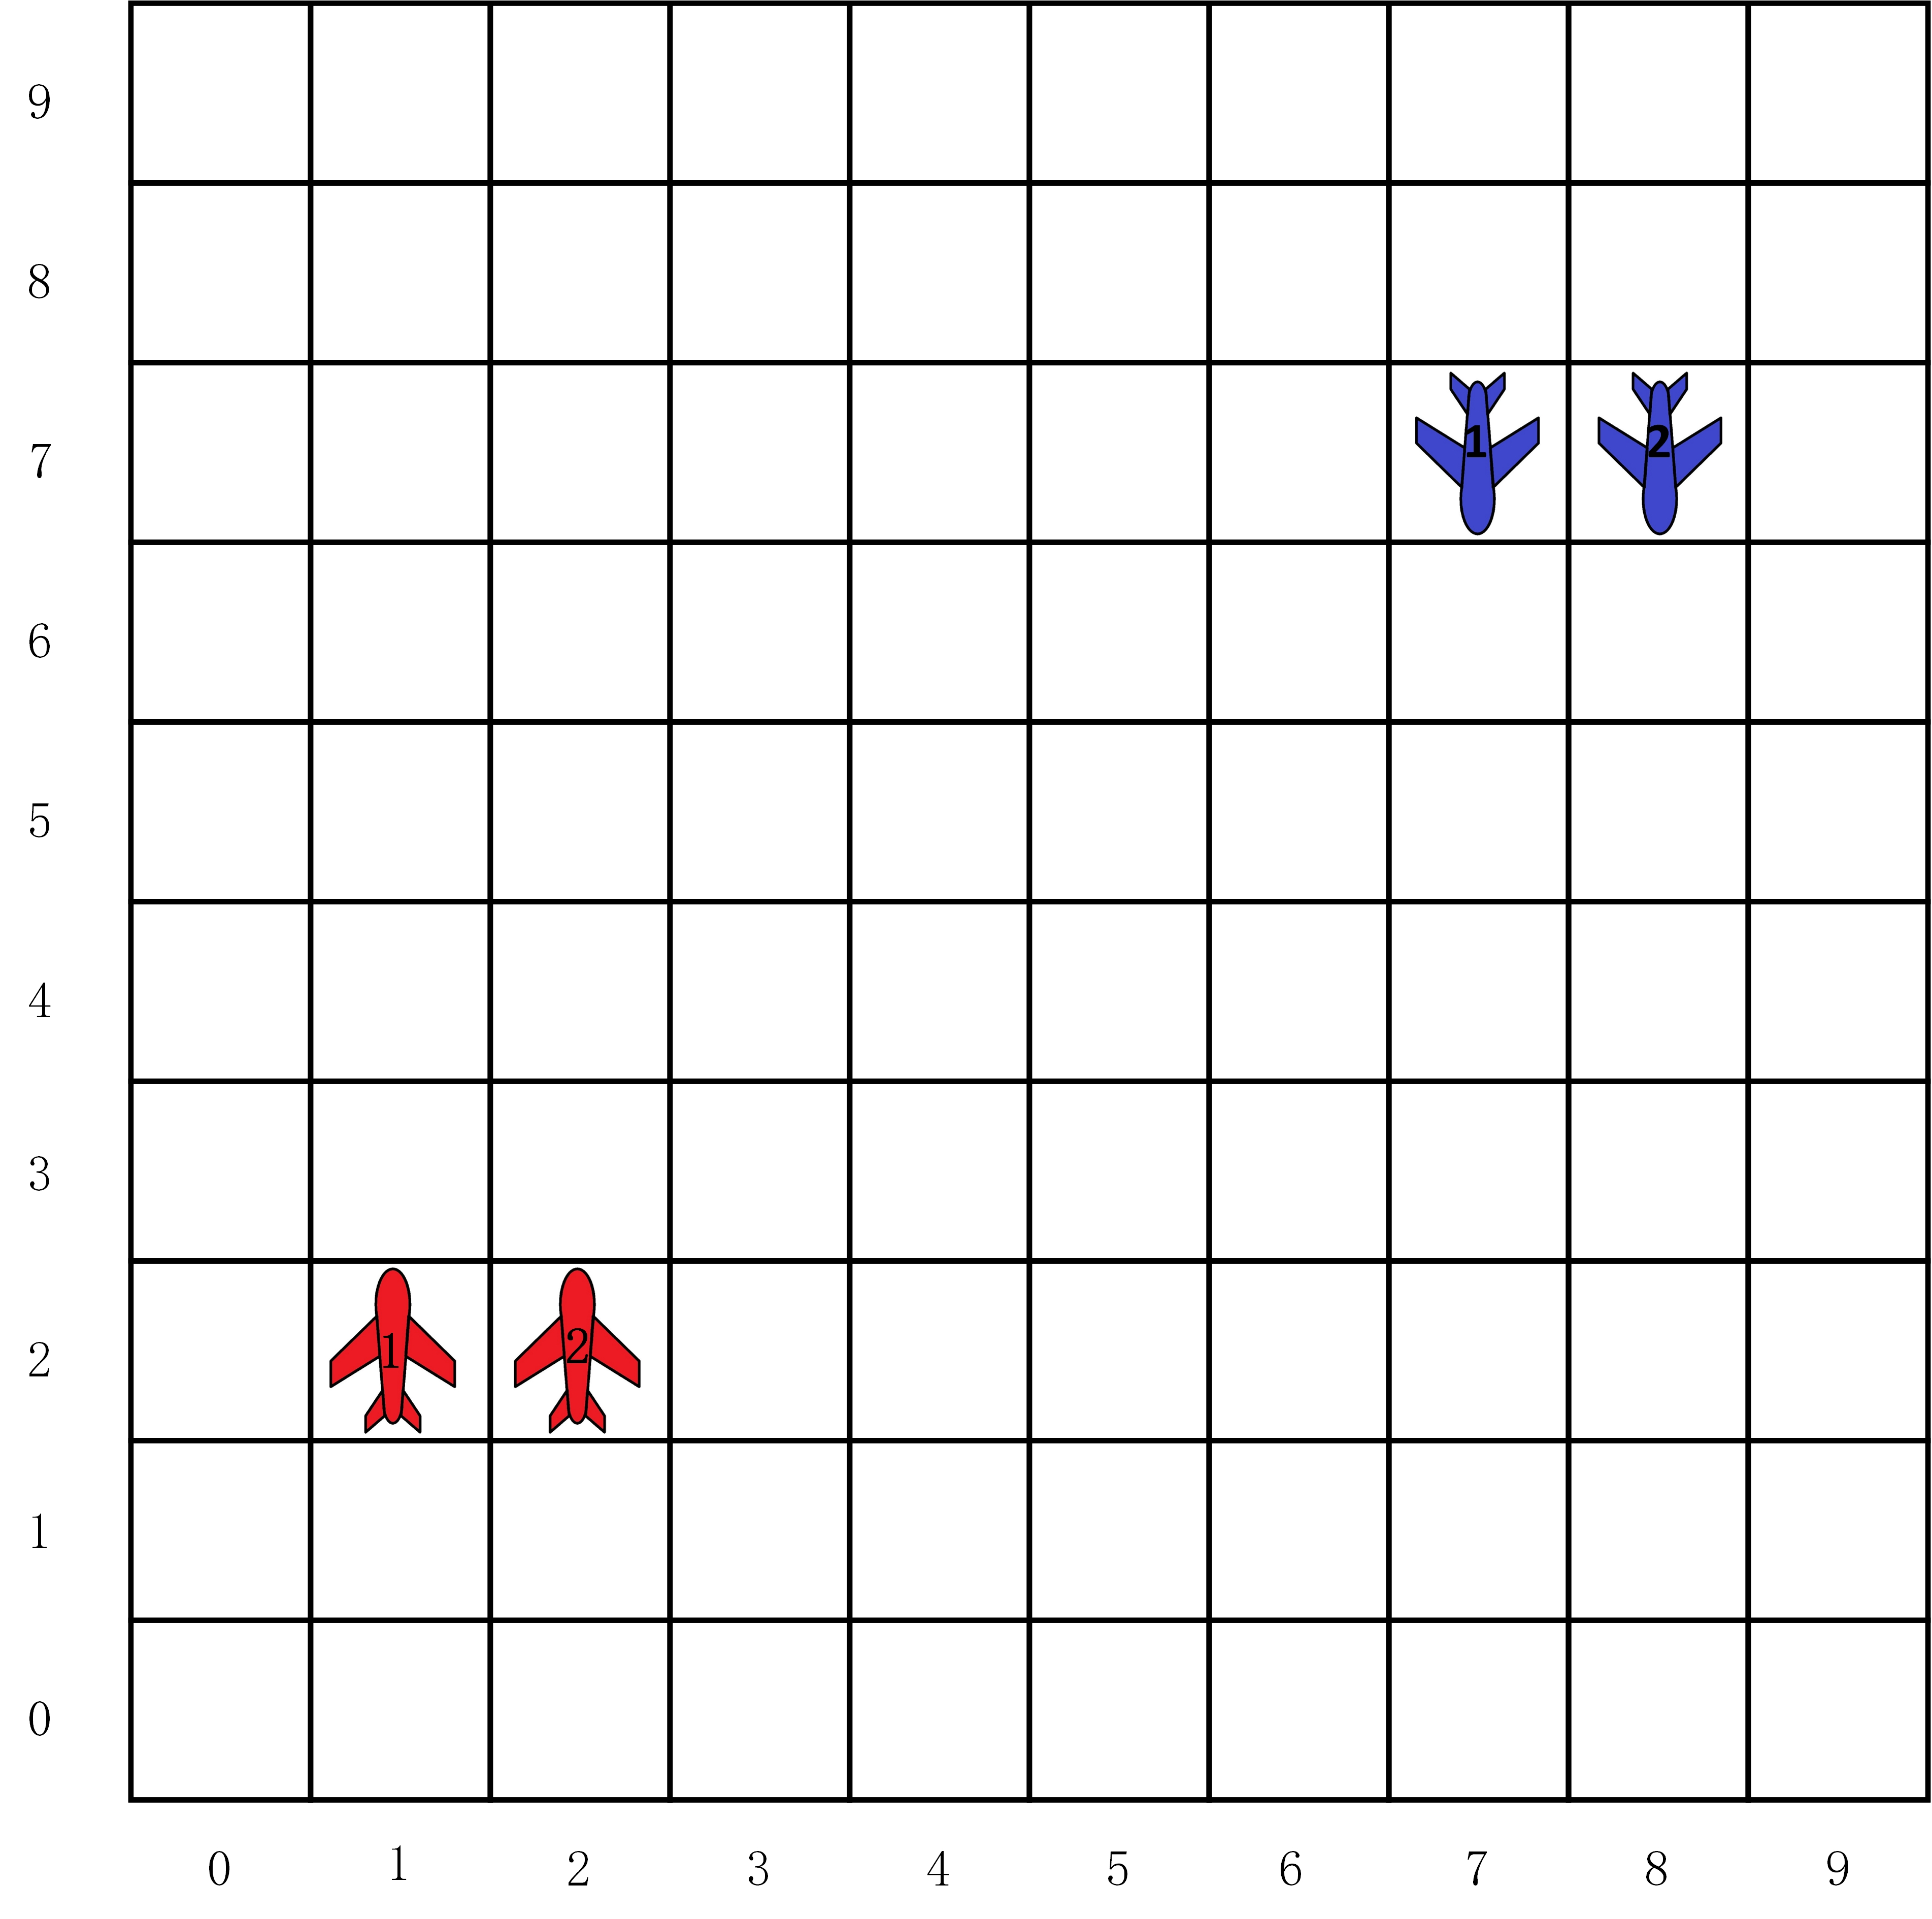
\includegraphics[width=0.45\hsize,height=0.45\hsize]{example/feijichushiweizhi.jpg}}
	\hspace{0.5em}
	\subcaptionbox{\label{fig:duoduiduo1-2:b}}
	{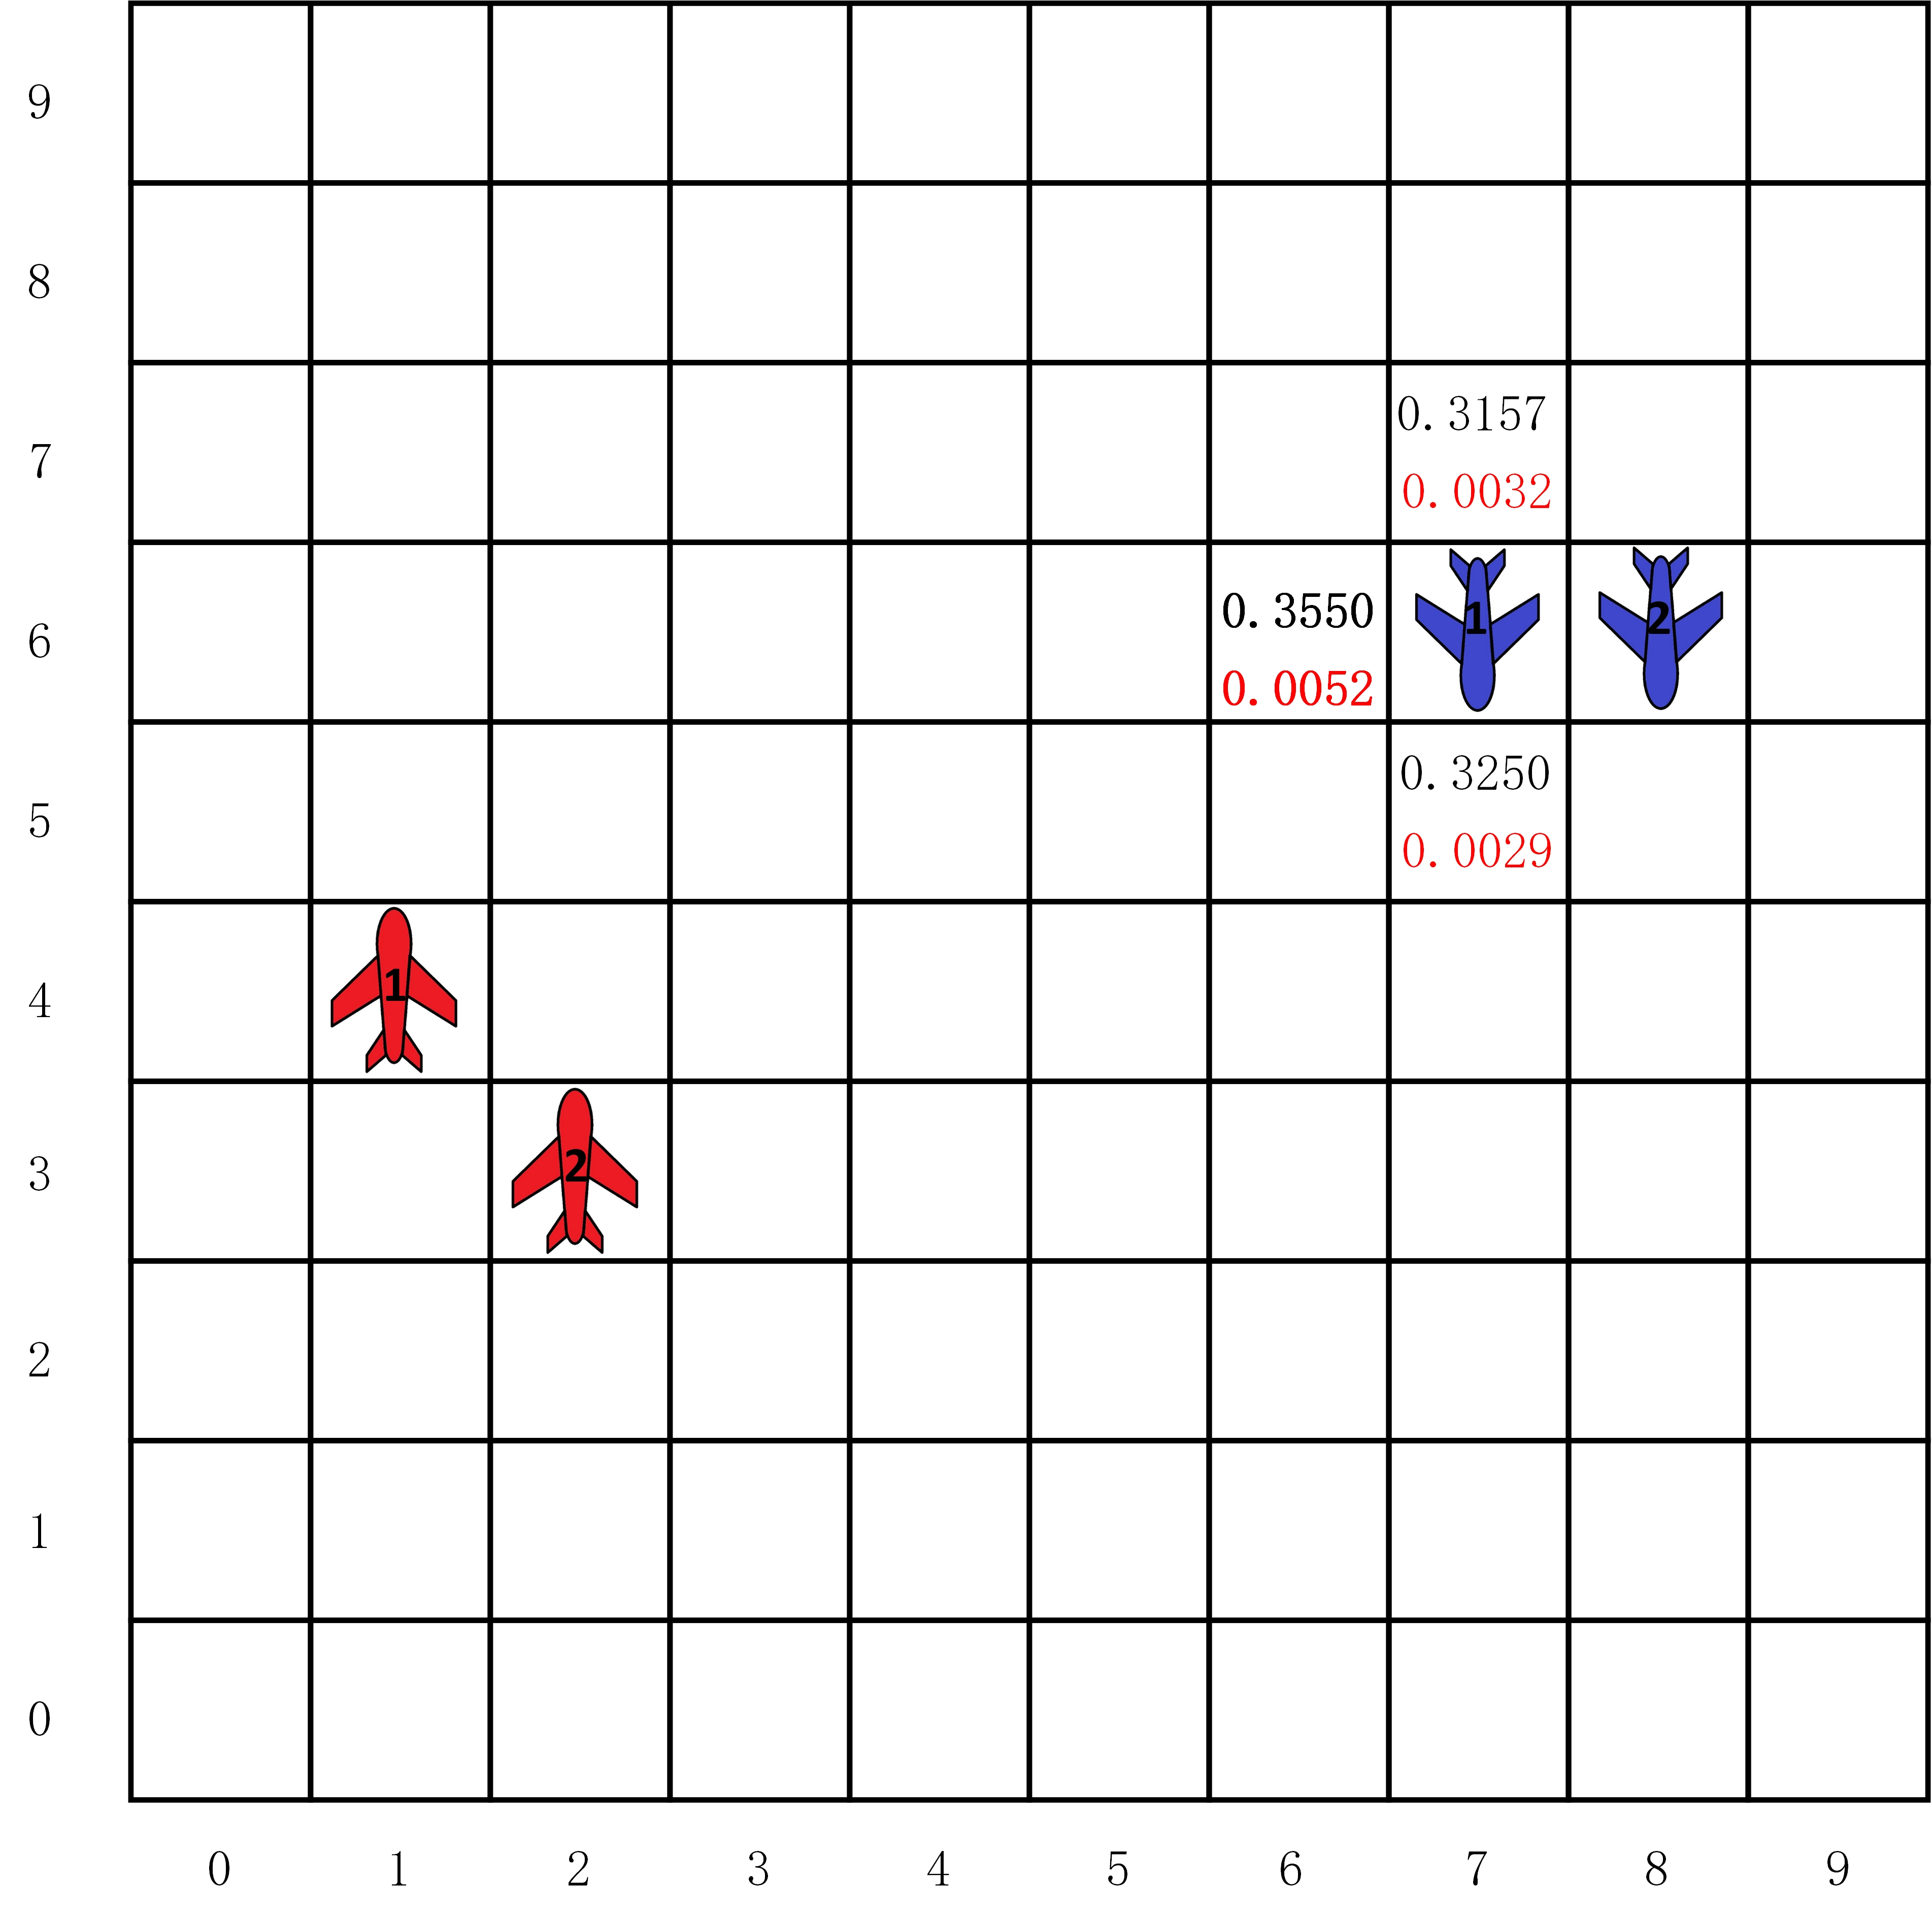
\includegraphics[width=0.45\hsize,height=0.45\hsize]{example/feijierduier2.jpg}}
	\bicaption[二对二初始位置示意图]
	{二对二初始位置示意图}
	{Schematic diagram of initial position between 4 agents.}
	\label{fig:duoduiduo1-2}
\end{figure}
\begin{figure}[!htbp]
	\centering
	\subcaptionbox{\label{fig2:fig:duoduiduo3-6:a}}
	{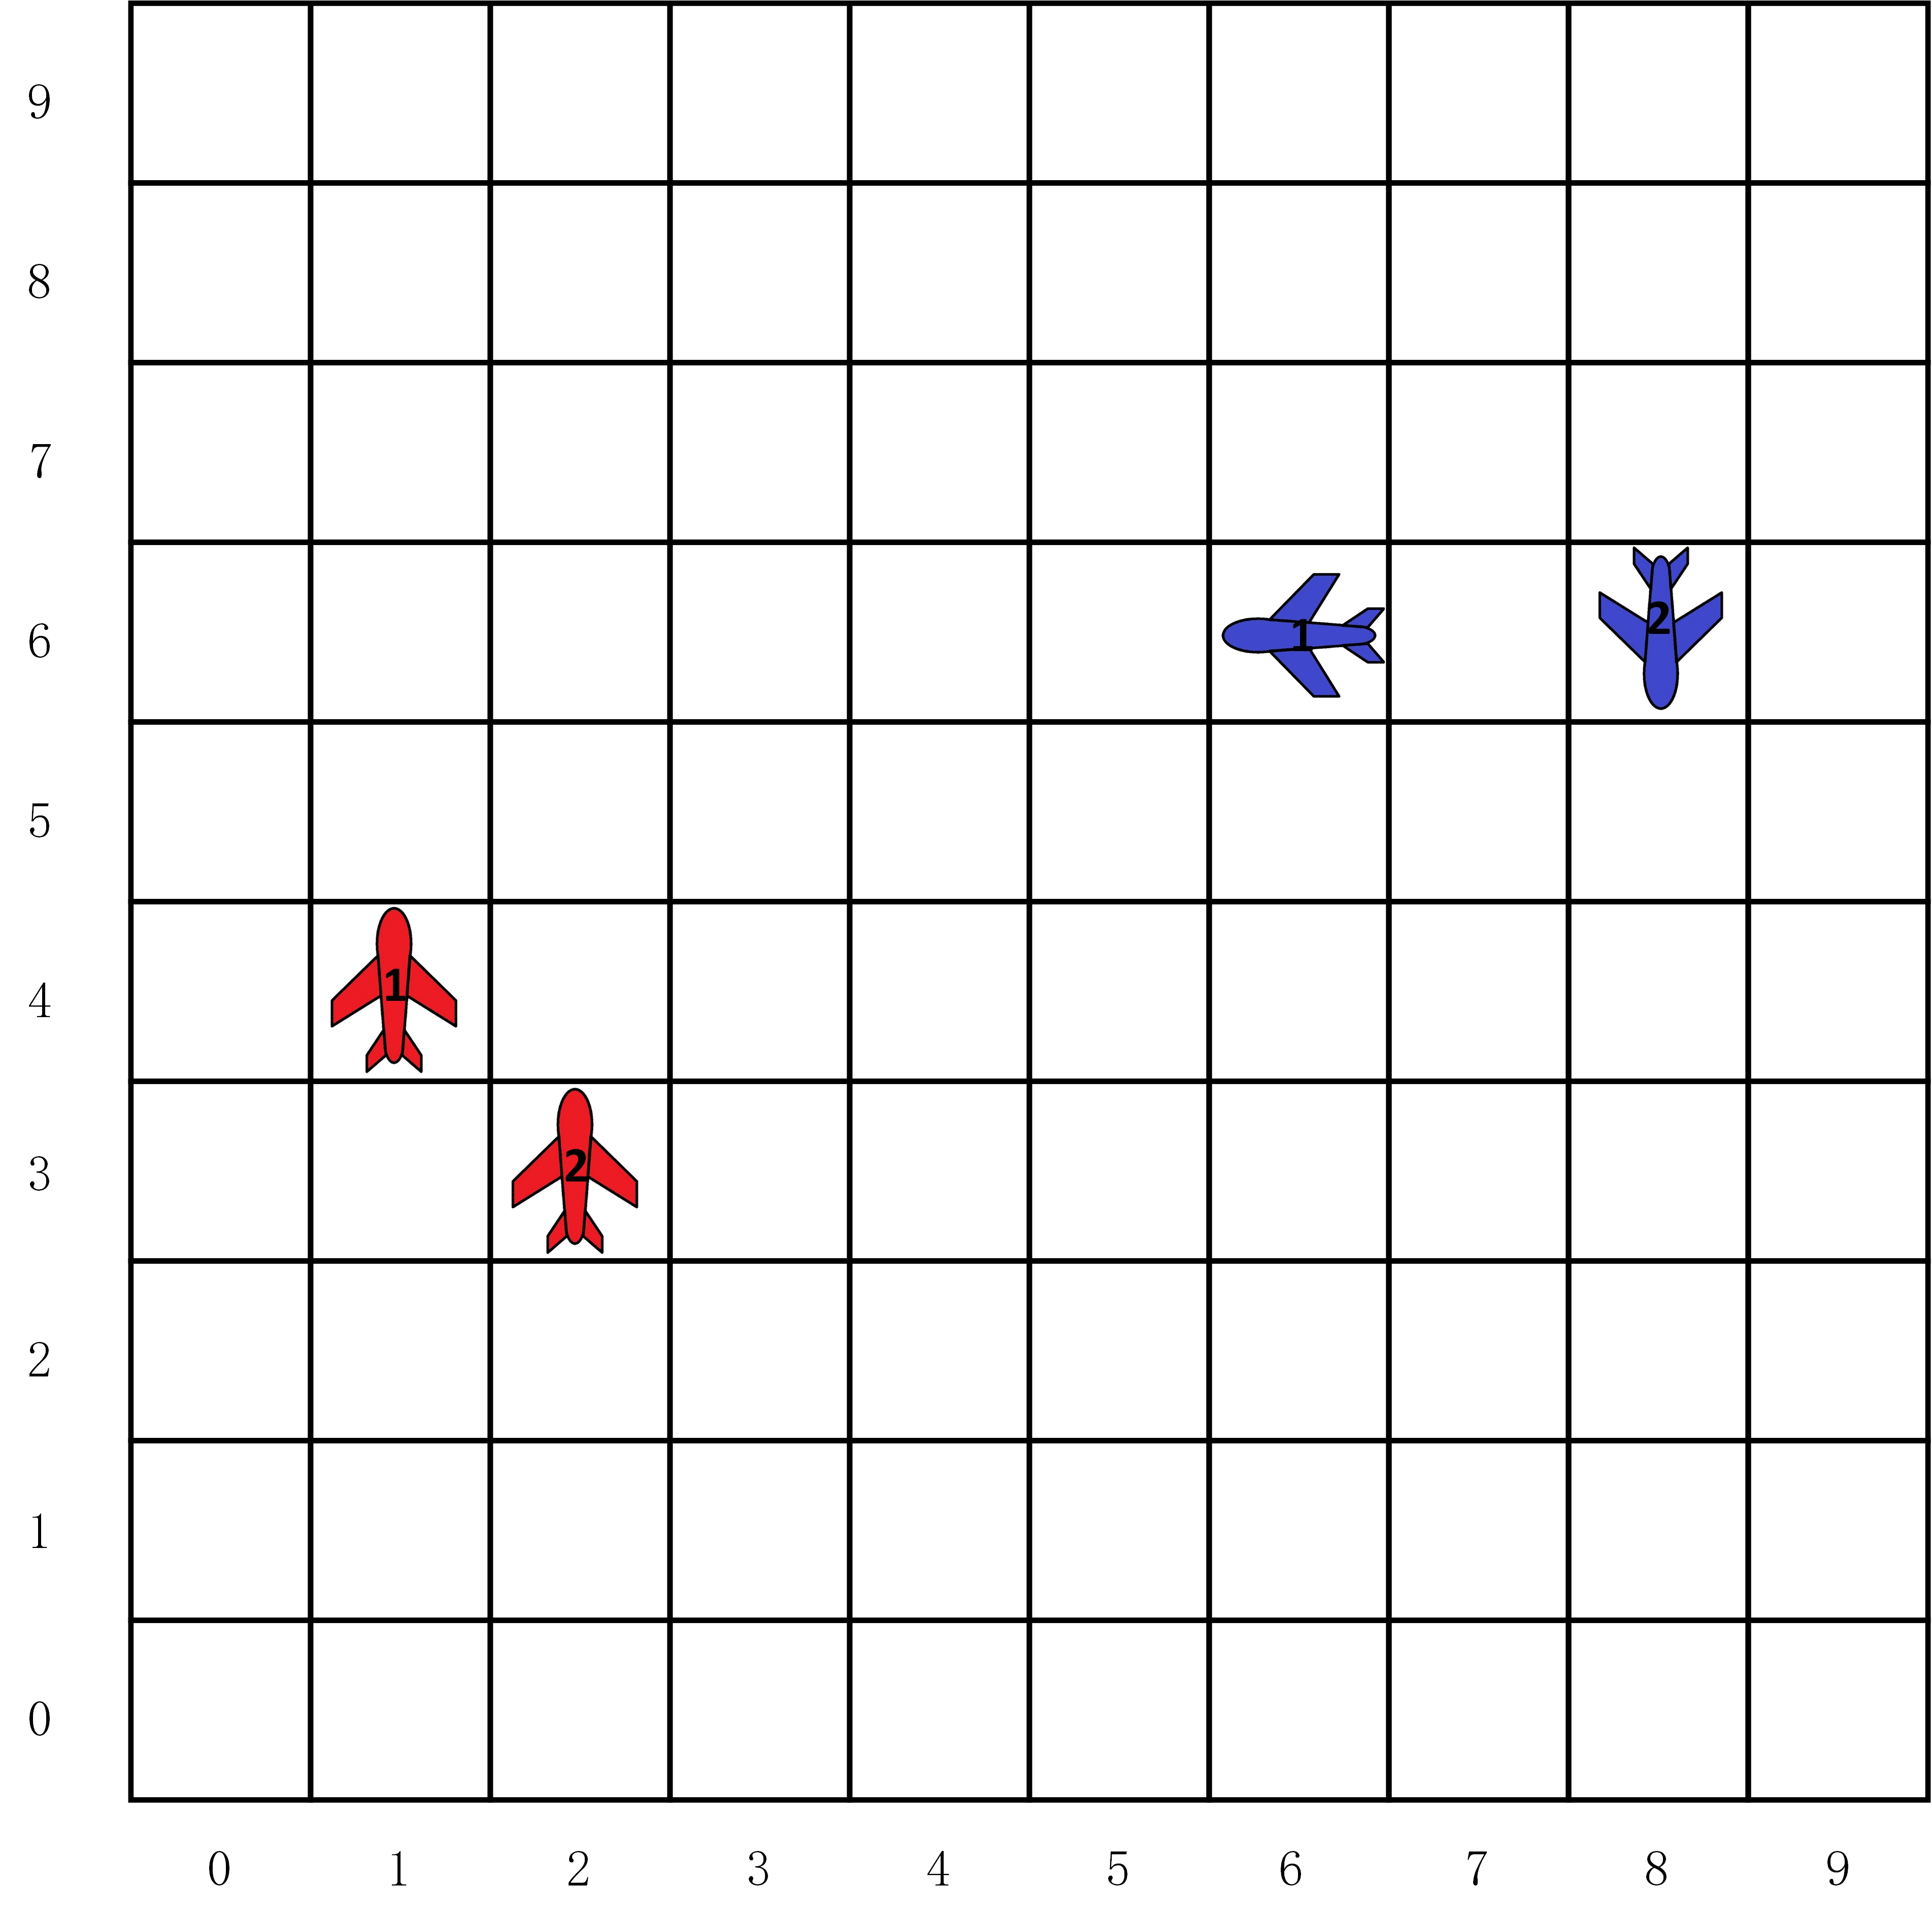
\includegraphics[width=0.45\hsize,height=0.45\hsize]{example/feijierduier3.jpg}}
	\hspace{0.5em}
	\subcaptionbox{\label{fig:duoduiduo3-6:b}}
	{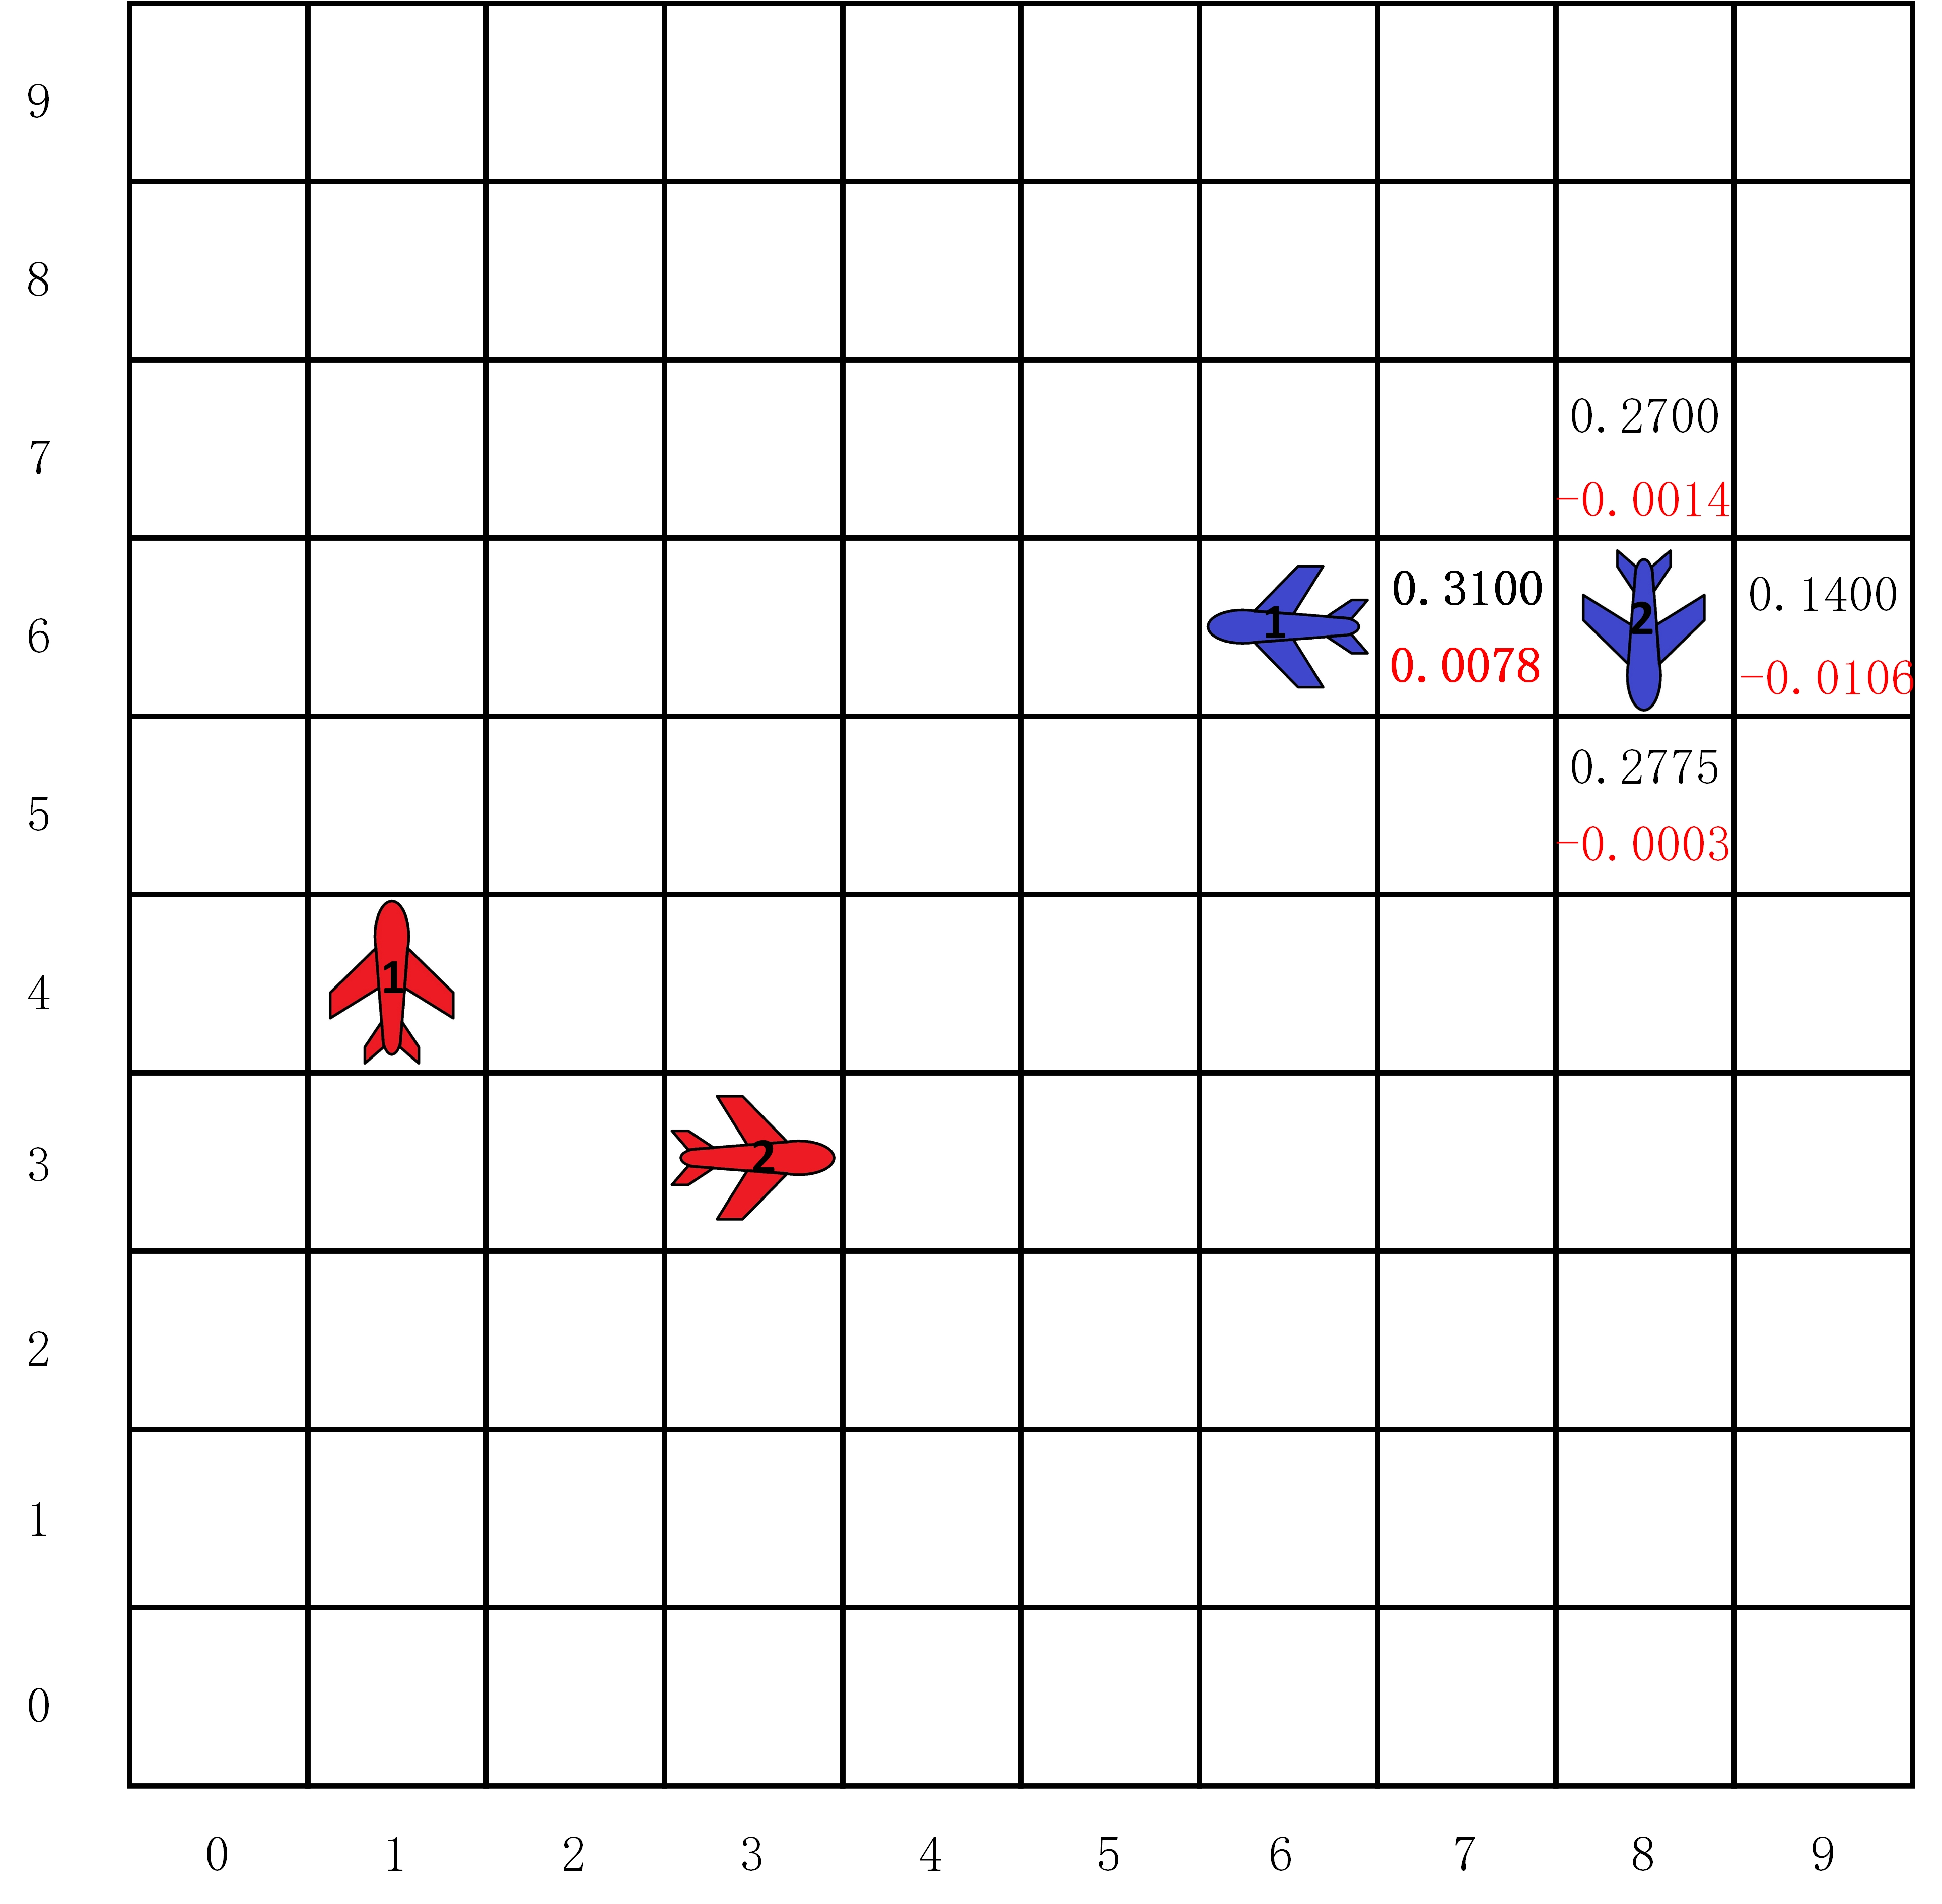
\includegraphics[width=0.45\hsize,height=0.45\hsize]{example/feijierduier4.jpg}}
	\newline
	\centering
	\subcaptionbox{\label{fig:duoduiduo3-6:c}}
	{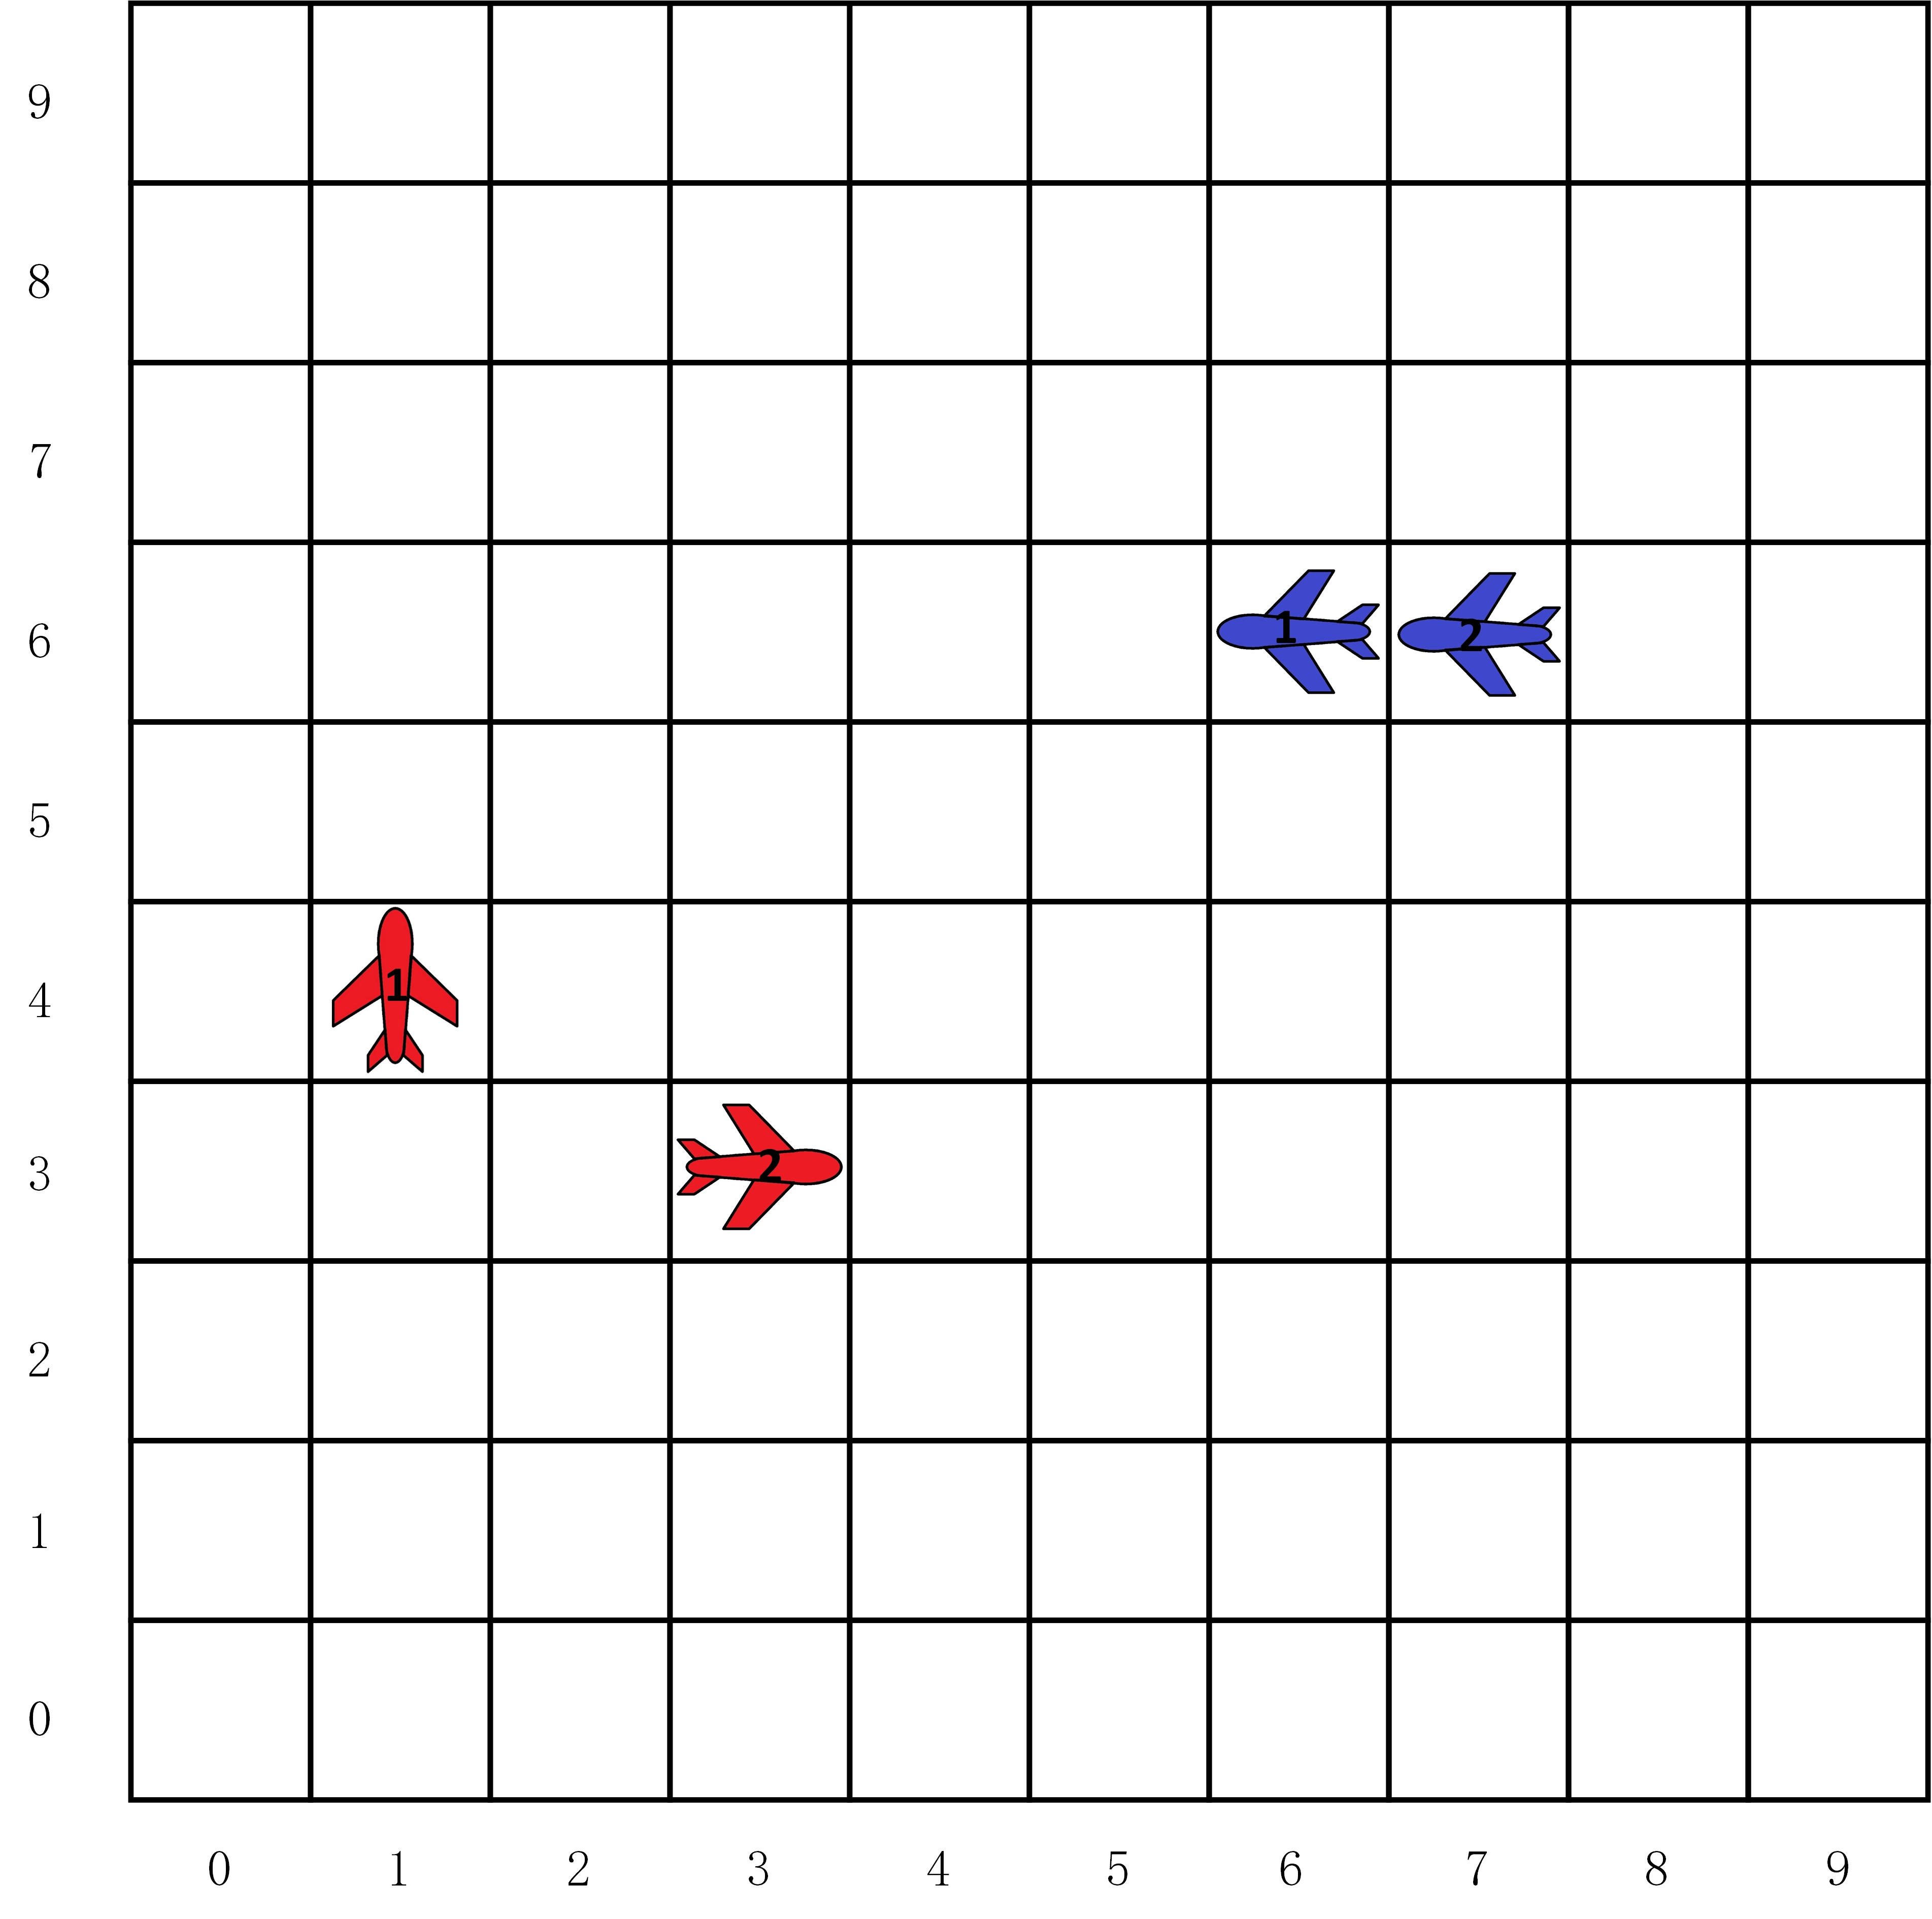
\includegraphics[width=0.45\hsize,height=0.45\hsize]{example/feijierduier5.jpg}}
	\hspace{0.5em}
	\subcaptionbox{\label{fig:duoduiduo3-6:d}}
	{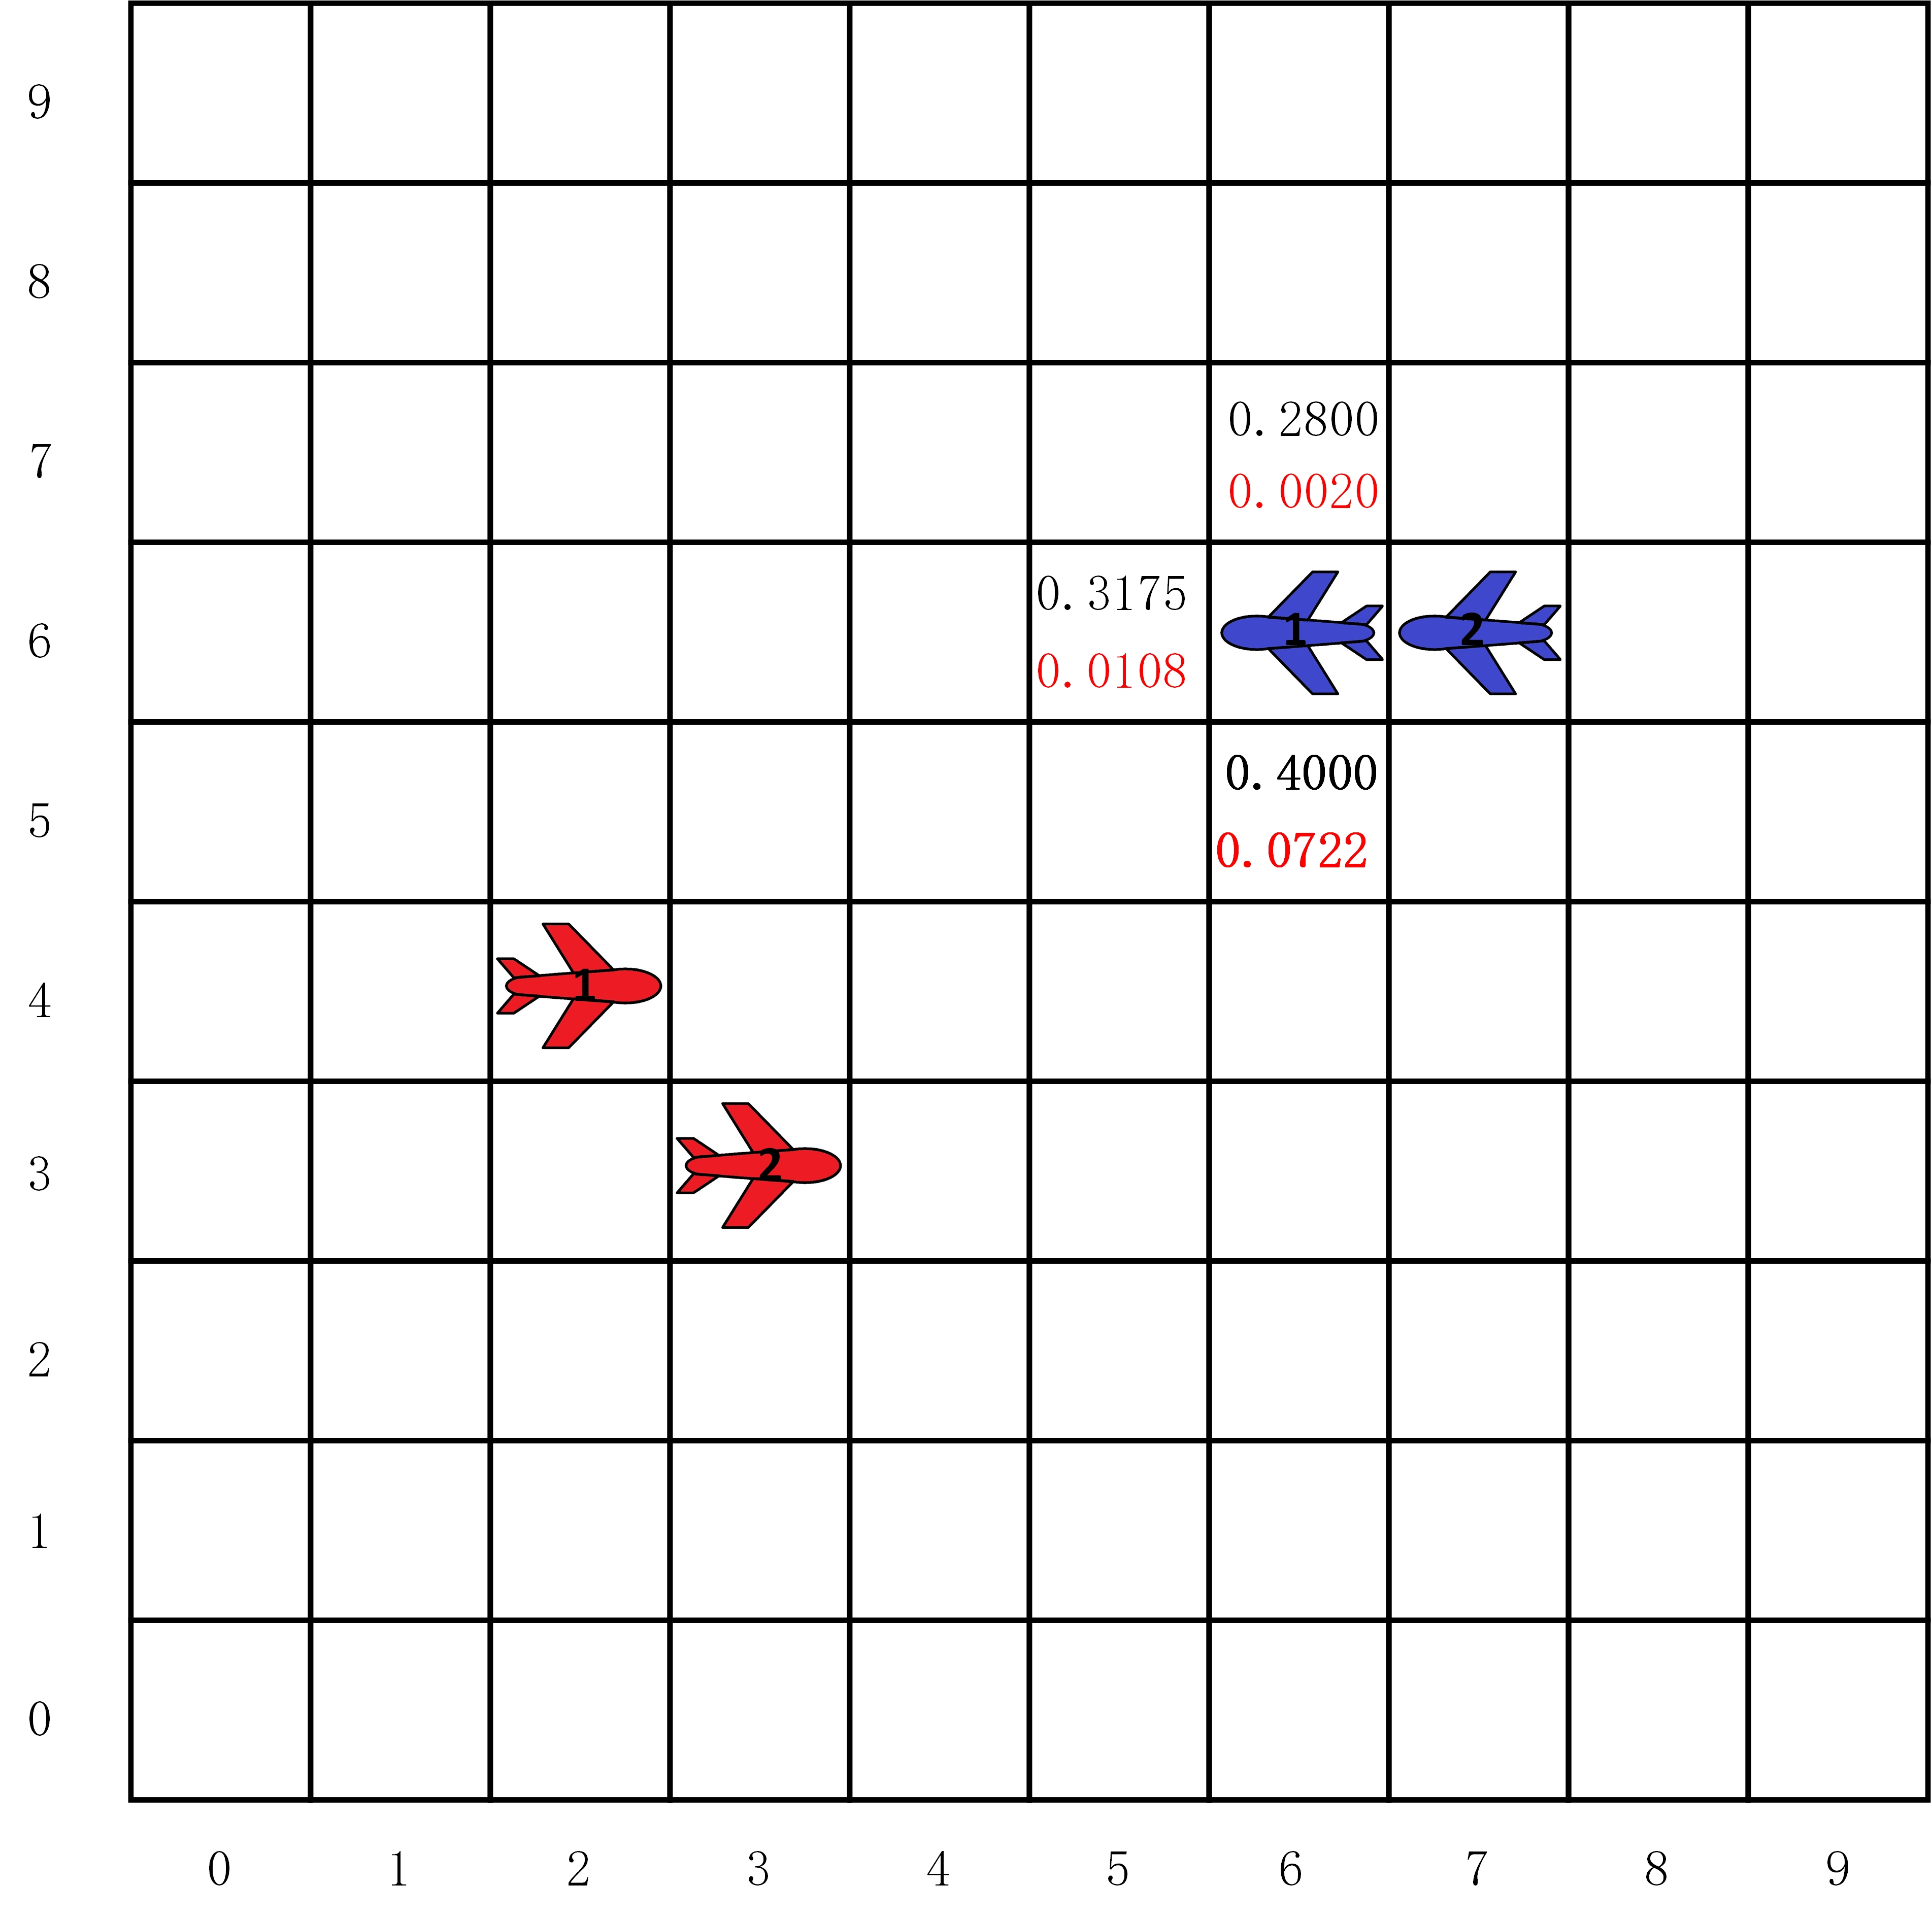
\includegraphics[width=0.45\hsize,height=0.45\hsize]{example/feijierduier6.jpg}}
	\bicaption[二对二人机对弈过程图示(1)]
	{二对二人机对弈过程图示}
	{Diagram of man-machine game process(1).}
	\label{fig:duoduiduo3-6}
\end{figure}
\begin{figure}[!htbp]
	\centering
	\subcaptionbox{\label{fig:duoduiduo9-10:a}}
	{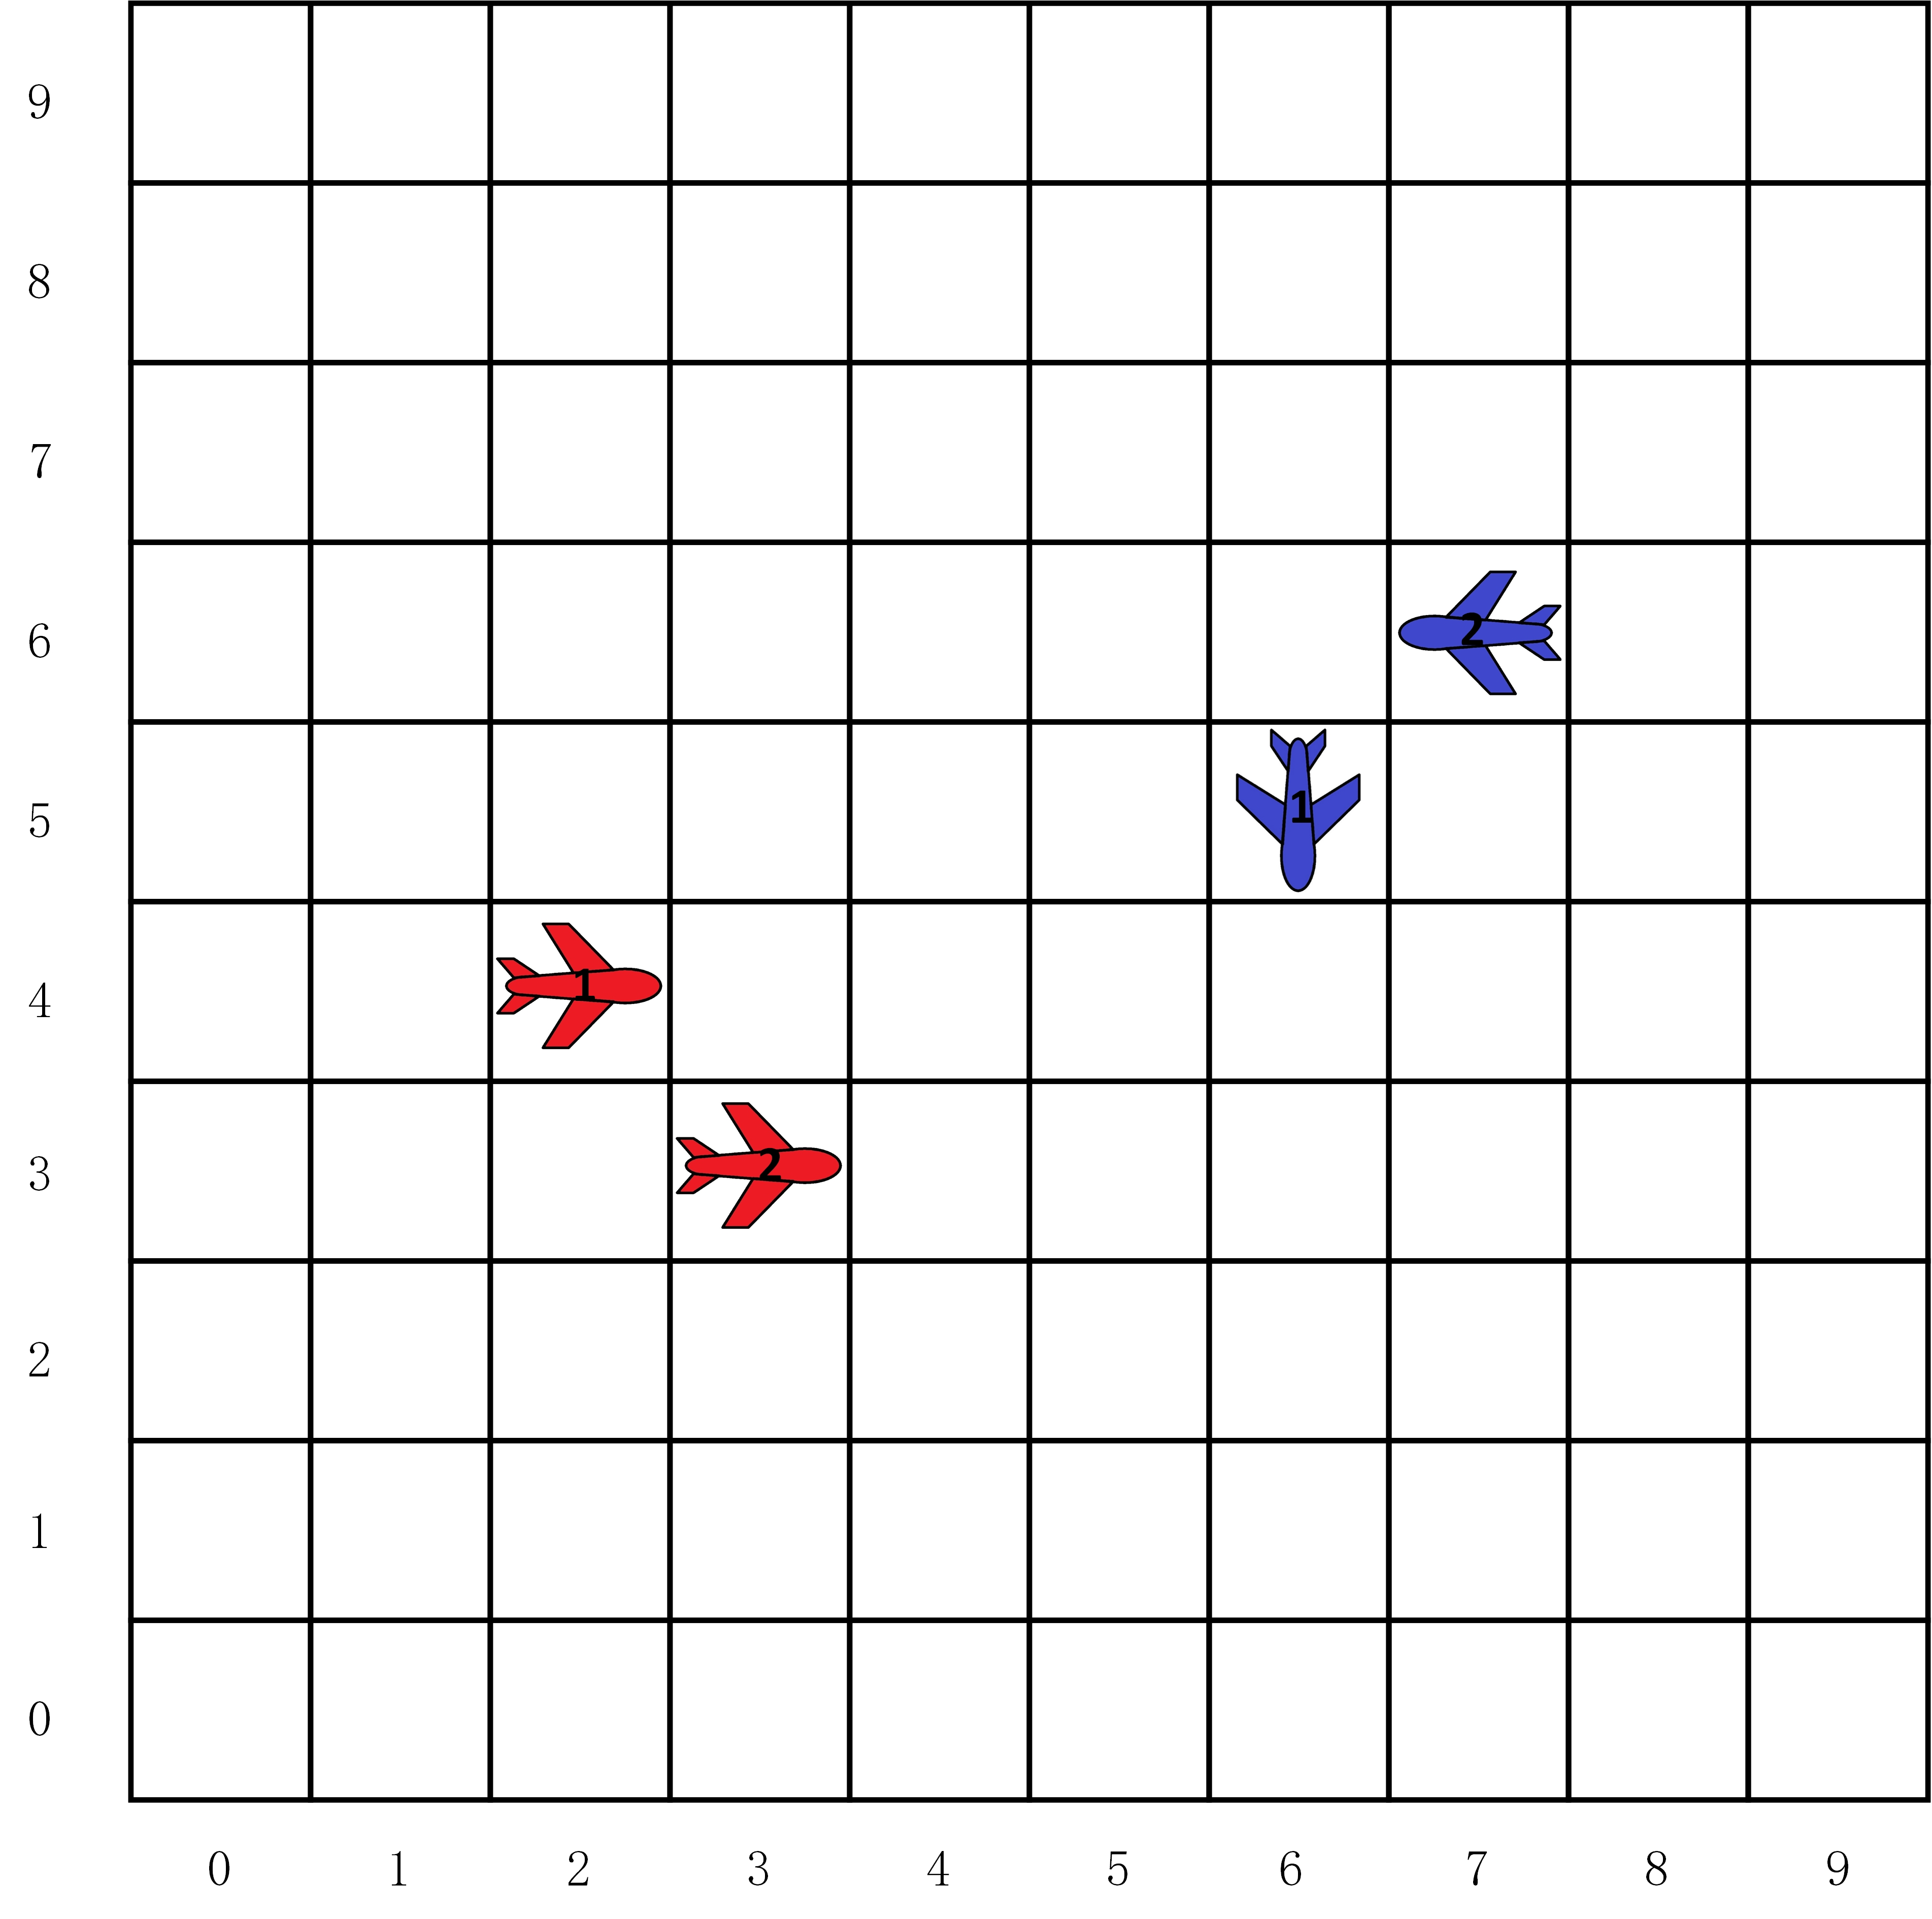
\includegraphics[width=0.45\hsize,height=0.45\hsize]{example/feijierduier7.jpg}}
	\hspace{0.5em}
	\subcaptionbox{\label{fig:duoduiduo9-10:b}}
	{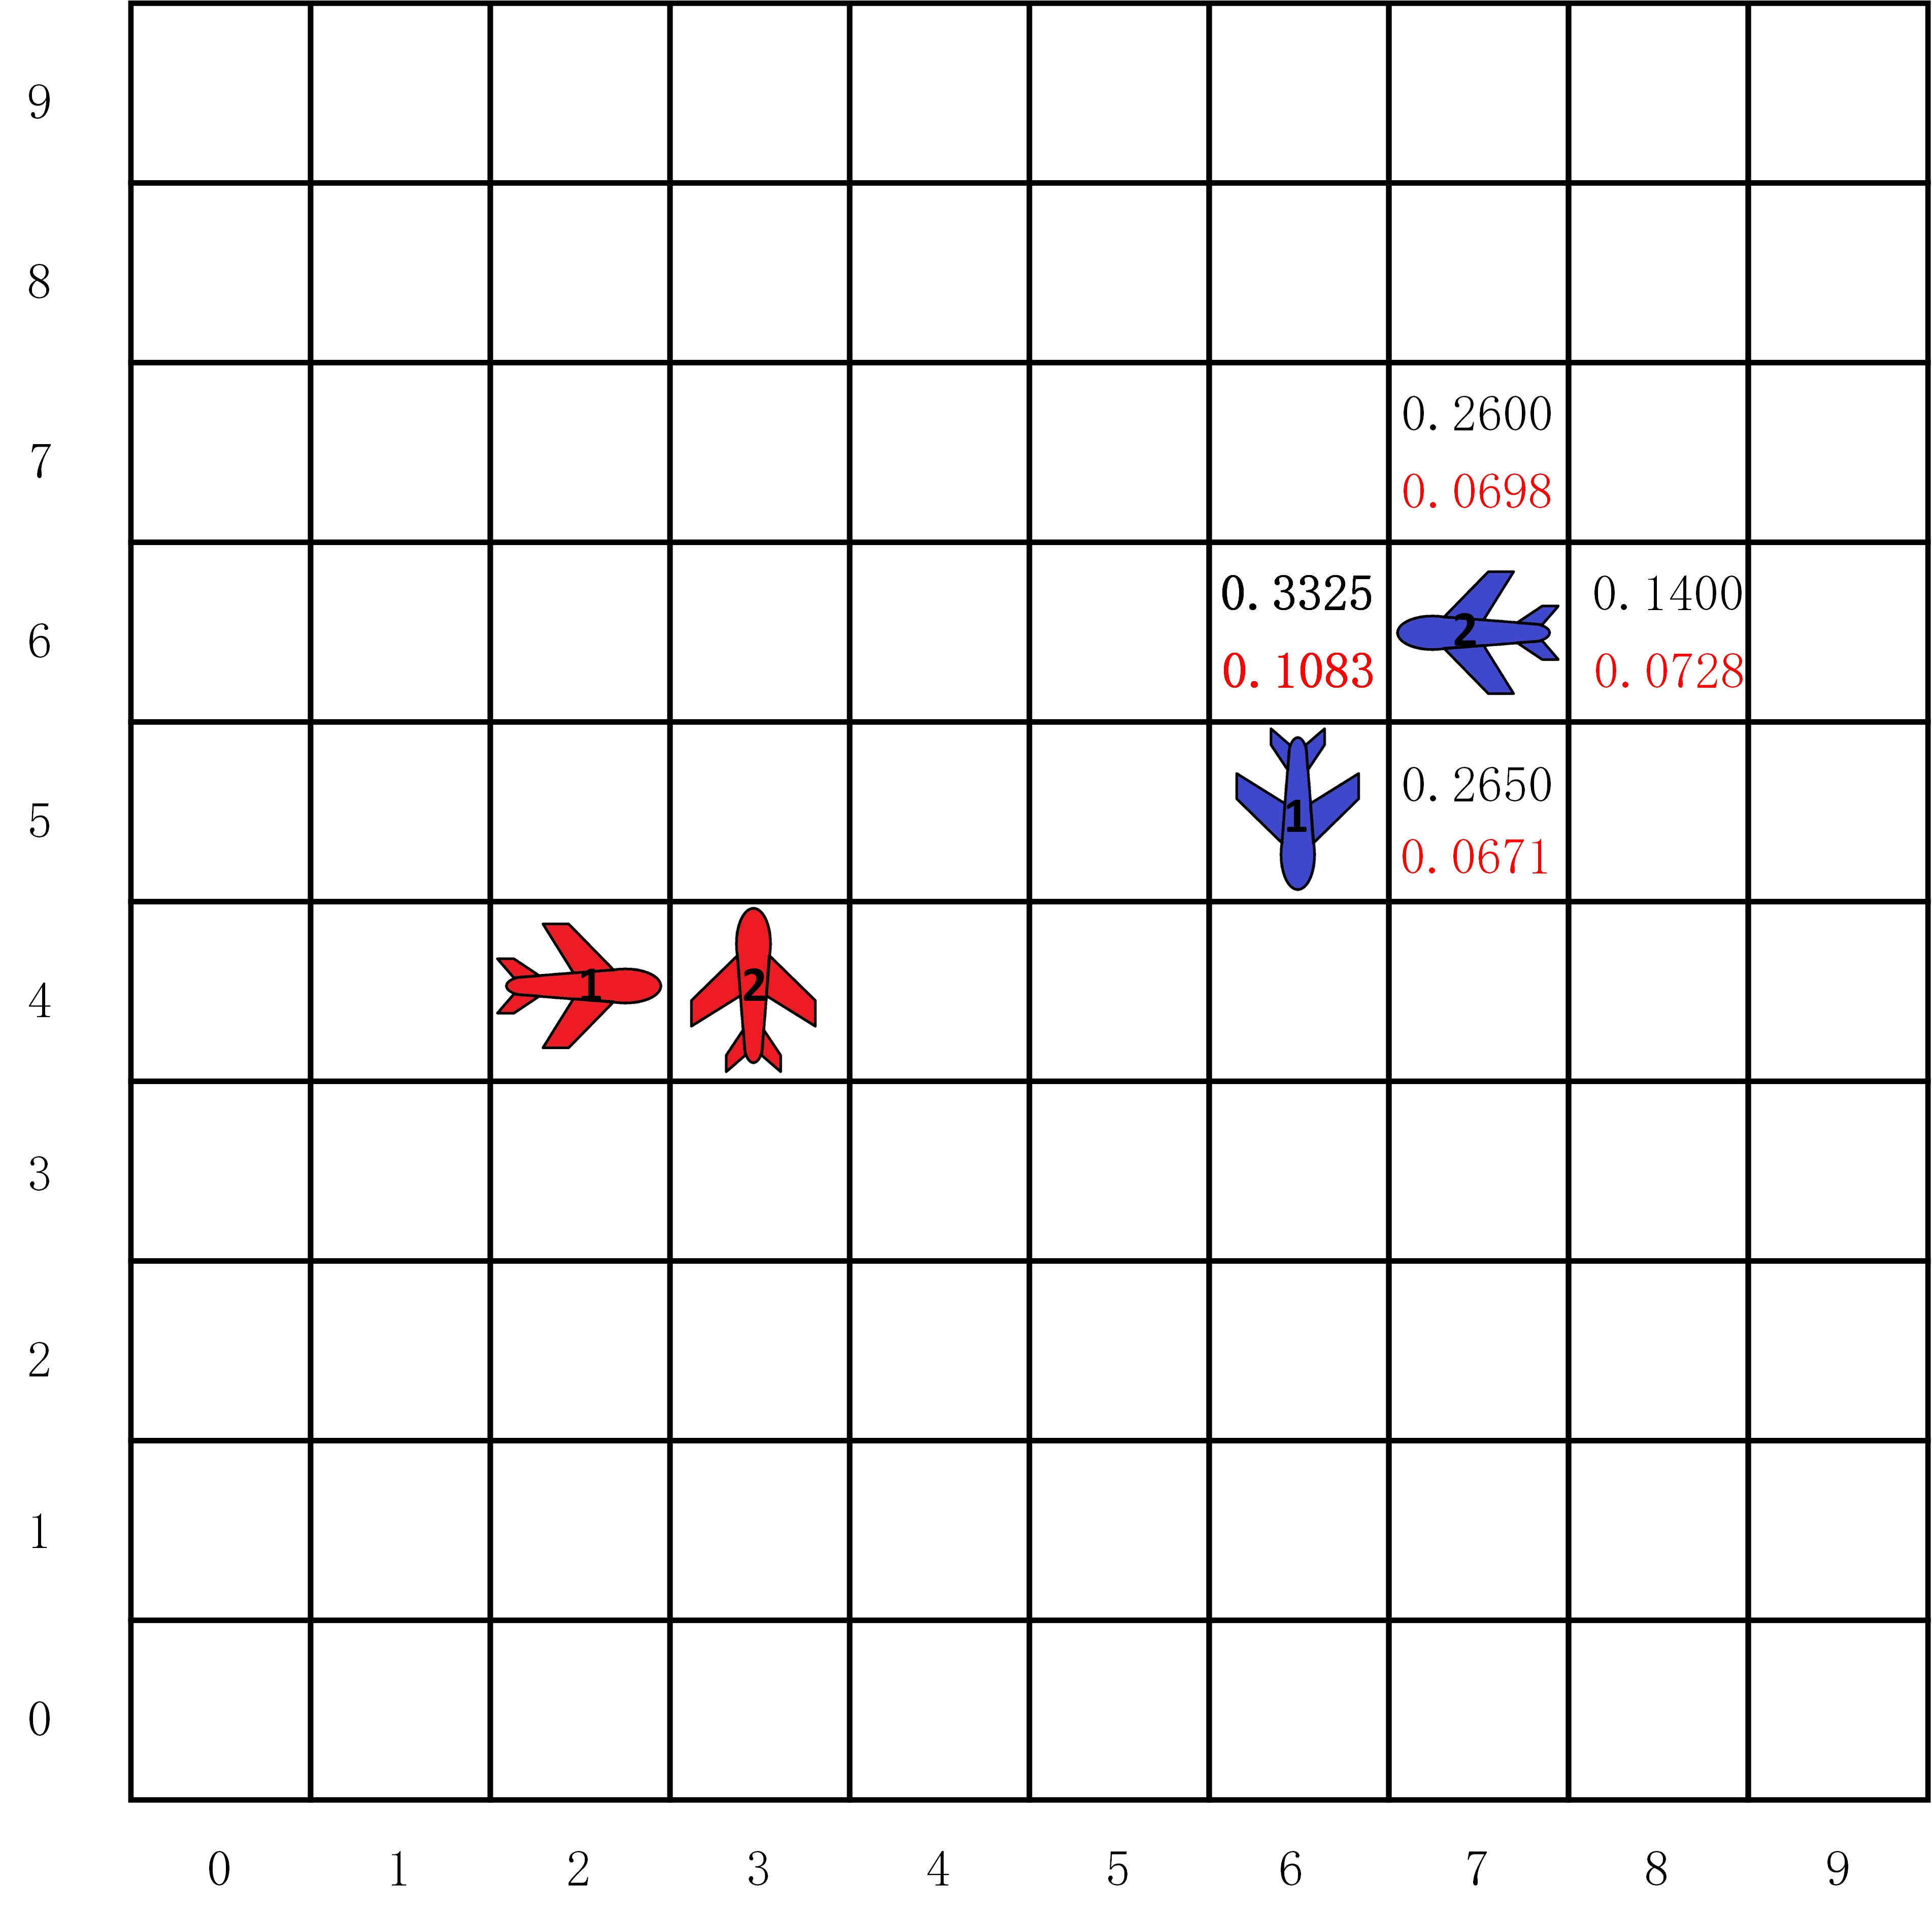
\includegraphics[width=0.45\hsize,height=0.45\hsize]{example/feijierduier8.jpg}}
	\newline
	\centering
	\subcaptionbox{\label{fig2:fig:duoduiduo9-10:c}}
	{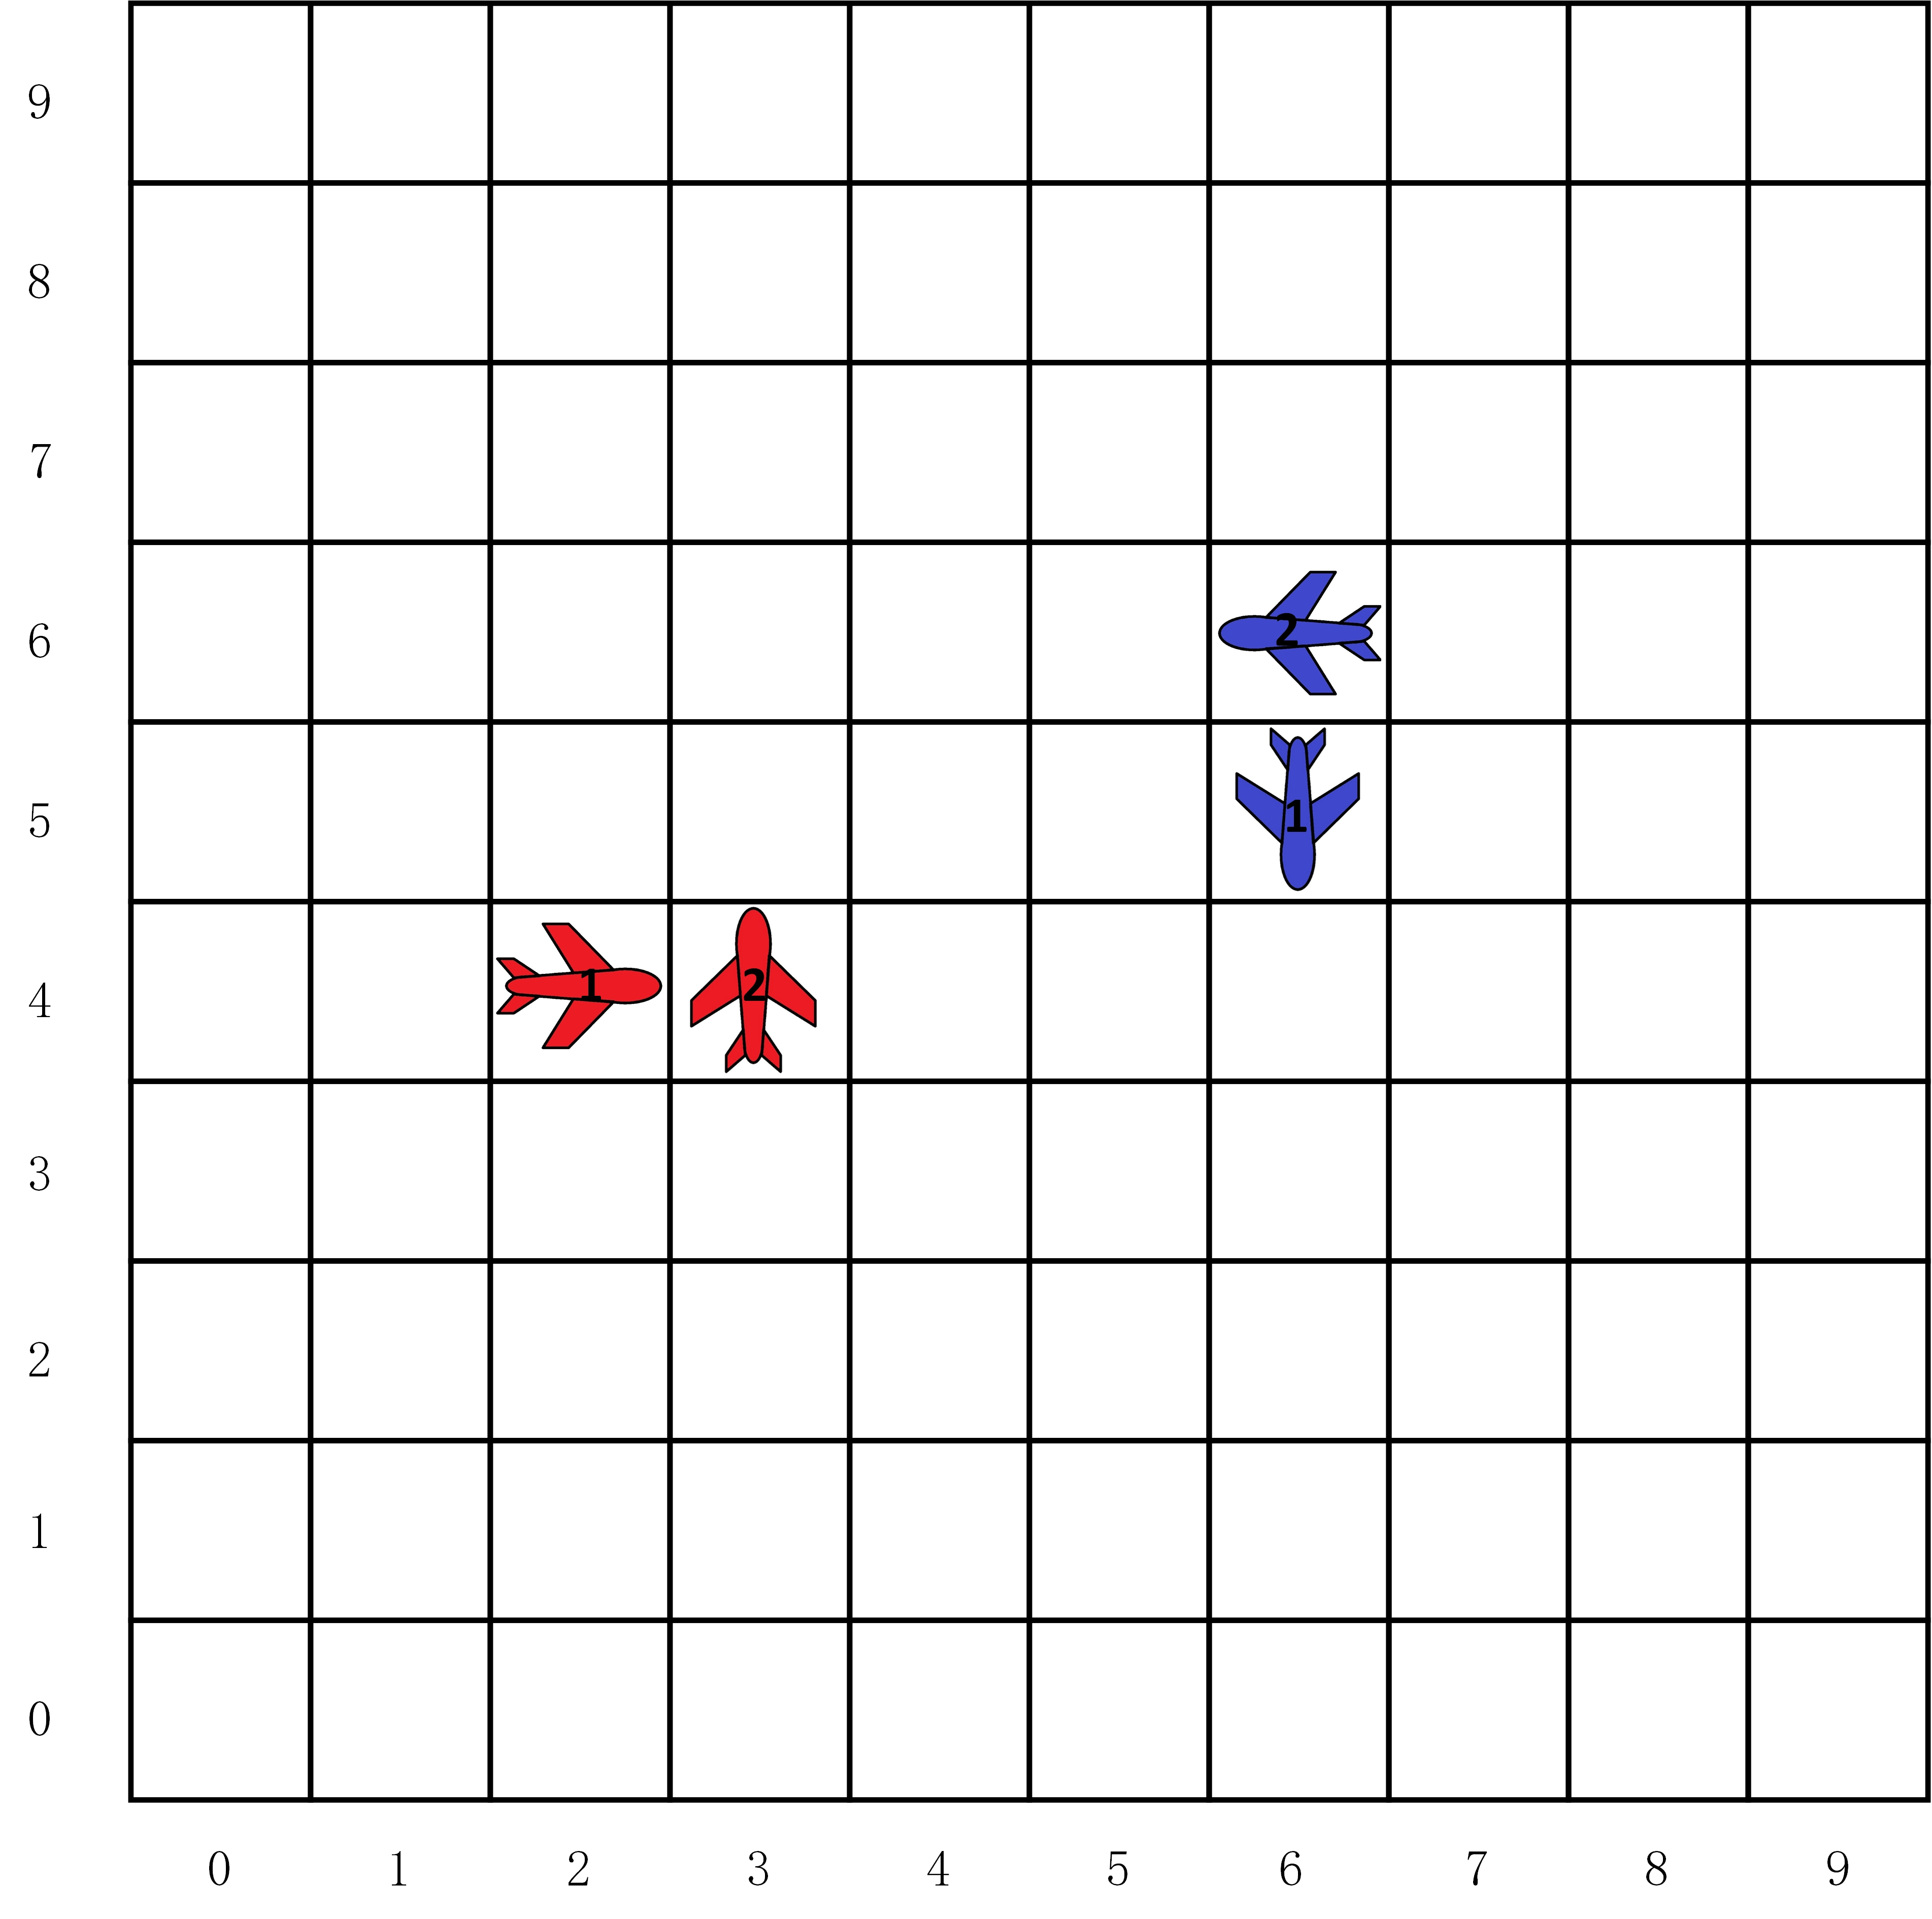
\includegraphics[width=0.45\hsize,height=0.45\hsize]{example/feijierduier9.jpg}}
	\hspace{0.5em}
	\subcaptionbox{\label{fig:duoduiduo9-10:d}}
	{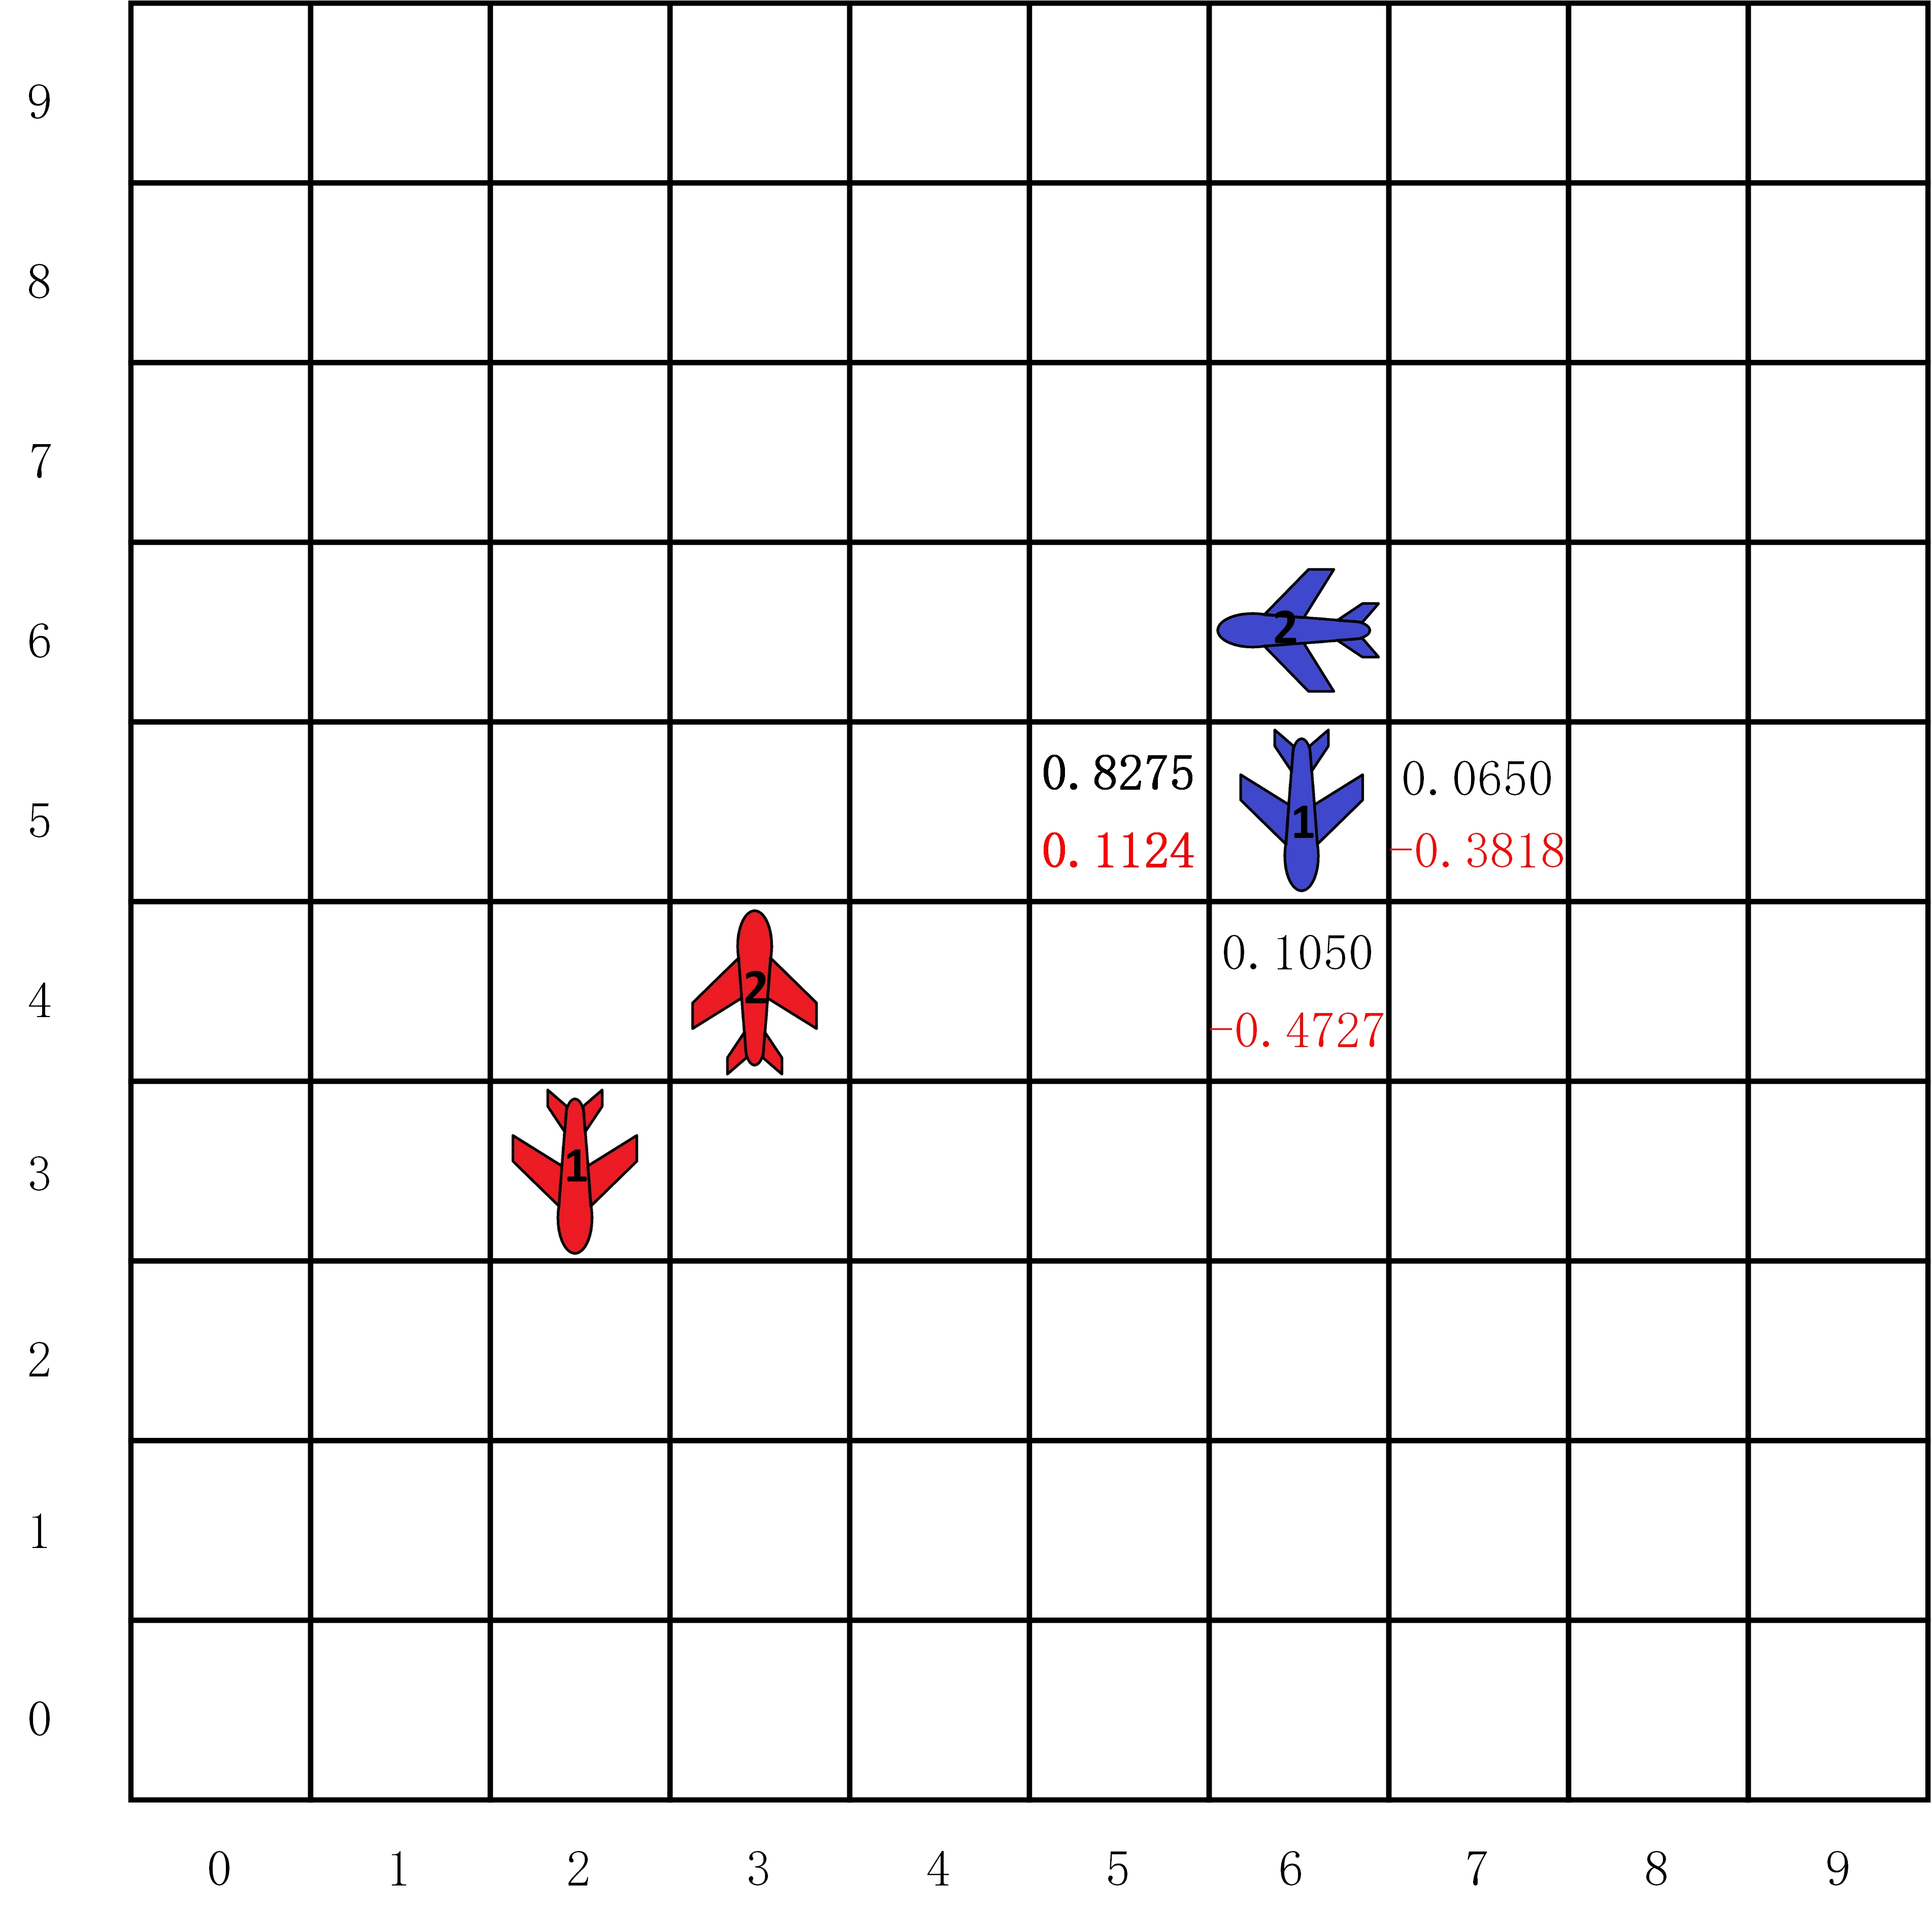
\includegraphics[width=0.45\hsize,height=0.45\hsize]{example/feijierduier10.jpg}}
	\bicaption[二对二人机对弈过程图示(2)]
	{二对二人机对弈过程图示}
	{Diagram of man-machine game process(2).}
	\label{fig:duoduiduo9-10}
\end{figure}
\subsubsection{对弈关系分析}

在队间智能体博弈方面,图\ref{fig2:duoduiduo}分析了当蓝一分别执行向下和向右的动作时红蓝两方的状态关系。通过分别计算蓝一和红一红二智能体之间的状态信息,可以看出当向下和向右移动无法击败敌机,而当执行按照图\ref{fig:duoduiduo3-6:d}策略,选取最大概率的动作向左时状态如图\ref{fig3:duoduiduo}。此时蓝一到达了对红二的最佳攻击位置,击败红二,AI模型获胜。
\begin{figure}[!hpbt]
	\centering
	\subcaptionbox{向下状态\label{fig2:duoduiduo:a}}
	{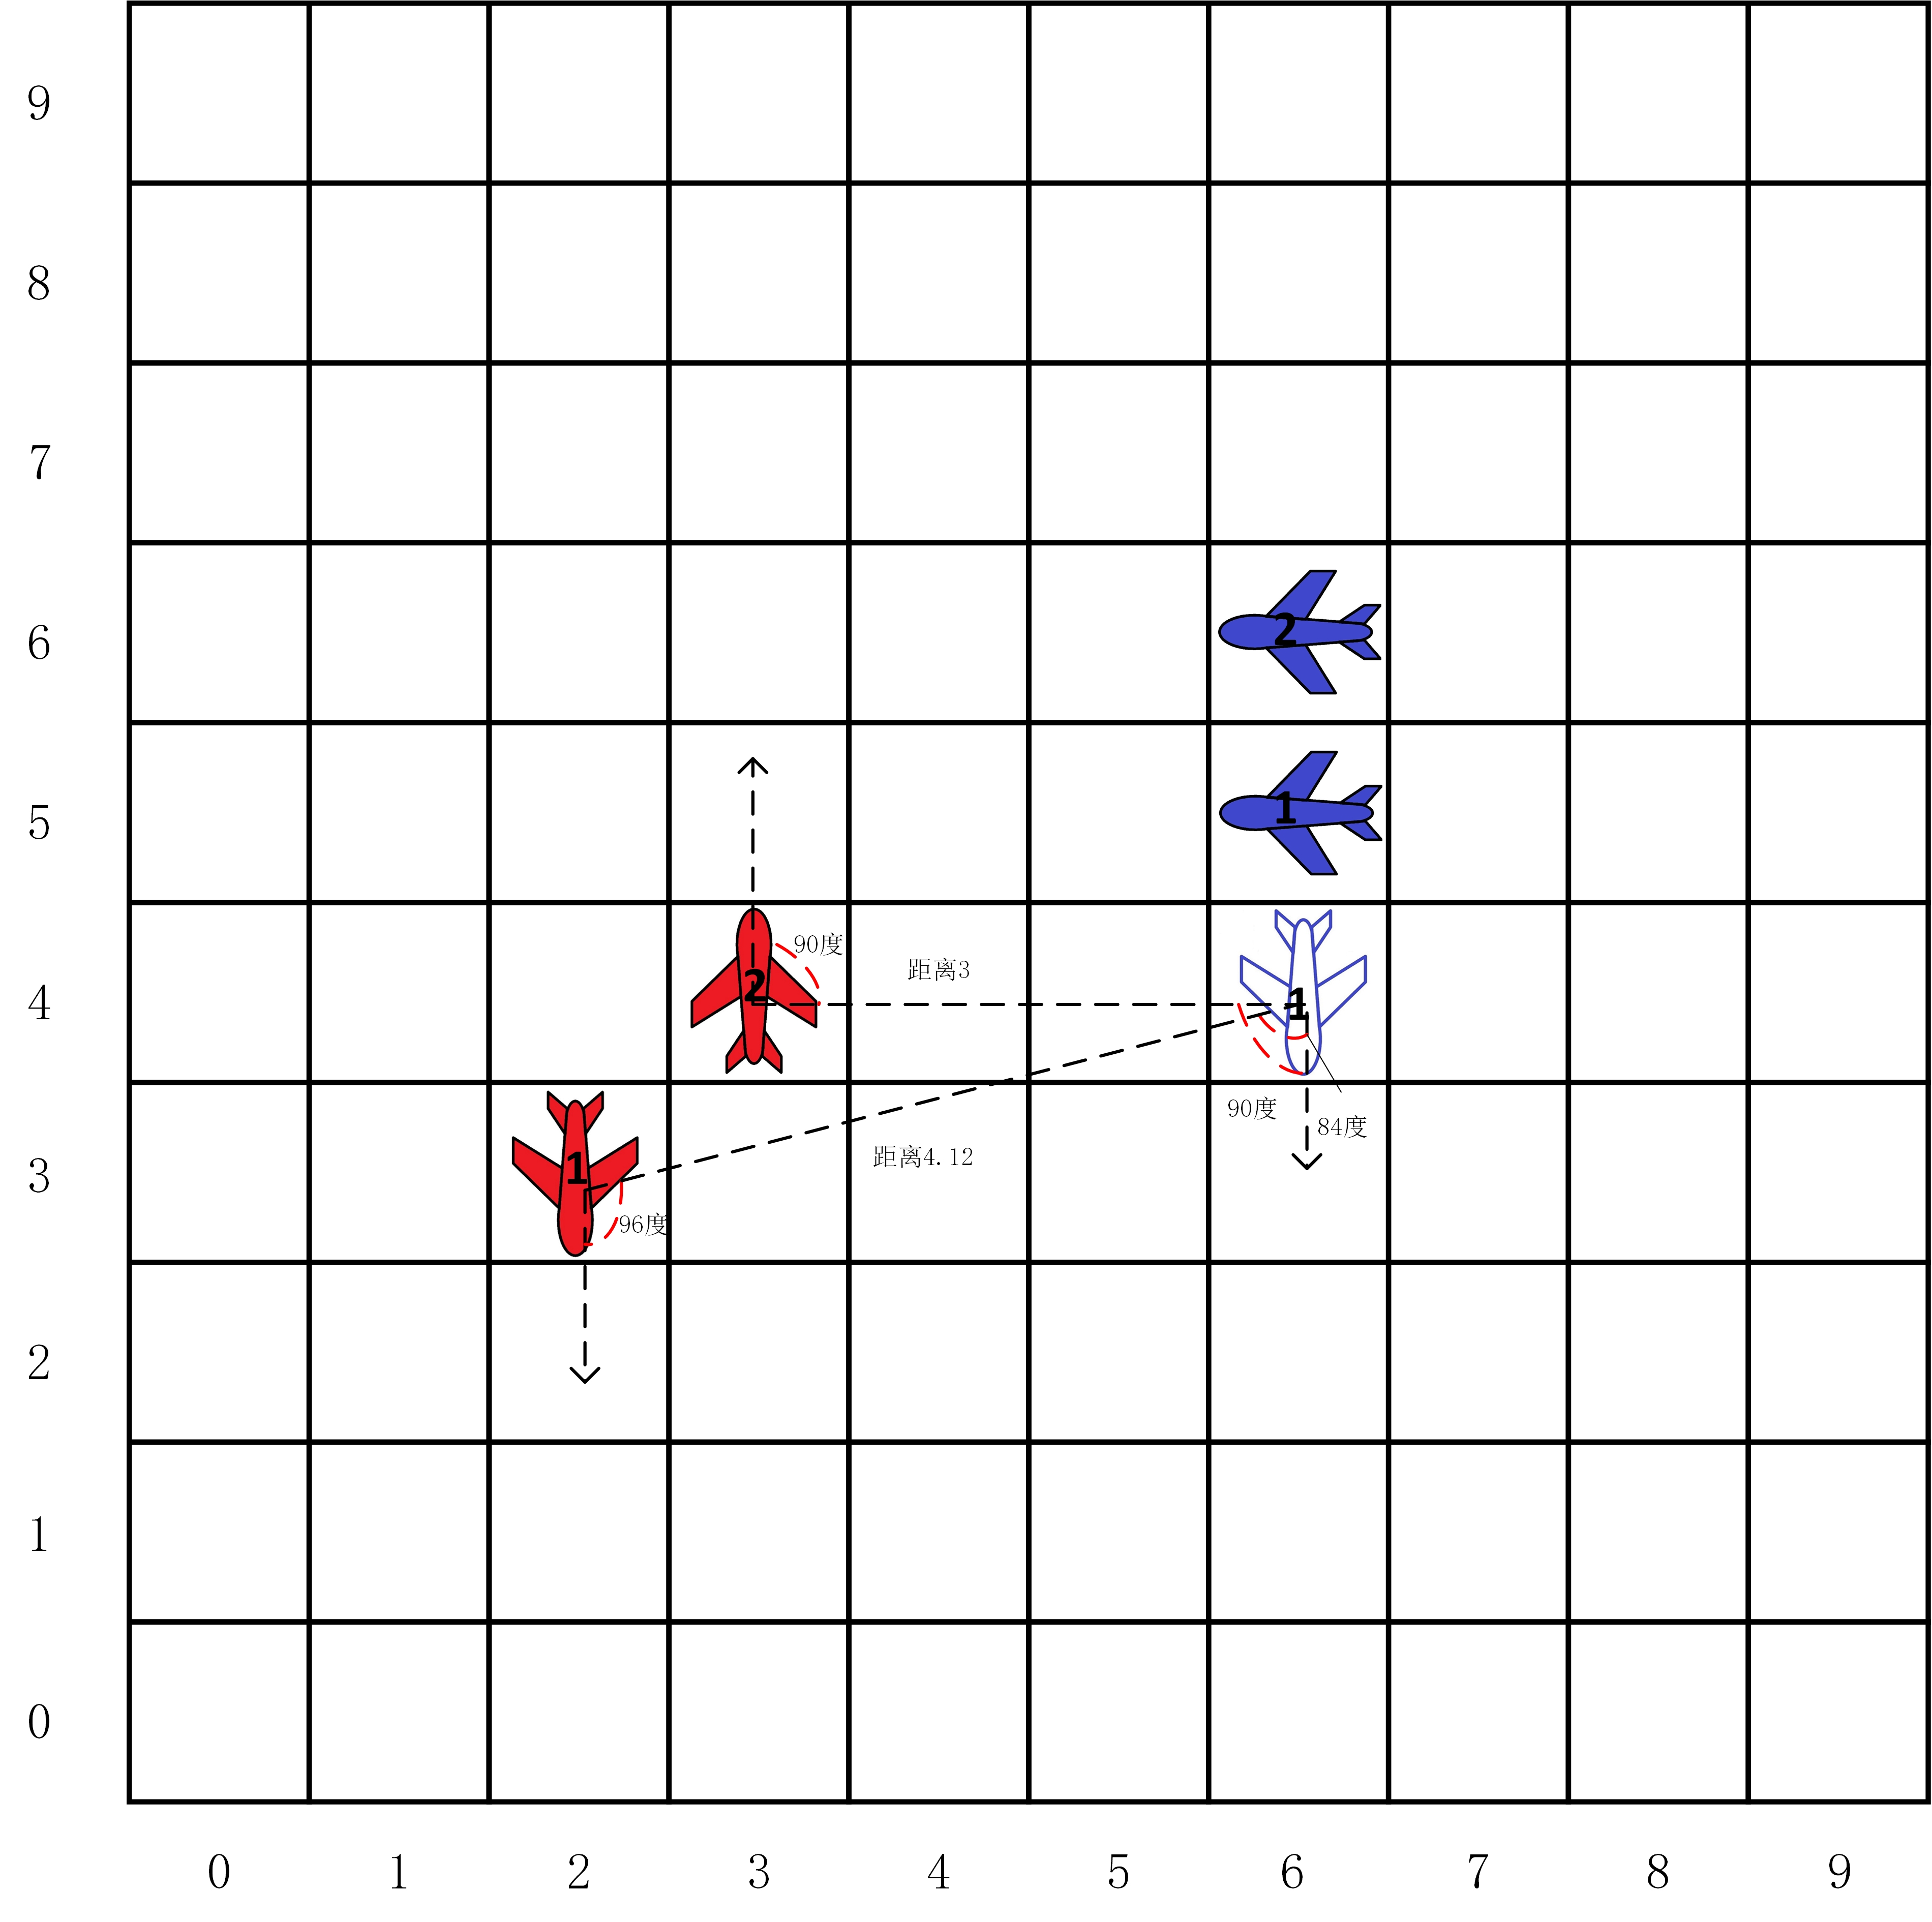
\includegraphics[width=0.45\hsize,height=0.45\hsize]{example/feijiduoduiduo7.jpg}}
	\hspace{0.5em}
	\subcaptionbox{向右状态\label{fig2:duoduiduo:b}}
	{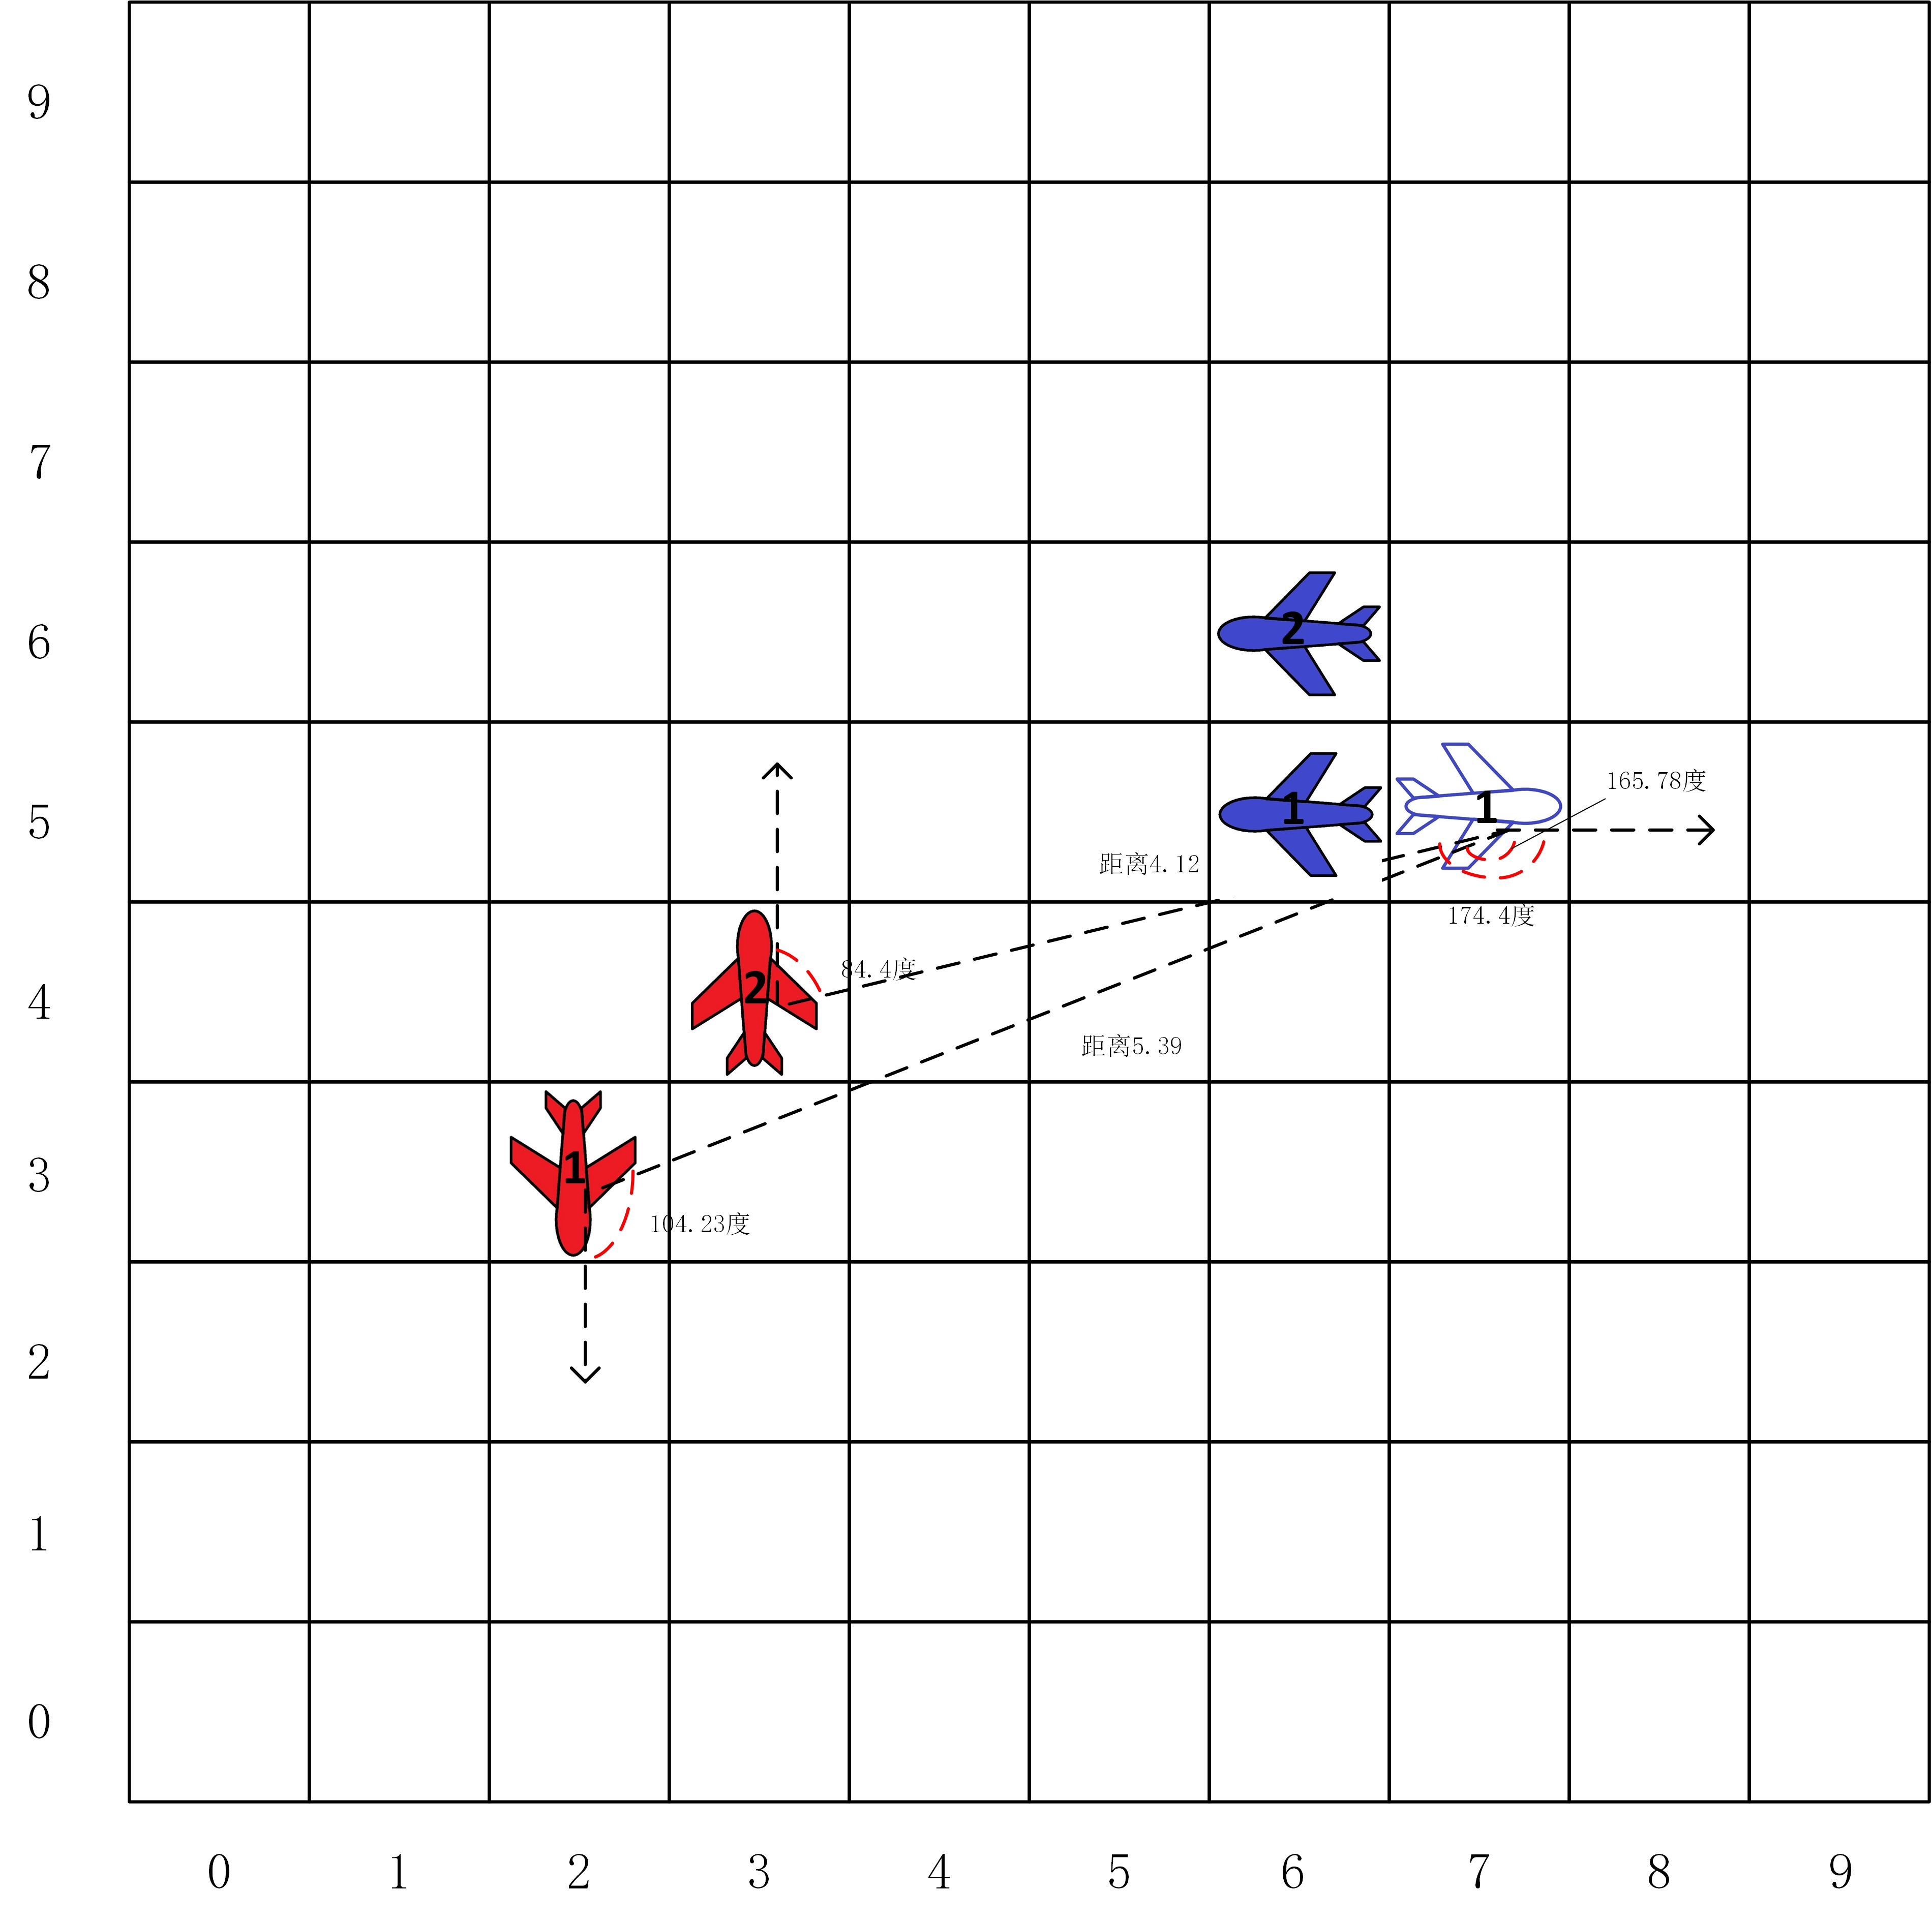
\includegraphics[width=0.45\hsize,height=0.45\hsize]{example/feijiduoduiduo8.jpg}}
	\bicaption[二对二对弈状态分析(1)]
	{二对二对弈状态分析(1)}
	{Game state analysis of four agents(1).}
	\label{fig2:duoduiduo}
\end{figure}
\begin{figure}[hpbt]
	\centering
	\subcaptionbox{向左状态\label{fig3:duoduiduo:a}}
	{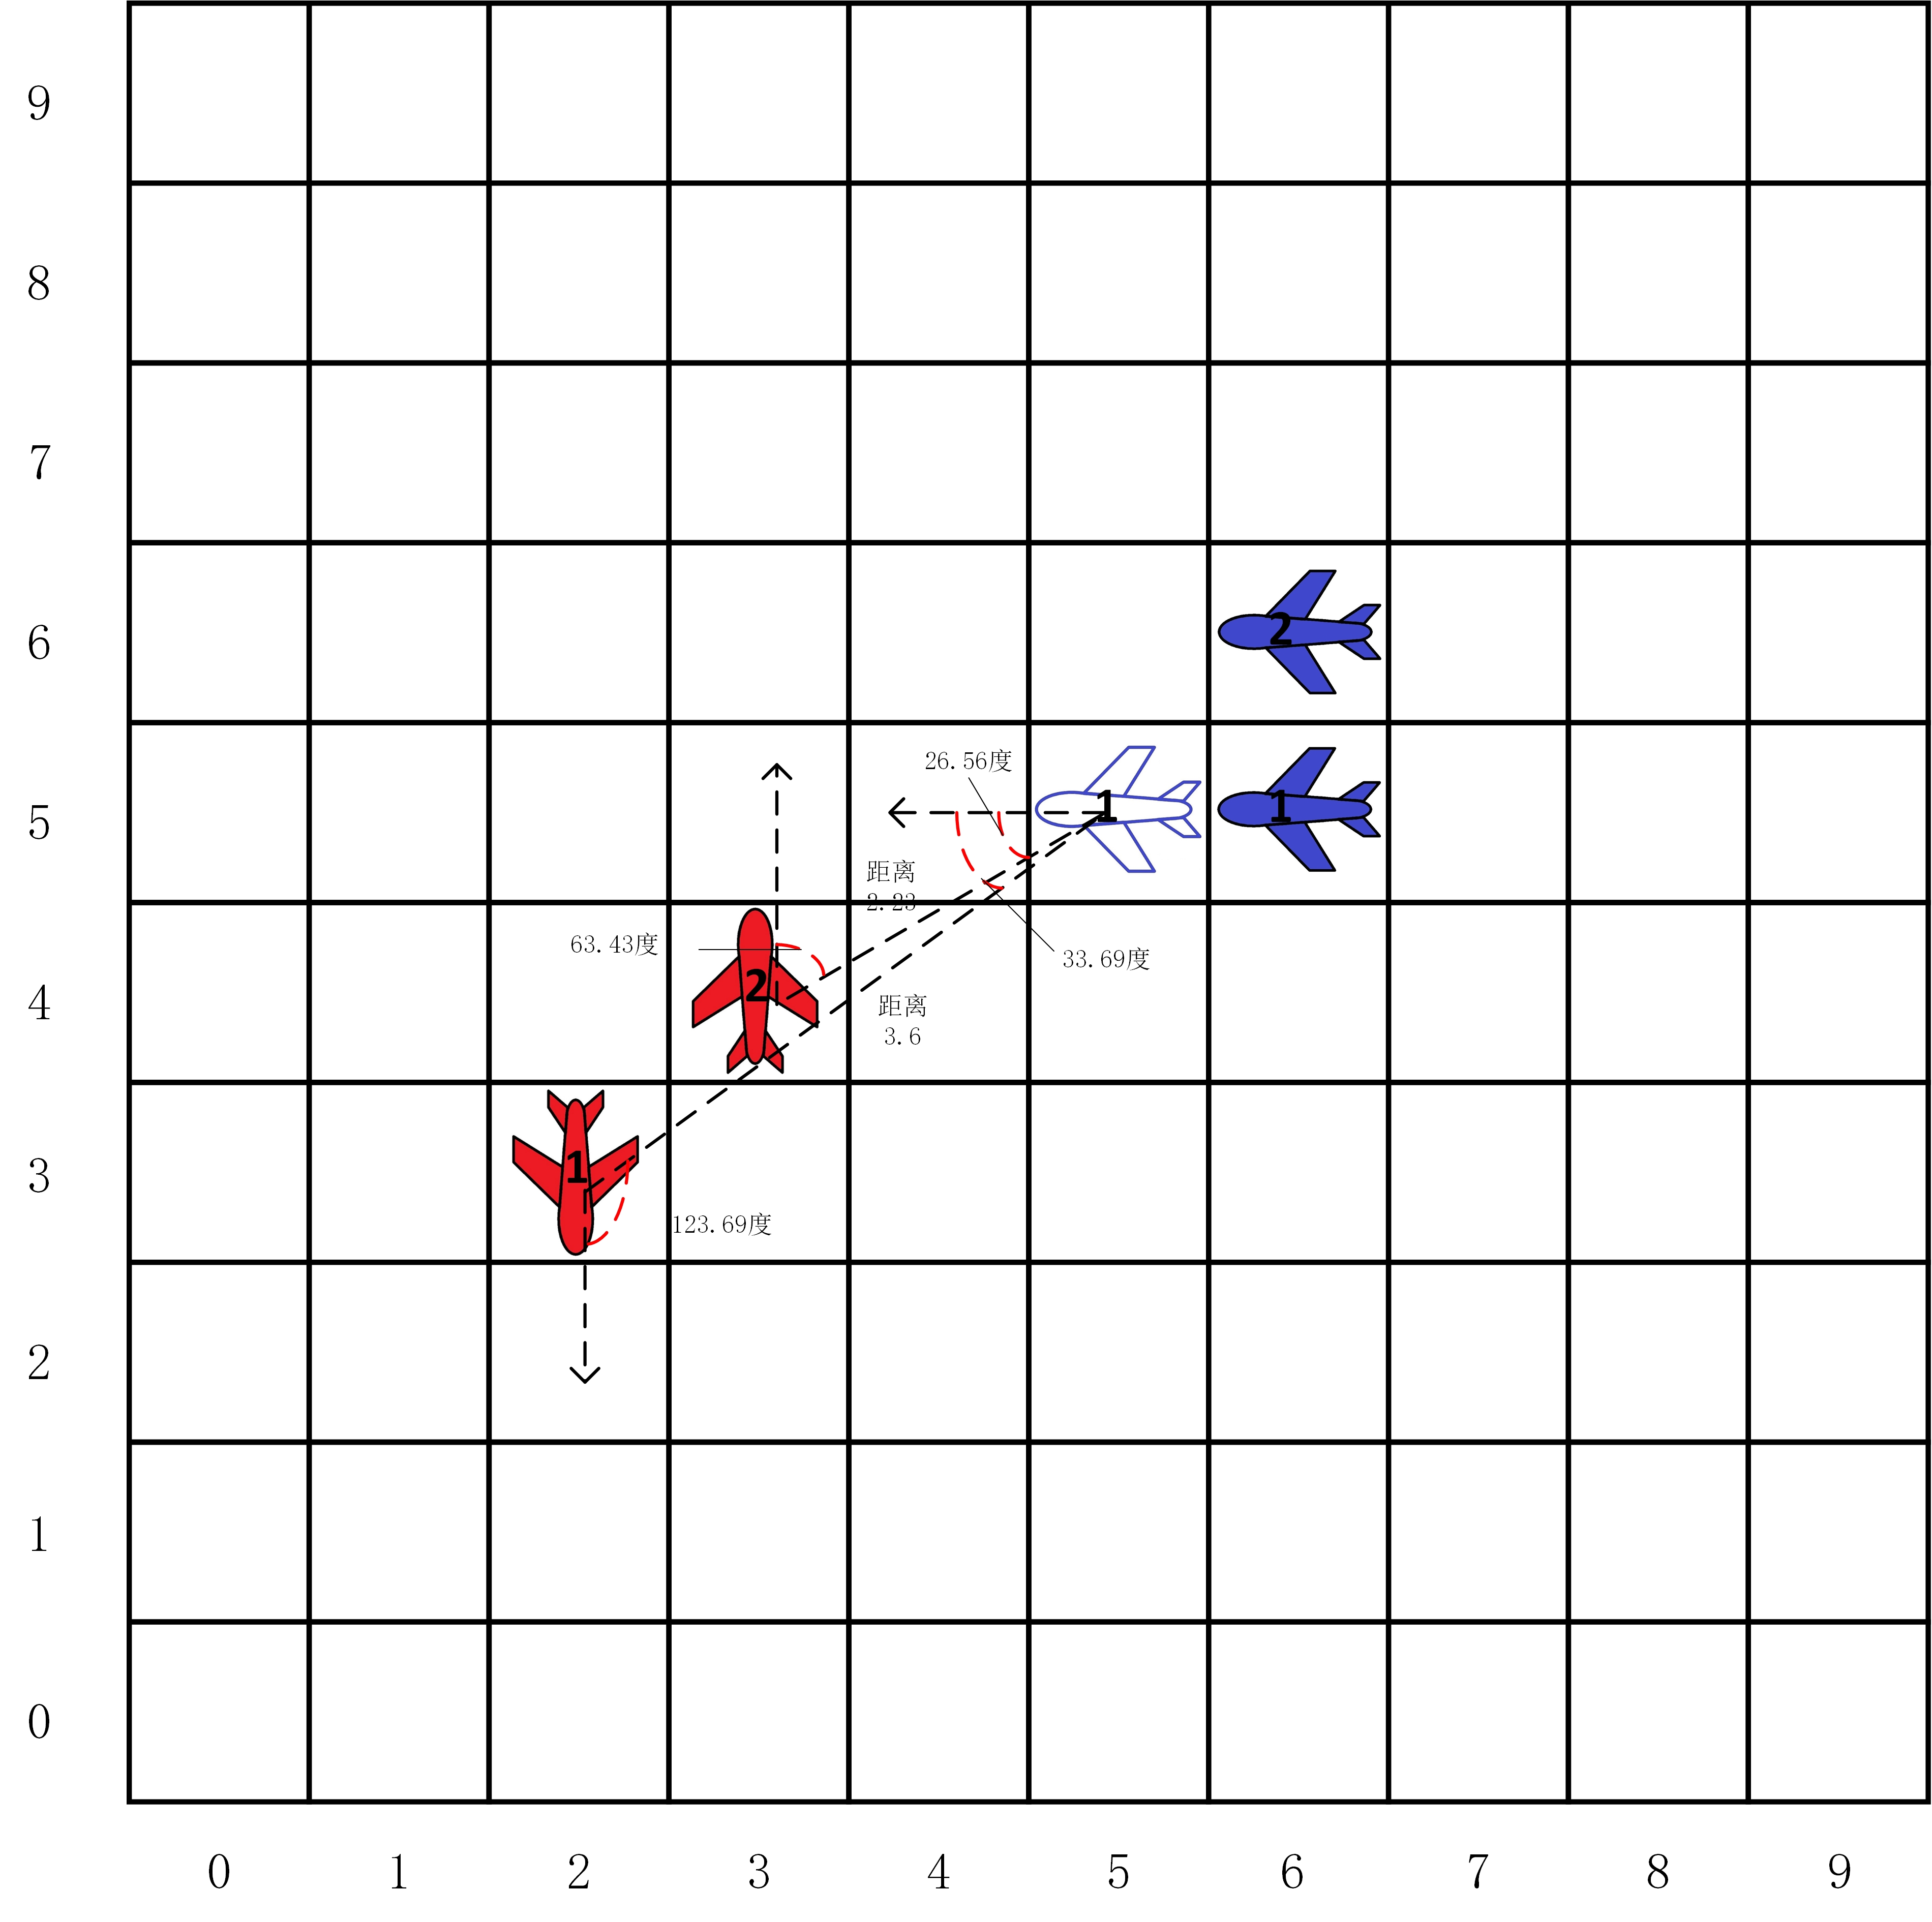
\includegraphics[width=0.45\hsize,height=0.45\hsize]{example/feijiduoduiduo9.jpg}}
	\hspace{0.5em}
	\subcaptionbox{最终结果\label{fig3:duoduiduo:b}}
	{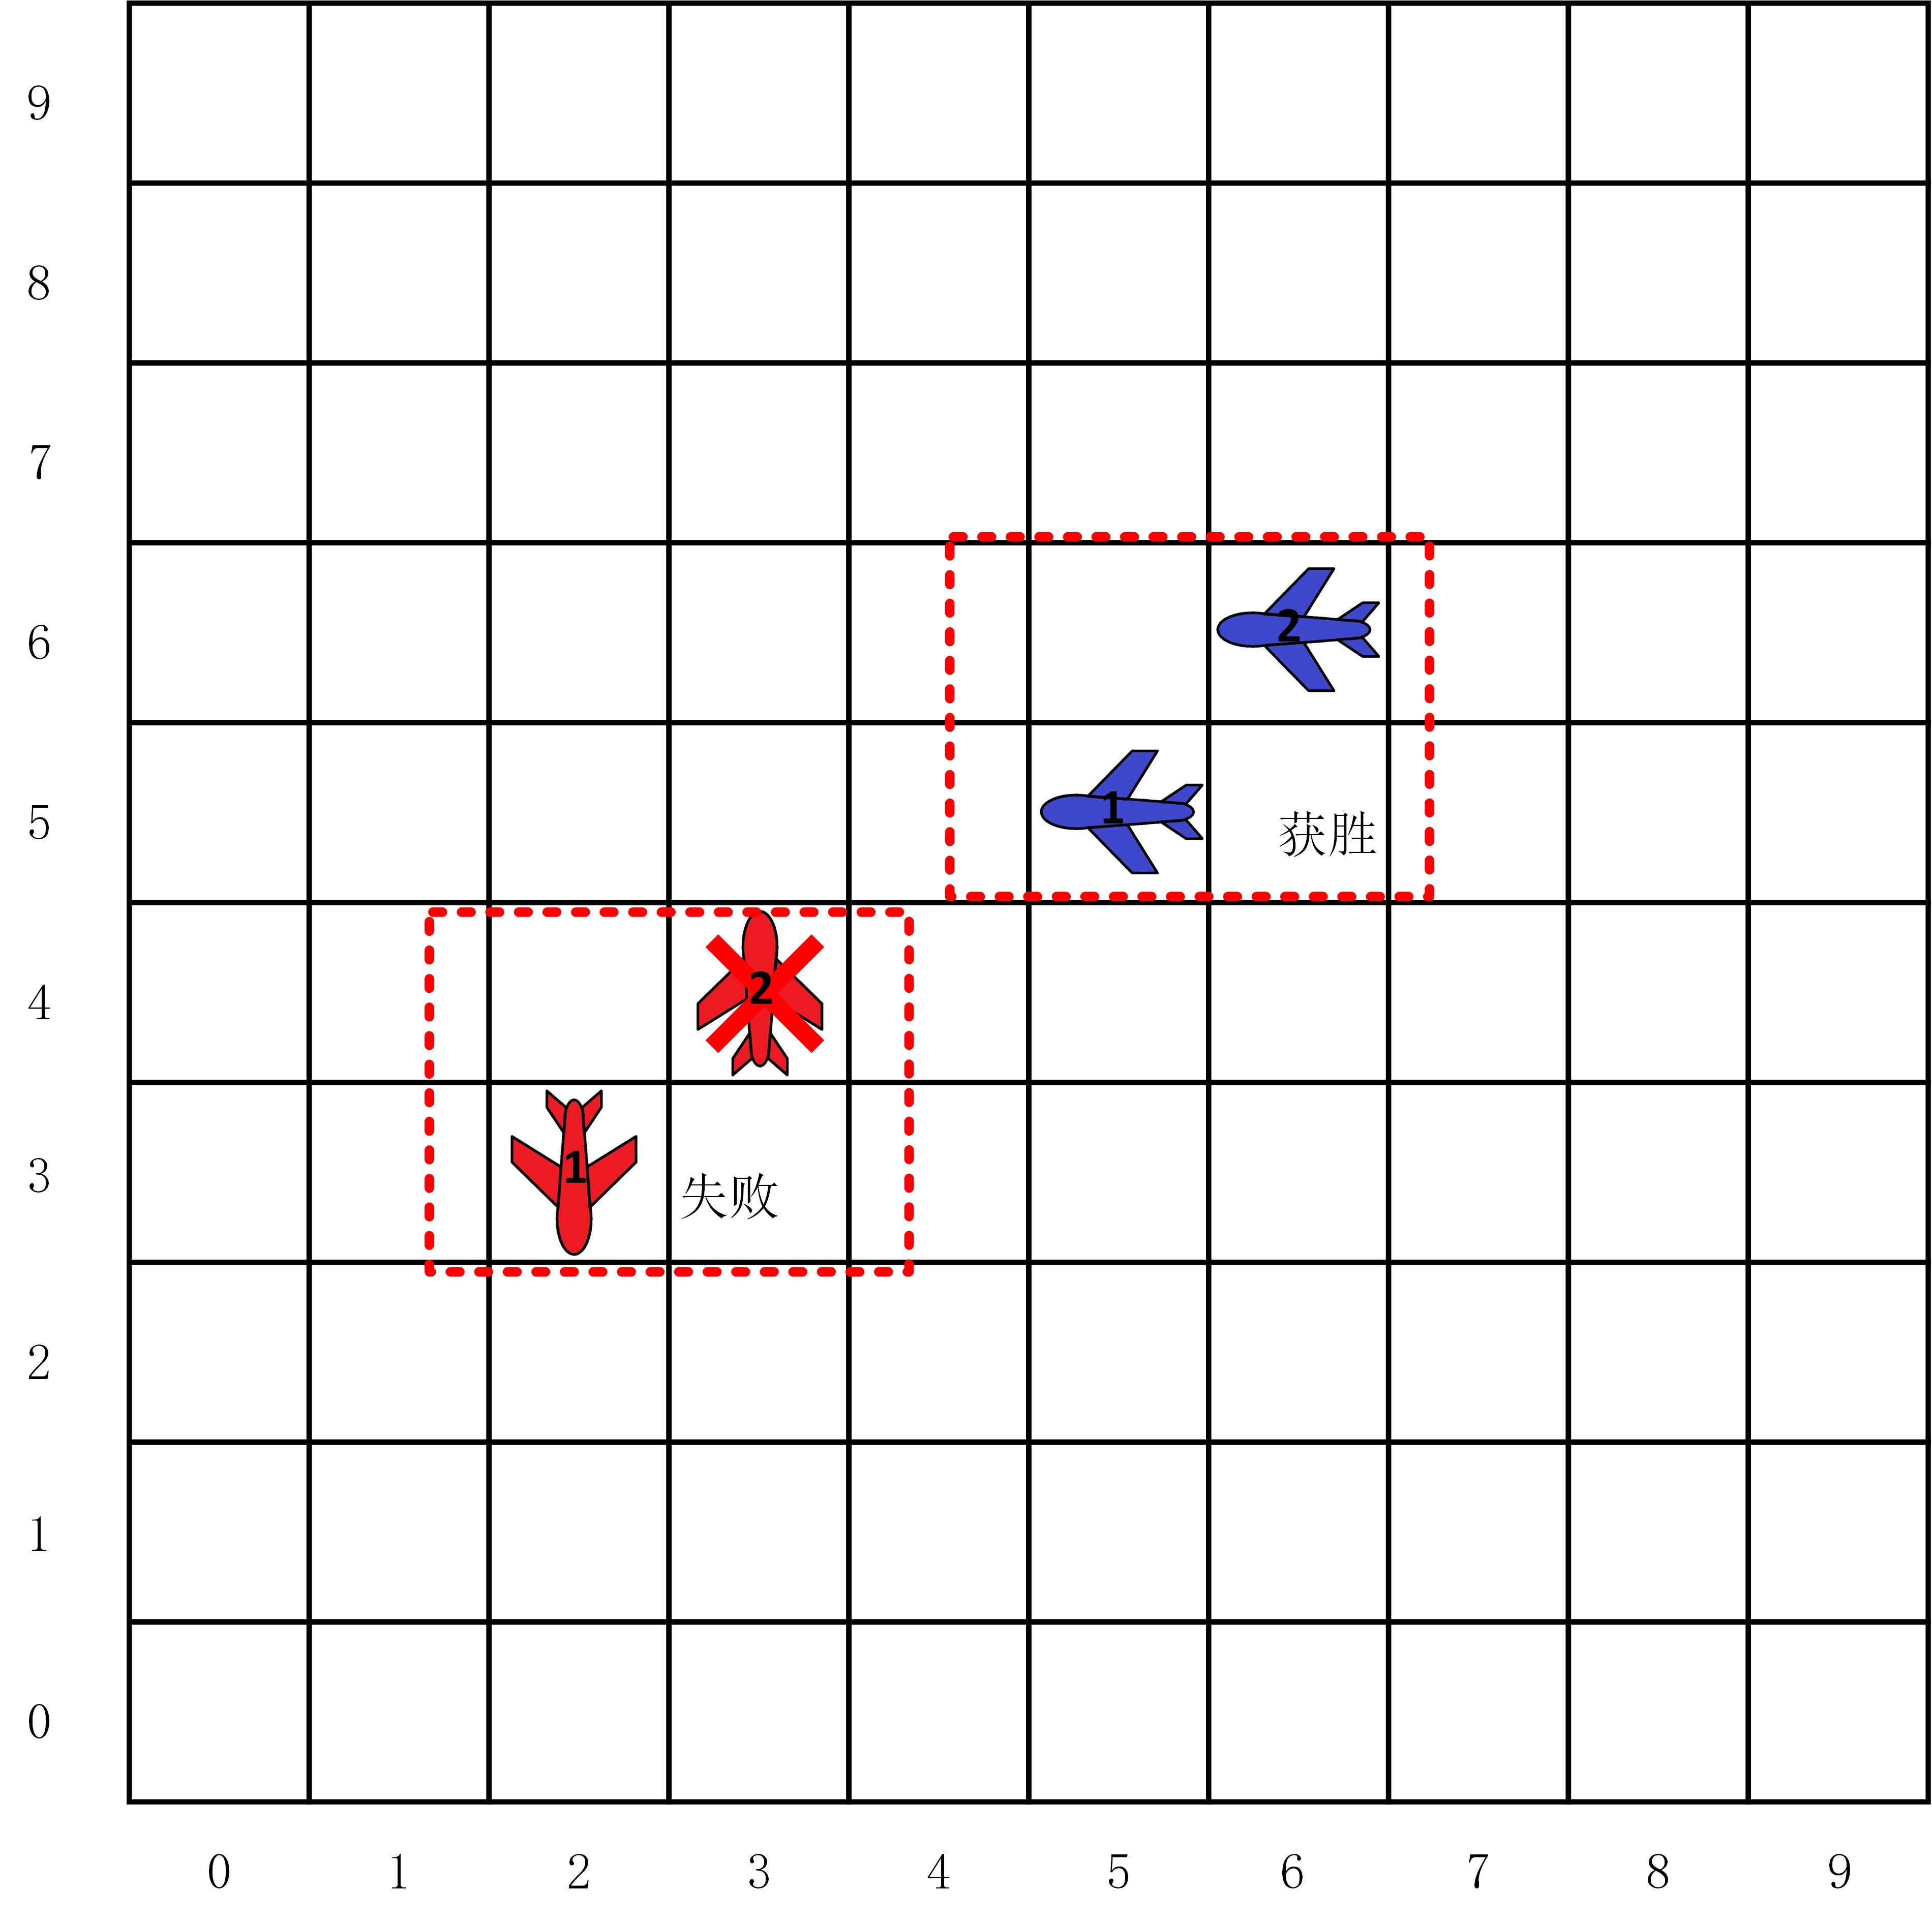
\includegraphics[width=0.45\hsize,height=0.45\hsize]{example/feijiduoduiduo10.jpg}}
	\bicaption[二对二对弈状态分析(2)]
	{二对二对弈状态分析(2)}
	{Game state analysis of four agents(2).}
	\label{fig3:duoduiduo}
\end{figure}


同时为了验证从零开始通过模型自我博弈得到数据的有效性,利用加入先验规则的模型和从零开始学习的模型进行对比,两个模型训练的参数设置相同,让其分别在模型迭代训练的前中后期进行50轮对弈。得到的对弈的结果如图\ref{fig:win}。

\begin{figure}[!hbtp]
	\centering
	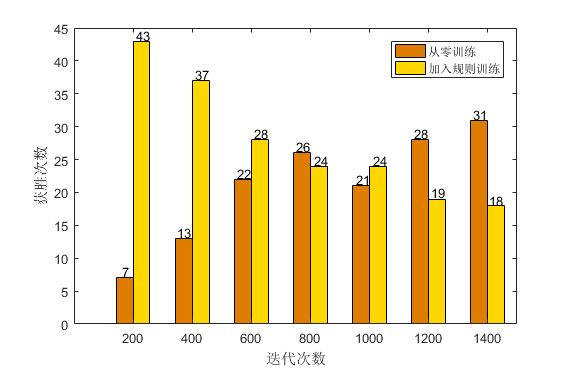
\includegraphics[width=10cm]{example/win.jpg}
	\bicaption[对弈统计结果]
	{对弈统计结果}
	{Game statistics results}
	\label{fig:win}
\end{figure}

可以看出在模型训练的初期,利用人类先验规则训练的模型由于收敛比较快,策略学习速度较快,具有很大的优势,在迭代到600到1200轮时,两个模型的胜负次数基本持平,而在训练后期无先验规则的模型具有更好的表现能力。
\subsubsection{合作关系分析}
在奖励分配上,图\ref{fig:duoduiduo3-6}和图\ref{fig:duoduiduo9-10}中红色数字为每次动作时奖励的分配,越接近对战过程的结局,预期奖励越大,符合实际情况即只有接近胜负才会得到明确反馈信号。同时分析蓝1蓝2的关系,在状态如图\ref{fig:duoduiduo3-6:d}时,蓝1获得的奖励最大为0.0722,当到达状态如图\ref{fig:duoduiduo9-10:b}蓝2执行最大奖励动作即向左时,蓝1获得最大奖励如图\ref{fig:duoduiduo9-10:d}为0.1124,可见,当蓝2靠近地方时,蓝1蓝2奖励同时增大。此时蓝1其他动作的奖励都为负值,向左获得奖励明显高于其他动作,符合上面分析的状态规律,即只有向左团队才会获得胜利。同样随着蓝1向最大奖励方向移动,蓝2也随着增大可能获得的奖励。最终蓝2奖励为0.1083,无论击灭地方飞机的是哪个智能体,团队成员所有飞机奖励都会相应增大,可见队内智能体已经具备一定的协作能力。

本节分析了二对二实验过程,对比了加入规则和不加规则的信息熵和损失函数的下降曲线,并分析了产生差异的原因,从结果上可以看到最后红一被击落,AI获胜,训练出来的模型具有一定的决策能力。在训练时需要合理平衡探索和利用的关系,在模型进行人机对抗时,采用贪婪策略选取概率最大的动作。实验分别从队间和队内进行了竞争合作关系的分析,可见模型具备自动分配奖励,进行决策的能力。同时利用从零开始学习模型的方案要比加入先验规则表现好,在模型前期可能会出现波动,但是在后期模型性能增长要比加入规则模型快。这也和由AlphaGo进化到AlphaZero得到的结果一致:在很多情况下利用人类专家数据学习的模型并不一定是最优的,让模型从白板开始训练,通过自我对弈进行能获得比人类认知更好的策略。

\section{本章小结}
本章主要针对飞机对战的问题进行了建模和分析。首先介绍了多智能体强化学习常用的算法,接着在第二部分介绍了一对一飞机对抗的强化学习算法实验,首先介绍了作战的背景,建模过程,包括状态空间的建立,动作的选择以及强化学习算法和搜索树的建立,对一对一作战的结果进行了展示和在不同状态下采取不同策略的态势分析。在第三部分由一对一对抗实验拓展到了二对二的实验,对于既有竞争又有合作的情况,首先介绍了应用的强化学习算法,接着进行了二对二实验的场景描述以及模型建立,设计网络结构和特征输入方式,然后对二对二的实验进行了结果展示,首先对比了有无人类规则情况下的训练曲线图,统计了两个模型之间博弈的结果。在详细展示了人机对弈过程后,分析了队间博弈关系和对内合作关系。可见利用深度强化学习做博弈模型的自主决策具有可行性,利用自博弈方式从零产生数据能学到更合理策略,同时实现了二对二智能体基于合作关系和竞争关系奖励的自动分配。

